% Options for packages loaded elsewhere
\PassOptionsToPackage{unicode}{hyperref}
\PassOptionsToPackage{hyphens}{url}
%
\documentclass[
]{scrbook}
\usepackage{amsmath,amssymb}
\usepackage{iftex}
\ifPDFTeX
  \usepackage[T1]{fontenc}
  \usepackage[utf8]{inputenc}
  \usepackage{textcomp} % provide euro and other symbols
\else % if luatex or xetex
  \usepackage{unicode-math} % this also loads fontspec
  \defaultfontfeatures{Scale=MatchLowercase}
  \defaultfontfeatures[\rmfamily]{Ligatures=TeX,Scale=1}
\fi
\usepackage{lmodern}
\ifPDFTeX\else
  % xetex/luatex font selection
\fi
% Use upquote if available, for straight quotes in verbatim environments
\IfFileExists{upquote.sty}{\usepackage{upquote}}{}
\IfFileExists{microtype.sty}{% use microtype if available
  \usepackage[]{microtype}
  \UseMicrotypeSet[protrusion]{basicmath} % disable protrusion for tt fonts
}{}
\makeatletter
\@ifundefined{KOMAClassName}{% if non-KOMA class
  \IfFileExists{parskip.sty}{%
    \usepackage{parskip}
  }{% else
    \setlength{\parindent}{0pt}
    \setlength{\parskip}{6pt plus 2pt minus 1pt}}
}{% if KOMA class
  \KOMAoptions{parskip=half}}
\makeatother
\usepackage{xcolor}
\usepackage{longtable,booktabs,array}
\usepackage{calc} % for calculating minipage widths
% Correct order of tables after \paragraph or \subparagraph
\usepackage{etoolbox}
\makeatletter
\patchcmd\longtable{\par}{\if@noskipsec\mbox{}\fi\par}{}{}
\makeatother
% Allow footnotes in longtable head/foot
\IfFileExists{footnotehyper.sty}{\usepackage{footnotehyper}}{\usepackage{footnote}}
\makesavenoteenv{longtable}
\usepackage{graphicx}
\makeatletter
\def\maxwidth{\ifdim\Gin@nat@width>\linewidth\linewidth\else\Gin@nat@width\fi}
\def\maxheight{\ifdim\Gin@nat@height>\textheight\textheight\else\Gin@nat@height\fi}
\makeatother
% Scale images if necessary, so that they will not overflow the page
% margins by default, and it is still possible to overwrite the defaults
% using explicit options in \includegraphics[width, height, ...]{}
\setkeys{Gin}{width=\maxwidth,height=\maxheight,keepaspectratio}
% Set default figure placement to htbp
\makeatletter
\def\fps@figure{htbp}
\makeatother
\setlength{\emergencystretch}{3em} % prevent overfull lines
\providecommand{\tightlist}{%
  \setlength{\itemsep}{0pt}\setlength{\parskip}{0pt}}
\setcounter{secnumdepth}{5}
% definitions for citeproc citations
\NewDocumentCommand\citeproctext{}{}
\NewDocumentCommand\citeproc{mm}{%
  \begingroup\def\citeproctext{#2}\cite{#1}\endgroup}
\makeatletter
 % allow citations to break across lines
 \let\@cite@ofmt\@firstofone
 % avoid brackets around text for \cite:
 \def\@biblabel#1{}
 \def\@cite#1#2{{#1\if@tempswa , #2\fi}}
\makeatother
\newlength{\cslhangindent}
\setlength{\cslhangindent}{1.5em}
\newlength{\csllabelwidth}
\setlength{\csllabelwidth}{3em}
\newenvironment{CSLReferences}[2] % #1 hanging-indent, #2 entry-spacing
 {\begin{list}{}{%
  \setlength{\itemindent}{0pt}
  \setlength{\leftmargin}{0pt}
  \setlength{\parsep}{0pt}
  % turn on hanging indent if param 1 is 1
  \ifodd #1
   \setlength{\leftmargin}{\cslhangindent}
   \setlength{\itemindent}{-1\cslhangindent}
  \fi
  % set entry spacing
  \setlength{\itemsep}{#2\baselineskip}}}
 {\end{list}}
\usepackage{calc}
\newcommand{\CSLBlock}[1]{\hfill\break\parbox[t]{\linewidth}{\strut\ignorespaces#1\strut}}
\newcommand{\CSLLeftMargin}[1]{\parbox[t]{\csllabelwidth}{\strut#1\strut}}
\newcommand{\CSLRightInline}[1]{\parbox[t]{\linewidth - \csllabelwidth}{\strut#1\strut}}
\newcommand{\CSLIndent}[1]{\hspace{\cslhangindent}#1}
% fonts
% libertine font: https://www.tug.org/FontCatalogue/linuxlibertine/
\usepackage[oldstyle]{libertine}
\usepackage{libertinust1math}
% \usepackage[T1]{fontenc}
\usepackage[extralight]{inter} 

\usepackage[left=3cm, right=2.5cm, top=2.5cm, bottom=4cm]{geometry} % page margings

\usepackage{tabto} % for aligning text at a certain position, used for title page

\usepackage{booktabs}	
\usepackage{multirow} % use multirow for tables
\usepackage{float} % needed by [H] (i.e., HERE)
\usepackage{caption}
\captionsetup{labelformat=empty}

\usepackage[ngerman, english]{babel}		% main language is the last in the list, more infor is here: https://en.wikibooks.org/wiki/LaTeX/Internationalization#Babel

\usepackage[onehalfspacing]{setspace}	% clean 1.5 leading / spacing
\RedeclareSectionCommand[beforeskip=1em,afterskip=2em]{chapter} % define space before and after heading

\usepackage{pdfpages} % to include pdfs

\usepackage{hanging} % for hanging indents on title page

% \hypersetup{
% 	unicode=true,          % non-Latin characters in Acrobat’s bookmarks
% 	pdftitle={Rethinking Variation in Social Cognition: Gaze Following across Individuals, Ages, and Communities},    % title
% 	pdfauthor={Julia Christin Prein},     % author
% 	pdfsubject={Dissertation},   % subject of the document
% 	pdfcreator={Julia Christin Prein},   % creator of the document
% 	pdfproducer={Julia Christin Prein}, % producer of the document
% 	pdfkeywords={Social Cognition, Gaze Following, Child Development, Psychometrics, Individual Differences, Cross-cultural Research}, % list of keywords
% 	pdfnewwindow=true,      % links in new PDF window
% 	colorlinks=true,       % false: boxed links; true: colored links
% 	pdfborder={0 0 0},		% color of the border around links
% 	linkbordercolor={0 0 0},
% 	citebordercolor={0 0 0},
% 	urlbordercolor={0 0 0},
% 	linktoc=page,				% defines which part of an entry in the table of contents is made into a link (none,section,page,all)
% 	linkcolor=MidnightBlue,          % color of internal links (change box color with linkbordercolor)
% 	citecolor=MidnightBlue,        % color of links to bibliography
% 	filecolor=MidnightBlue,      % color of file links
% 	urlcolor=MidnightBlue           % color of external links
% }
\ifLuaTeX
  \usepackage{selnolig}  % disable illegal ligatures
\fi
\usepackage{bookmark}
\IfFileExists{xurl.sty}{\usepackage{xurl}}{} % add URL line breaks if available
\urlstyle{same}
\hypersetup{
  hidelinks,
  pdfcreator={LaTeX via pandoc}}

\author{}
\date{\vspace{-2.5em}}

\begin{document}

\frontmatter

\begin{titlepage}                   
    \begin{center}
        
\includegraphics[height=3.2cm]{logo.pdf}\\[40mm]
        
        \huge {\linespread{1.5} Rethinking Variation in Social Cognition: \\ Gaze Following Across Individuals, Ages, and Communities}\\[30mm]
        
                
        \normalsize 
        Faculty of Sustainability \\ 
        at Leuphana University Lüneburg\\
        Submitted as a requirement for the award of the title of\\ [10mm]
        
        Doctor of Psychology\\
        -- Dr. rer. nat. --\\[10mm]
        
        Approved dissertation by\\
        Julia Christin Prein\\[10mm]
        
        born February 26, 1995 in Berlin-Kreuzberg, Germany
        
    \vspace*{\fill} 
    \end{center}
    
    \newpage
    \thispagestyle{empty}
    \begin{flushleft}
      \begin{normalsize}
      \vspace*{5mm}
      
            Submitted on: \tabto*{45mm} October 1, 2024 \\
            
            Oral thesis defense on: \tabto*{45mm} February 26, 2025 \\
            
            Year of publication: \tabto*{45mm} 2025 \\[10mm]
            
            Supervisors and examiners (alphabetically ordered): \\[5mm]
            \tabto*{5mm} Prof.\,Dr.\, Manuel Bohn, \textit{Leuphana University Lüneburg}\\
            \tabto*{5mm} Prof.\,Dr.\, Daniel Haun, \textit{Leipzig University \& Max Planck Institute for Evolutionary Anthropology}\\
                \tabto*{5mm} Prof.\,Dr.\, Sebastian Wallot, \textit{Leuphana University Lüneburg}\\[10mm]
                
                The individual publications in the cumulative thesis are included in Appendix A of this framework paper and are or will be published as follows: \\[5mm]
                
                \begin{hangparas}{5mm}{1}

Prein, J. C., Kalinke, S., Haun, D. B. M.\*, \& Bohn, M.\* (2024). TANGO: A reliable, open-source, browser-based task to assess individual differences in gaze understanding in 3 to 5-year-old children and adults. \textit{Behavior Research Methods, 56}(3), 2469–2485. \mbox{\url{https://doi.org/10.3758/s13428-023-02159-5}} \\[5mm]

Prein, J. C., Maurits, L., Werwach, A., Haun, D. B. M.,\* \& Bohn, M.\* (2024). Variation in gaze following across the life span: A process-level perspective. \textit{Developmental Science}, Article e13546. \mbox{\url{https://doi.org/10.1111/desc.13546}} \\[5mm]

Bohn, M.\*, Prein, J. C.\*, Ayikoru, A., Bednarski, F. M., Dzabatou, A., Frank, M. C., Henderson, A. M. E., Isabella, J., Kalbitz, J., Kanngiesser, P., Keşşafoğlu, D., Koymen, B., Manrique-Hernandez, M., Magazi, S., Mújica-Manrique, L., Ohlendorf, J., Olaoba, D., Pieters, W., Pope-Caldwell, S., … Haun, D. (2024). \textit{A universal of human social cognition: Children from 17 communities process gaze in similar ways} [Manuscript submitted for publication]. PsyArXiv. \mbox{\url{https://doi.org/10.31234/osf.io/z3ahv}} \\[5mm]

Prein, J. C., Bednarski, F. M., Dzabatou, A., Frank, M. C., Henderson, A. M. E., Kalbitz, J., Kanngiesser, P., Keşşafoğlu, D., Koymen, B., Manrique-Hernandez, M., Magazi, S., Mújica-Manrique, L., Ohlendorf, J., Olaoba, D., Pieters, W., Pope-Caldwell, S., Sen, U., Slocombe, K., Sparks, R. Z., … Bohn, M. (2024). \textit{Measuring variation in gaze following across communities, ages, and individuals – a showcase of the TANGO–CC} [Manuscript submitted for publication]. PsyArxiv. \mbox{\url{https://doi.org/10.31234/osf.io/fcq2g}}

                \end{hangparas}
        \end{normalsize}
    \end{flushleft}
    
\end{titlepage}

\chapter{Abstract}\label{abstract}

Social cognition enables children to engage effectively with peers, teachers, and family, making them active members of society. Throughout childhood, individuals learn to collaborate efficiently, predict future actions, and reason about the desires, beliefs, and percepts of themselves and others. The bedrock of many social-cognitive abilities is gaze following: Identifying another's attentional focus is valuable for extracting information from the environment and determining the internal states of other agents. The emergence of gaze following has been thoroughly studied on a group level in children from the Global North. Yet, we know little about individual-level and cross-cultural variation. This is problematic because many developmental theories emphasize the role of social interaction in the development of social cognition\thinspace --\thinspace and the frequency and characteristics of social interactions vary substantially across individuals and cultures. This dissertation aims to highlight the prevalence and importance of variation in social cognition based on the example of gaze following. In four studies, we have designed a new gaze following task and applied it to capture individual- and community-level variation in this core social-cognitive ability.

Study I focused on the development and psychometric assessment of the new task, the TANGO (Task for Assessing iNdividual Differences in Gaze understanding-Open). An animated interactive picture book asked participants to locate a balloon with the help of a gaze cue. A spatial layout allowed for a discrete and continuous measure of participants' imprecision in locating the attentional focus. We implemented a new interactive web application that works across devices and enables supervised and unsupervised in-person and remote testing. We found substantial individual differences in a child (\emph{N}\thinspace=\thinspace 387 from Leipzig, Germany) and an adult (\emph{N}\thinspace =\thinspace 236, international remote) sample. Good psychometric properties, in the form of high internal consistency and test-retest reliability, indicated highly systematic variation. Relationships with family-level variables and children's language abilities underline the validity of the task. Together, the results show how the TANGO is a reliable and valid tool to assess individual differences in gaze following.

Study II applied the TANGO to three research questions focusing on individual differences in gaze following. First, we examined gaze following across the lifespan (\emph{N}\thinspace =\thinspace 478 3- to 19-year-olds from Leipzig, Germany, and \emph{N}\thinspace =\thinspace 240 20- to 80-year-old international, remotely tested adults). During preschool years, children became increasingly precise in gaze following and reached adult-like performance with around ten years of age. Young adults reached the highest precision levels, which slightly declined toward old age. Across all age groups, participants showed individual differences. Second, we conceptualized individual differences in gaze following in a computational cognitive model (\emph{N}\thinspace =\thinspace 60 3- to 5-year-olds and \emph{N}\thinspace =\thinspace 50 adults). Participants were modeled to observe the agent's pupil location within the eye and estimate the resulting pupil angles and gaze vectors. This inferential estimation process was assumed to be noisy. Individual differences and the development of gaze following were described as varying levels in the precision to estimate pupil angles. A model comparison with two alternative models and a signature pattern in the data yielded strong evidence for the proposed gaze model. Third, we experimentally tested the model's assumption describing gaze following as a form of social vector estimation (\emph{N}\thinspace =\thinspace 102 4- to 5-year-olds). Individuals' gaze-following abilities correlated with their precision in non-social vector estimation and visual perspective-taking. Other Theory of Mind tasks did not correlate. These findings suggest that gaze following relies on attention to social as well as spatial components.

Study III presented the largest cross-cultural study on children's gaze following abilities to this date (\emph{N}\thinspace =\thinspace 1377): We studied 2.5- to 11-year-olds from 17 different urban/rural communities in Argentina, China, the Democratic Republic of Congo, Germany, India, Mexico, Namibia, Nigeria, New Zealand, Sambia, Türkiye, the UK, Uganda, and the USA. Across communities, we found similar substantial developmental gains: With increasing age, children became more precise in locating the attentional focus of another agent. Absolute differences in imprecision levels could be partially explained by children's familiarity with the data collection device (tablet/touchscreen). In all communities, we found the same signature pattern in the data, and comparisons to alternative models provided strong evidence for the previously proposed gaze model. Despite existing individual- and community-level variation in observable behavior, this speaks for a universal mechanism in how children follow gaze.

Study IV describes the design process of the TANGO-CC, the cross-cultural gaze following task we used in Study III. We provided an open-source website and tutorial for researchers to adapt the TANGO-CC to their needs (e.g., selecting language and stimuli). Re-analyzing the data set of Study III, we found individual differences across communities and within-community variation outweighed between-community variation. Most importantly, we found satisfactory split-half reliability estimates for each community. These findings indicated the TANGO-CC's suitability for cross-cultural research.

Taken together, this dissertation takes an innovative, extensive, multifaceted perspective on gaze following and the cognitive processes behind it. It highlights how combining individual differences, cross-cultural research, and formal modeling will enable us to explore the development and structure of our core social-cognitive processes in greater detail.

\chapter{Zusammenfassung}\label{zusammenfassung}

Soziale Kognition ermöglicht es Kindern, erfolgreich mit Gleichaltrigen, Pädagog*innen und der Familie zu interagieren und eigenständige Mitglieder der Gesellschaft zu werden. Im Laufe der Kindheit lernen wir, effizient zu kooperieren, zukünftige Handlungen vorherzusagen und über die Wünsche, Überzeugungen und Wahrnehmungen von uns selbst und anderen nachzudenken. Die Grundlage vieler sozial-kognitiver Fähigkeiten ist die Blickverfolgung: Den Aufmerksamkeitsfokus eines Gegenübers zu identifizieren ist wegweisend, um Informationen aus der Umwelt und über die mentalen Zustände anderer zu gewinnen. Die Blickverfolgung ist auf Gruppenebene bei Kindern aus dem Globalen Norden gründlich untersucht. Jedoch wissen wir nur wenig über individuelle und kulturübergreifende Unterschiede. Dies ist problematisch, da viele Entwicklungstheorien die Rolle der sozialen Interaktion bei der Entwicklung sozialer Kognition betonen und die Häufigkeit und Merkmale sozialer Interaktionen zwischen Individuen und Kulturen erheblich variieren. Diese Dissertation soll die Bedeutsamkeit von Variation in der sozialen Kognition am Beispiel der Blickverfolgung aufzeigen. In vier Studien haben wir eine neue Aufgabe zur Blickverfolgung entwickelt, um Variation auf individueller und Gemeinschaftsebene messbar zu machen.

Studie I befasste sich mit der Entwicklung und psychometrischen Überprüfung der neuen Aufgabe, dem TANGO. Ein animiertes interaktives Bilderbuch forderte die Teilnehmenden auf, der Blickrichtung eines Anderen zu folgen, um einen Luftballon zu finden. Durch ein räumliches Layout konnten wir die Ungenauigkeit von Teilnehmenden in der Blickverfolgung diskret und kontinuierlich messen. Wir haben eine neue interaktive Web-Anwendung implementiert, die geräteübergreifend funktioniert und Datenerhebungen beaufsichtigt vor Ort, wie unbeaufsichtigt unterwegs ermöglicht. Wir fanden erhebliche individuelle Unterschiede in einer Kinder- (\emph{N}\thinspace=\thinspace 387 aus Leipzig, Deutschland) und einer Erwachsenenstichprobe (\emph{N}\thinspace =\thinspace 236 international verteilt). Die psychometrischen Eigenschaften, basierend auf interner Konsistenz und Test-Retest-Reliabilität, wiesen auf sehr systematische Variation hin. Zusammenhänge mit Variablen auf familiärer Ebene und sprachlichen Fähigkeiten unterstreichen die Validität der Aufgabe. Insgesamt ist der TANGO ein zuverlässiges und valides Instrument, um individuelle Unterschiede in der Blickverfolgung zu erfassen.

In Studie II haben wir den TANGO auf drei Forschungsfragen angewandt, die sich auf individuelle Unterschiede in der Blickverfolgung konzentrieren. Als Erstes untersuchten wir die Blickverfolgung über die Lebensspanne (\emph{N}\thinspace =\thinspace 478 3- bis 19-jährige Kinder aus Leipzig, Deutschland und \emph{N}\thinspace =\thinspace 240 20- bis 80-jährige internationale Erwachsene). Im Laufe des Vorschulalters wurden Kinder zunehmend präziser, den Blickrichtungen anderer zu folgen. Junge Erwachsene erreichten die höchste Genauigkeit, die mit zunehmendem Alter leicht abnahmen. Über alle Altersgruppen hinweg zeigten die Teilnehmenden individuelle Unterschiede. Zweitens konzeptualisierten wir individuelle Unterschiede in der Blickverfolgung in einem kognitiven Computermodell (\emph{N}\thinspace =\thinspace 60 3- bis 5-Jährige und \emph{N}\thinspace =\thinspace 50 Erwachsene). Das Modell beschreibt, dass die Teilnehmenden die Position der Pupille im Auge des Gegenübers beobachten und die daraus resultierenden Pupillenwinkel und Blickvektoren schätzen. Dieser inferentielle Schätzprozess kann fehlerhaft sein. Individuelle Unterschiede und die Altersentwicklung in der Blickverfolgung wurden modelliert durch unterschiedlich genaue Schätzungen der Pupillenwinkel. Durch einen Modellvergleich mit zwei alternativen Modellen und einem Signaturmuster in den Daten konnte das vorgeschlagene Blickmodell klar bestätigt werden. Drittens testeten wir empirisch die Modellannahme, die Blickverfolgung als eine Form der sozialen Vektorschätzung beschreibt (\emph{N}\thinspace =\thinspace 102 4- bis 5-Jährige). Die Genauigkeit in der Blickverfolgung korrelierte mit einer nicht-sozialen Vektorschätzaufgabe und der visuellen Perspektivübernahme. Andere Theory-of-Mind-Aufgaben korrelierten nicht. Die Ergebnisse deuten darauf hin, dass die Blickverfolgung von der Aufmerksamkeit auf soziale und räumliche Aspekte abhängt.

Studie III stellt die bisher größte kulturübergreifende Studie über Blickverfolgung von Kindern dar (\emph{N}\thinspace =\thinspace 1377): Wir untersuchten 2,5- bis 11-Jährige aus 17 verschiedenen städtischen und ländlichen Gemeinschaften in Argentinien, China, der Demokratischen Republik Kongo, Deutschland, Indien, Mexiko, Namibia, Nigeria, Neuseeland, Sambia, der Türkei, Großbritannien, Uganda und den USA. In allen Gemeinschaften fanden wir ähnliche Entwicklungsabläufe: Mit zunehmendem Alter wurden die Kinder präziser darin, den Aufmerksamkeitsfokus eines Gegenübers zu bestimmen. Die absoluten Unterschiede in der Ungenauigkeit konnten teilweise durch die Vertrautheit der Kinder mit dem Endgerät (Tablet/Touchscreen) erklärt werden. In allen Gemeinschaften fanden wir das gleiche charakteristische Muster in den Daten, und Vergleiche mit alternativen Modellen lieferten starke Evidenz für das zuvor vorgeschlagene kognitive Modell. Trotz vorhandener individueller und gemeinschaftlicher Verhaltensunterschiede spricht dies für einen universellen Prozess, wie Kinder der Blickrichtung anderer folgen.

Studie IV beschreibt den Entwicklungsprozess des TANGO-CC\thinspace --\thinspace der kulturübergreifenden Blickverfolgungsaufgabe, die wir in Studie III verwendet haben. Wir präsentieren eine Open-Source-Web-Anwendung und ein Tutorial für Forschende, damit diese den TANGO-CC an ihre Bedürfnisse anpassen können (z.B. durch die Wahl der Sprache und der Stimuli). Wir haben den Datensatz von Studie III weitergehend analysiert und herausgefunden, dass es individuelle Unterschiede in allen Gemeinschaften gibt. Außerdem ist die Variation innerhalb der Gemeinschaften größer als die Variation zwischen den Gemeinschaften. In allen Gemeinschaften fanden wir zufriedenstellende Werte in den Split-Half-Reliabilitätsschätzungen. Diese Ergebnisse zeigen, dass der TANGO-CC in der kulturübergreifenden Forschung angewendet werden kann.

Zusammenfassend bietet diese Dissertation eine innovative und vielschichtige Perspektive auf die Entwicklung der Blickverfolgung und die dahinterstehenden kognitiven Prozesse. Sie hebt hervor, wie die Kombination von individuellen Unterschieden, kulturübergreifender Forschung und formaler Modellierung es uns ermöglichen wird, die Entwicklung und Struktur unserer zentralen sozial-kognitiven Prozesse genauer zu untersuchen.

\renewcommand{\baselinestretch}{1.2}\normalsize
\tableofcontents
\renewcommand{\baselinestretch}{1.5}\normalsize

\chapter{List of Abbreviations}\label{acronyms_HEADER_LOA}

\begin{description}
\tightlist
\item[\phantomsection\label{acronyms_ASD}{ASD}]
Autism Spectrum Disorder
\item[\phantomsection\label{acronyms_CDI}{CDI}]
MacArthur-Bates Communicative Development Inventories
\item[\phantomsection\label{acronyms_CI}{CI}]
Confidence Interval
\item[\phantomsection\label{acronyms_CLT}{CLT}]
Cross-linguistic Lexical Task
\item[\phantomsection\label{acronyms_CrI}{CrI}]
Credible Interval
\item[\phantomsection\label{acronyms_DB}{DB}]
Diverse Beliefs
\item[\phantomsection\label{acronyms_DD}{DD}]
Diverse Desires
\item[\phantomsection\label{acronyms_DISKO}{DISKO}]
Differentiating Incomplete States of Knowledge-Open
\item[\phantomsection\label{acronyms_DSM-5}{DSM-5}]
Diagnostic and Statistical Manual of Mental Disorders, 5th edition
\item[\phantomsection\label{acronyms_FB}{FB}]
False Belief
\item[\phantomsection\label{acronyms_GLMM}{GLMM}]
Generalized Linear Mixed Model
\item[\phantomsection\label{acronyms_GSAP}{GSAP}]
GreenSock Animation Platform
\item[\phantomsection\label{acronyms_HE}{HE}]
Hidden Emotions
\item[\phantomsection\label{acronyms_IRT}{IRT}]
Item Response Theory
\item[\phantomsection\label{acronyms_KA}{KA}]
Knowledge Access
\item[\phantomsection\label{acronyms_PREVIC}{PREVIC}]
Parent Report of Expressive Vocabulary in Children
\item[\phantomsection\label{acronyms_SVG}{SVG}]
Scalable Vector Graphics
\item[\phantomsection\label{acronyms_TANGO}{TANGO}]
Task for Assessing iNdividual differences in Gaze understanding-Open
\item[\phantomsection\label{acronyms_TANGO-CC}{TANGO-CC}]
TANGO-Cross-Cultural
\item[\phantomsection\label{acronyms_ToM}{ToM}]
Theory of Mind
\item[\phantomsection\label{acronyms_WEIRD}{WEIRD}]
Western, Educated, Industrialized, Rich, Democratic
\item[\phantomsection\label{acronyms_oREV}{oREV}]
open Receptive Vocabulary task
\end{description}

\chapter*{Authorship Note}\label{authorship}
\addcontentsline{toc}{chapter}{Authorship Note}

In this dissertation, the plural pronoun ``we'' highlights the collaborative efforts within the presented scientific projects. The contributions of all co-authors of the included manuscripts are transparently and accurately attributed using the Contributor Roles Taxonomy (CRediT; \mbox{\url{https://credit.niso.org}}) and can be found for each respective manuscript in \hyperref[appendixA]{Appendix A}. In text sections where the primary responsible person is not explicitly defined, ``we'' refers to the efforts of this dissertation's author alone, as the plural pronoun ``we'' reflects standard practice in psychological scientific writings. This use does not diminish the author's significance in conceptualizing, executing, documenting, and interpreting the presented research. The singular pronoun ``I'' explicitly denotes personal opinions, reflections, and decisions regarding this dissertation's theoretical framework paper and its structure.

\chapter*{Structure of This Dissertation}\label{structure}
\addcontentsline{toc}{chapter}{Structure of This Dissertation}

This dissertation is part of an overarching, ongoing project led by Prof.~Dr.~Manuel Bohn (Leuphana University Lüneburg) and Prof.~Dr.~Daniel Haun (Max Planck Institute for Evolutionary Anthropology Leipzig). The project aims to create a new task battery for social cognition that will capture individual differences in children from diverse communities. The present thesis details the steps that have already been taken in this endeavor: During my time as a doctoral candidate, we have designed, implemented, and validated the first task of the battery, focusing on the fundamental social-cognitive ability of gaze following.

The present dissertation takes a comprehensive approach to developing the new gaze-following task, addressing it both from a theoretical and a methodological perspective. The first part of the \hyperref[introduction]{Introduction} will focus on the psychological construct(s) underlying gaze following: I will describe the importance of human's social cognition and its milestones during child development. I will continue to elaborate on the construct of gaze following and its developmental milestones. I will end both these sections by considering studies that focus on individual differences and, subsequently, studies conducted cross-culturally. The second part of the \hyperref[introduction]{Introduction} will focus on the methodological considerations for constructing a new task (battery). I will establish the need for individual differences- and cross-cultural research perspectives, examine existing social cognition measures with regards to this identified need, and propose a potential way forward for measures of social-cognitive development.

The next chapter on the \hyperref[approach]{General Approach} of this dissertation will describe the aims of the four included publications. I will outline the methodological decisions we made while developing the new gaze-following task.

In the \hyperref[discussion]{General Discussion}, I will summarize the findings of the four included studies and highlight their theoretical and methodological contributions to developmental psychology. I will discuss their limitations and provide an outlook for future studies in social cognition, focusing on individual differences and cross-cultural research.

\mainmatter

\chapter{General Introduction}\label{introduction}

Humans share roughly 90 percent of their DNA with that of cats (\citeproc{ref-pontius2007initial}{Pontius et al., 2007}), and even close to 99 percent match our closest living relatives, the chimpanzees (\citeproc{ref-waterson2005initial}{Waterson et al., 2005}). In many ways, we are comparable to other mammals: for example, we have eyes, ears, and noses that sensorily perceive the surroundings, and we have a neocortex that processes this information and performs higher-order brain functions like spatial reasoning and motor commands. In other domains, the animal kingdom far exceeds humans' abilities and characteristics. Cheetahs can run up to 120 km/h, and Peregrine falcons reach over 380 km/h when diving for prey. Bats and dolphins use echolocation to navigate in complete darkness. Ocean Sunfish have extraordinary reproductive abilities and can lay up to 300 million eggs at once, and the Greenland Shark can live as long as 400 years. So many other species are faster, produce more offspring, and live longer than humans. Yet, the majority of the Earth's surface gets populated, exploited, and domesticated by mainly \emph{one} mammal: the \emph{Homo sapiens}. Which abilities brought humans to their ecological success? What makes us uniquely human?

In 1977, NASA launched the Voyager 1 and 2 spacecraft with a golden time capsule as a bold interstellar greeting. This Golden Record aimed to present the essence of Earth and humanity to potential extraterrestrial receivers. It included natural sounds, music from different cultures, greetings in 55 languages, and a photographic gallery. Among several pictures of mathematical formulas, scientific diagrams, and planetary constellations, a large proportion of the included photos focused on the most fundamental human experiences. These pictures showed humans hunting and playing music together, eating and arguing at a full dinner table, collaboratively rowing a boat, competitively running against each other in marathons, nursing their children, and teaching them how to write. Strikingly, humans were rarely presented alone. These photographs, attempting to capture a comprehensive snapshot of Earth's environment, focused on humans interacting with each other in social and cultural groups.

Our ability to engage with one another in social interaction and communication has been highlighted in prominent evolutionary and psychological theories (e.g., \citeproc{ref-dunbar1998social}{Dunbar, 1998}; \citeproc{ref-henrich2015secreta}{J. Henrich, 2015}; \citeproc{ref-henrich2007humans}{N. Henrich \& Henrich, 2007}; \citeproc{ref-herrmann2010structure}{Herrmann et al., 2010}; \citeproc{ref-heyes2012new}{Heyes, 2012}, \citeproc{ref-heyes2018cognitive}{2018}; \citeproc{ref-tomasello2019becoming}{Tomasello, 2019}; \citeproc{ref-tomasello2003makes}{Tomasello \& Rakoczy, 2003}). Contrary to other mammals that act on others' observable actions, humans pay attention to each others' minds (\citeproc{ref-slaughter2015theorya}{Slaughter, 2015}), and have been described as ``ultra-social primates'' (\citeproc{ref-grossmann2022becoming}{Grossmann, 2022, p. 1}). We perceive other agents in profoundly different ways than other entities in the world (\citeproc{ref-rakoczy2022foundations}{Rakoczy, 2022}), and ``social cues are among the most complex stimuli that the human brain has to process'' (\citeproc{ref-beaudoin2020systematic}{Beaudoin et al., 2020, p. 14}). We form social bonds (e.g., \citeproc{ref-bowlby1958nature}{Bowlby, 1958}), live (mostly) cooperatively (e.g., \citeproc{ref-tomasello2020adaptivea}{Tomasello, 2020}), exchange information, and learn through observing others (e.g., \citeproc{ref-csibra2009natural}{Csibra \& Gergely, 2009}). By relying on these strategies, knowledge and skills could be passed on from generation to generation\thinspace --\thinspace which could not have been acquired by one single individual (\citeproc{ref-henrich2015secreta}{J. Henrich, 2015}). A seminal paper by Herrmann et al. (\citeproc{ref-herrmann2007humansa}{2007}) tested the hypothesis that humans have unparalleled social-cognitive abilities and administered a cognitive test battery with 16 different tasks to chimpanzees, orangutans, and 2.5-year-old human infants. Indeed, the results showed that all three groups showed similar cognitive abilities within the physical realm (space, quantities, causality), while human infants outperformed the chimpanzees and orangutans when it came to the social world (social learning, communication, \hyperref[acronyms_ToM]{Theory of Mind (ToM)}). Sociality\thinspace --\thinspace and the cognitive abilities enabling it\thinspace --\thinspace might very well be human's superpower.

In 2013, the importance of social cognition was officially recognized by the standard classification framework for mental disorders in the United States, the \hyperref[acronyms_DSM-5]{Diagnostic and Statistical Manual of Mental Disorders, 5th edition (DSM-5)} (\citeproc{ref-americanpsychiatricassociation2013diagnostic}{American Psychiatric Association, 2013}), which categorized social cognition as one of six core functional domains that can be affected by a neurocognitive disorder. The number of publications in different psychological domains highlights that many psychologists agree on the importance of social cognition. A quick search on the APA PsycNet (on June 25, 2024, at 17:00 CET) revealed 28,594 results for the search term ``social cognition'', while only 3,095 results appeared for ``spatial cognition'' and 95 appeared for ``physical cognition''.

\section{Social Cognition}\label{intro-socialcognition}

\subsection{Terminology}\label{terminology}

So far, I have argued for the importance of human social-cognitive abilities. Before going deeper into the developmental literature on social cognition, I want to clarify the terminology: What is \emph{Social Cognition}? Interestingly, most psychologists do not agree on one accepted definition (\citeproc{ref-beaudoin2020systematic}{Beaudoin et al., 2020}). Rather, cynical tongues might say there are as many definitions of social cognition as there are research articles on it. As Ostrom put it in the Handbook of Social Cognition: ``I regard single-sentence definitions of social cognition to be slightly offensive {[}\ldots{]}. It would be more accurate to say that my preferred definition is the entire Handbook of Social Cognition, both this and the first edition combined'' (\citeproc{ref-ostrom1994foreword}{Ostrom, 1994, p. vii}). Indeed, researchers have argued that the non-specific and heterogeneous vocabulary hinders empirical and theoretical advancement: sometimes, a single concept is described by several different labels (i.e., convergence of meaning), while other concepts share the same label but refer to different constructs (i.e., divergence of meaning) (\citeproc{ref-quesque2024defining}{Quesque et al., 2024}; \citeproc{ref-quesque2020theoryofmind}{Quesque \& Rossetti, 2020}).

To illuminate what developmental psychologists understand under the term social cognition, we conducted a short expert survey in Autumn/Winter 2020 (see \hyperref[appendixC]{Appendix C}). We distributed an online questionnaire via personal contacts and emailing lists (e.g., cogdevsoc mailing list), and 100 researchers broadly working in cognitive, comparative, cross-cultural, and/or developmental psychology completed it. First, we asked experts to define social cognition as a psychological construct. Exactly one-third of the sample (33\%, n = 33) chose a definition by Glynn \& Watkiss (\citeproc{ref-glynn2016social}{2016}): ``Social cognition is the process by which actors, at individual or collective levels, decode and encode their social world, using mental models, knowledge structures and cultural understandings to process information, extract meaning and determine appropriate action.'' (p.~1). The next two most frequently chosen definitions similarly focused on information processing aspects in environments enlivened with other agents (``{[}\ldots{]} encompasses all the information-processing mechanisms that underlie how people capture, process, store, and apply information about others to navigate social situations'' (\citeproc{ref-decety2020preface}{Decety, 2020, p. ix}) (21\%, n = 21); ``{[}\ldots{]} is concerned with the study of the thought processes, both implicit and explicit, through which humans attain understanding of self, others, and their environment'' (\citeproc{ref-moskowitz2013social}{Moskowitz, 2013, p. 1}) (10\%, n = 10)). In the next step, we asked experts to name which dimensions they mentioned most often when discussing or writing about social cognition. The dimensions that were chosen by more than half of the experts were beliefs, knowledge, perspective-taking, and intentions. Broadly summarizing, social cognition is often understood as a construct that involves information processing in social environments, with a focus on mental states like beliefs, knowledge, perspectives, and intentions.

When defining social cognition, a distinction must be made to the term \hyperref[acronyms_ToM]{ToM} (also referred to as mentalizing, folk psychology, or psychological reasoning), one of the most studied research areas in developmental cognitive science (\citeproc{ref-sabbagh2018replication}{Sabbagh \& Paulus, 2018}). While the terms are sometimes used synonymously, social cognition is the umbrella term encompassing \hyperref[acronyms_ToM]{ToM} (\citeproc{ref-beaudoin2020systematic}{Beaudoin et al., 2020}; \citeproc{ref-quesque2024defining}{Quesque et al., 2024}). The term \hyperref[acronyms_ToM]{ToM} was first coined by the primatologists Premack \& Woodruff (\citeproc{ref-premack1978does}{1978}) and is defined as the ability to view oneself and others as ``rational subjects with individual perspectives on the world'' (\citeproc{ref-rakoczy2022foundations}{Rakoczy, 2022, p. 223}). It describes a system organized around mental states to explain and predict the behavior of agents. In other words, we try to understand actions by representing and attributing percepts, desires, and beliefs to ourselves and others\thinspace --\thinspace summarized by Wellman as follows: ``In our everyday thinking we construe people as engaging in acts they \emph{think} will get them what they \emph{want}'' (\citeproc{ref-wellman2013universal}{Wellman, 2013, p. 69}). A core concept involved in \hyperref[acronyms_ToM]{ToM} is \emph{meta-representation}: representing the content and manner in which agents represent the world from their perspective (\citeproc{ref-rakoczy2022foundations}{Rakoczy, 2022}). Meta-representational abilities rely on understanding that mental states hold information independent of the real world. Consequently, individuals need to comprehend that mental states can (1) differ between individuals, (2) conflict with their own mental states, (3) be inaccurate or false, and (4) be aspectual (i.e., objects can be represented under certain characteristics) (\citeproc{ref-rakoczy2022foundations}{Rakoczy, 2022}). \hyperref[acronyms_ToM]{ToM} has been traditionally viewed as a unitary construct, but recent neurophysiological evidence suggests a multidimensional structure (\citeproc{ref-fu2023systematicb}{Fu et al., 2023}; \citeproc{ref-slaughter2003introduction}{Slaughter \& Repacholi, 2003}). Beaudoin et al. (\citeproc{ref-beaudoin2020systematic}{2020}) have, for example, identified seven categories within \hyperref[acronyms_ToM]{ToM}, namely ``emotions, desires, intentions, percepts, knowledge, beliefs, and mentalistic understanding of non-literal communication'' (p.~5), and Fu et al. (\citeproc{ref-fu2023systematicb}{2023}) have proposed the construct dimensions of cognitive (e.g., beliefs) vs.~affective (e.g., emotions), and intra- (i.e., concerning yourself) vs.~interpersonal (i.e., concerning other agents). Taken together, \hyperref[acronyms_ToM]{ToM} is a part of social cognition focusing on meta-representation of mental states, while social cognition is the broader construct encompassing all information processing in social environments.

\subsection{Developmental Milestones}\label{developmental-milestones}

Human infants do not come into the world already possessing mature social cognition (\citeproc{ref-tomasello2020adaptivea}{Tomasello, 2020}). Much of developmental psychology research studies how children acquire the social-cognitive abilities which are needed to become full members of our society.

The development of social cognition starts with social perception: Newborns are preferentially interested in faces and biological motion (\citeproc{ref-simion2008predispositiona}{Simion et al., 2008}; \citeproc{ref-simion2015facea}{Simion \& Giorgio, 2015}). By two months, infants begin to smile socially and engage in proto-conversational social interactions (\citeproc{ref-rochat1999emerging}{Rochat et al., 1999}). An understanding of agency and others' intentions follows. For example, six-month-old infants expect that another agent acts in a goal-directed way (\citeproc{ref-woodward1998infants}{Woodward, 1998}). From 9 months onward, infants recognize contingencies in actions and realize they are being imitated (\citeproc{ref-agnetta2004imitative}{Agnetta \& Rochat, 2004}). They react differently to similar behaviors if those behaviors have different intentions (e.g., unwilling vs.~unable agents, \citeproc{ref-behne2005unwillinga}{Behne, Carpenter, Call, et al., 2005}). In the second half of the first year, infants can judge the rationality of goal-directed actions (\citeproc{ref-gergely1995taking}{Gergely et al., 1995}). Fourteen-month-olds imitate other actions in a rational way (\citeproc{ref-gergely2002rationala}{Gergely et al., 2002}). One-and-a-half-year-olds imitate what an agent intended to do and not what they actually did (\citeproc{ref-meltzoff1995understanding}{Meltzoff, 1995}). At the same age, children help others by completing their previously failed actions (\citeproc{ref-warneken2006altruistica}{Warneken \& Tomasello, 2006}). Children between 18 and 21 months start to perform synchronous imitation, pretend play and recognize themselves in mirrors (touching their own face, not the mirror image) (\citeproc{ref-nielsen2004pretend}{Nielsen \& Dissanayake, 2004}).

After this so-called perception-goal psychology emerged in infancy, belief-desire psychology develops (\citeproc{ref-rakoczy2022foundations}{Rakoczy, 2022}). Around 18 months, children can recognize the subjectivity of desires and their relation to emotion (\citeproc{ref-repacholi1997earlya}{Repacholi \& Gopnik, 1997}). In their second year of life, children engage in Level I perspective-taking, in which they understand \emph{that} different persons perceive objects differently (\citeproc{ref-moll2006level}{Moll \& Tomasello, 2006}). Level II perspective-taking, which involves \emph{how} other agents perceive objects, emerges one year later, around three years of age (\citeproc{ref-moll2011perspectivetaking}{Moll \& Meltzoff, 2011}). At this age, children start to reference mental states by using terms like \emph{want}, \emph{think}, \emph{know}, \emph{pretend}, and \emph{dream} in their utterances (\citeproc{ref-furrow1992mental}{Furrow et al., 1992}; \citeproc{ref-shatz1983acquisition}{Shatz et al., 1983}). Three-year-olds understand that perceptual access leads to knowledge: they understand that a person who has looked into a box knows its content (\citeproc{ref-hogrefe1986ignorance}{Hogrefe et al., 1986}). Most four-year-olds understand that they themselves and other agents can have a \hyperref[acronyms_FB]{False Belief (FB)} (\citeproc{ref-gopnik1988childrena}{Gopnik \& Astington, 1988}; \citeproc{ref-wellman2001metaanalysis}{Wellman et al., 2001}; \citeproc{ref-wimmer1983beliefs}{Wimmer \& Perner, 1983}): they grasp that how an agent acts depends not only on reality itself but also on what the agent believes (\citeproc{ref-wellman2024theory}{Wellman, 2024}). Interestingly, recent non-verbal measures (e.g., violation-of-expectation or anticipatory looking paradigms) have argued that infants as young as 15 months show an understanding of \hyperref[acronyms_FB]{FB} (\citeproc{ref-onishi200515monthold}{Onishi \& Baillargeon, 2005}; \citeproc{ref-senju2012spontaneous}{Senju, 2012}; \citeproc{ref-southgate2007action}{Southgate et al., 2007}). However, the replicability, reliability, and validity of these implicit measures have been questioned by others (\citeproc{ref-dorrenberg2018how}{Dörrenberg et al., 2018}; \citeproc{ref-kulke2018implicit}{Kulke et al., 2018}; \citeproc{ref-sabbagh2018replication}{Sabbagh \& Paulus, 2018}) as well as the authors of the original findings (\citeproc{ref-kampis2021twolab}{Kampis et al., 2021}).

In later school years, children master higher-order, recursive \hyperref[acronyms_ToM]{ToM} tasks (\citeproc{ref-liddle2007higherorder}{Liddle \& Nettle, 2007}) and start recognizing faux pas (\citeproc{ref-baron-cohen1999recognition}{Baron-Cohen et al., 1999}). Five-year-olds begin to understand ironic speakers, but only nine- to ten-year-olds can accurately distinguish irony and sarcasm (\citeproc{ref-glenwright2010development}{Glenwright \& Pexman, 2010}).

Taken together, children show very early preferences for social stimuli, develop basic social-cognitive abilities in perception, goal, and intentionality understanding around nine months, and refine these fundamental abilities between one and three years of age. At four to five years, children show more complex, meta-representational understandings of beliefs and desires and refine these, in turn, in the following years to gain a recursive, higher-order \hyperref[acronyms_ToM]{ToM} (\citeproc{ref-rakoczy2022foundations}{Rakoczy, 2022}). Importantly, many of these established findings rely on group-level averages of children based in the Global North (\citeproc{ref-nielsen2017persistent}{Nielsen et al., 2017})\thinspace --\thinspace these shortcomings will be further discussed in later sections of the present dissertation.

\subsection{Individual Differences}\label{individual-differences}

Many decades of research in social cognition have taught us much about developmental milestones and the average age at which children show certain social-cognitive abilities (for a review, see \citeproc{ref-rakoczy2022foundations}{Rakoczy, 2022}, or the section above). Yet, anyone who has ever interacted with children notices that peers can differ substantially in their abilities. For example, one child could barely understand diverse desires, while another child from the same age group could already identify hidden emotions (\citeproc{ref-slaughter2015theorya}{Slaughter, 2015}).

\emph{Individual differences} describe the features in which agents vary from one another (\citeproc{ref-americanpsychologicalassociationindividual}{American Psychological Association, n.d.-a}). \emph{Inter}-individual differences focus on the variability \emph{between} children, while \emph{intra}-individual differences focus on the variability \emph{within} the same child. Asendorpf (\citeproc{ref-asendorpf1992stability}{1992}) has argued that inter-individual differences are often interpreted as trait-like characteristics (e.g., personality) that are more or less stable over time, while intra-individual differences might capture state-like characteristics (e.g., motivation) or development within a given construct. The present thesis and the associated publications focus on inter-individual differences, often abbreviated to individual differences.

Studies on individual differences in social cognition mainly focus on the social-cognitive ability in question and its connection to (1) family variables, (2) social behavioral measures, and (3) other cognitive abilities (\citeproc{ref-slaughter2003introduction}{Slaughter \& Repacholi, 2003}). As a quick summary, children's social-cognitive abilities impact their social lives and real-life outcomes (\citeproc{ref-hughes2004links}{Hughes \& Leekam, 2004}; \citeproc{ref-rakoczy2022foundations}{Rakoczy, 2022}). For example, children with sophisticated social cognition show higher levels of prosocial behavior (\citeproc{ref-imuta2016theory}{Imuta et al., 2016}), peer popularity (\citeproc{ref-slaughter2015meta}{Slaughter et al., 2015}), mutual friendships (\citeproc{ref-fink2015friendlessnessa}{Fink, Begeer, Peterson, Slaughter, \& de Rosnay, 2015}; \citeproc{ref-fink2015friends}{Fink, Begeer, Peterson, Slaughter, \& De Rosnay, 2015}). High \hyperref[acronyms_ToM]{ToM} scores relate to increased communication abilities like persuasive skills (\citeproc{ref-slaughter2013can}{Slaughter et al., 2013}) and academic achievements (\citeproc{ref-binnie2005tom}{Binnie, 2005}; \citeproc{ref-lecce2017theory}{Lecce et al., 2017}). Additionally, some negative, egoistic, and manipulative behaviors, such as lying, deceiving, and bullying, also seem to profit from advanced social-cognitive abilities (\citeproc{ref-ding2015theoryofminda}{Ding et al., 2015}; \citeproc{ref-gasser2009competent}{Gasser \& Keller, 2009}; \citeproc{ref-rakoczy2022foundations}{Rakoczy, 2022}; \citeproc{ref-talwar2008social}{Talwar \& Lee, 2008}). In contrast, children who struggle with social cognition might experience challenges in their social competencies. Decreased \hyperref[acronyms_ToM]{ToM} performance has been found in children with language impairments (\citeproc{ref-nilsson2016theory}{Nilsson \& de López, 2016}; \citeproc{ref-stanzione2014environmental}{Stanzione \& Schick, 2014}) and atypical developmental pathways, including \hyperref[acronyms_ASD]{Autism Spectrum Disorder (ASD)} (\citeproc{ref-baron-cohen2000theorya}{Baron-Cohen, 2000}), attention deficit hyperactivity disorder (\citeproc{ref-pineda-alhucema2018executiveb}{Pineda-Alhucema et al., 2018}), oppositional defiant disorder, mood disorders, eating disorders, or obsessive-compulsive disorder (\citeproc{ref-korkmaz2011theory}{Korkmaz, 2011}; \citeproc{ref-szamburska-lewandowska2021theory}{Szamburska-Lewandowska et al., 2021}). Importantly, most of these studies are correlational, so the direction of the cause and effect is often unclear (\citeproc{ref-slaughter2015theorya}{Slaughter, 2015}).

\subsection{Cross-Cultural Research}\label{cross-cultural-research}

While the majority of (developmental) psychology research is based on samples from the Global North (\citeproc{ref-apicella2020weird}{Apicella et al., 2020}; \citeproc{ref-gutchess2023considerationa}{Gutchess \& Rajaram, 2023}; \citeproc{ref-henrich2010weirdesta}{J. Henrich et al., 2010}; \citeproc{ref-kline2018variation}{Kline et al., 2018}; \citeproc{ref-thalmayer2021neglecteda}{Thalmayer et al., 2021}), some studies focus on how social and cultural factors influence child development. Wellman (\citeproc{ref-wellman2013universal}{2013}) has argued that children's social-cognitive development is a particularly informative domain to assess how people worldwide resemble and differ from one another. Several cross-cultural studies have documented substantial variation in this domain (\citeproc{ref-miller2018contributions}{Miller et al., 2018}; \citeproc{ref-wellman2014making}{Wellman, 2014}), and indeed, Quesque et al. (\citeproc{ref-quesque2022does}{2022}) found that country-level differences account for more than one-fifth of the variance in participants' understanding of others' thoughts and emotions. An example comes from Wellman et al. (\citeproc{ref-wellman2011sequential}{2011}), who showed that Chinese children understood \hyperref[acronyms_KA]{Knowledge Access (KA)} at an earlier age than U.S. American children (who, in turn, understood \hyperref[acronyms_DB]{Diverse Beliefs (DB)} earlier). Cultural values (e.g., individualist vs.~collectivist) and caregiver-child conversations emphasizing different mental states (e.g., knowing vs.~thinking) might explain these differences in the \hyperref[acronyms_ToM]{ToM} sequence (\citeproc{ref-johnston2002cultural}{Johnston \& Wong, 2002}; however, see \citeproc{ref-ilgaz2022cultural}{Ilgaz et al., 2022}). Evidence for this hypothesis also comes from a study conducted in New Zealand and Iran by Taumoepeau et al. (\citeproc{ref-taumoepeau2019crosscultural}{2019}) who found that child-directed mental state talk was related to children's \hyperref[acronyms_ToM]{ToM}.

An interesting observation has been the so-called \emph{Opacity Doctrine} (\citeproc{ref-dixson2018scalingb}{Dixson et al., 2018}): communities on remote Pacific islands avoid reasoning or talking about the mental states of others as this is deemed inappropriate and impossible. The inclination to not speculate about others' mental states may influence the onset, developmental trajectory, and/or expression of children's \hyperref[acronyms_ToM]{ToM} abilities. Mayer \& Träuble (\citeproc{ref-mayer2013synchronyb}{2013}) found a delayed onset of \hyperref[acronyms_FB]{FB} understanding in Samoan children, with the majority of children being eight years or older when passing the tasks. Similarly, Dixson et al. (\citeproc{ref-dixson2018scalingb}{2018}) found that ni-Vanuatu children, especially in rural areas, passed \hyperref[acronyms_FB]{FB} tasks later than their Western counterparts.

Despite these documented cross-cultural differences, some studies also revealed similarities in social-cognitive development between diverse communities. For example, Barrett et al. (\citeproc{ref-barrett2013early}{2013}) studied early \hyperref[acronyms_FB]{FB} understanding in three traditional, small-scale, non-Western communities. They found that one- to four-year-old children from Salar (China), Shuar/Colono (Ecuador), and Yasawan (Fiji) communities showed similar response patterns in three spontaneous looking time measures to classical studies conducted in Western communities (\citeproc{ref-barrett2013early}{Barrett et al., 2013}). Callaghan et al. (\citeproc{ref-callaghan2005synchrony}{2005}) have shown that children from Canada, Samoa, India, and Peru show similar developmental trajectories in \hyperref[acronyms_FB]{FB} understanding, with some variations at which specific age the majority of children pass the task.

In sum, the order and timing in which children pass classical \hyperref[acronyms_ToM]{ToM} tasks (i.e., \hyperref[acronyms_DD]{Diverse Desires (DD)}, \hyperref[acronyms_DB]{DB}, \hyperref[acronyms_KA]{KA}, content \hyperref[acronyms_FB]{FB}, \hyperref[acronyms_HE]{Hidden Emotions (HE)}) vary between different communities, which might rely on differences in large-scale cultural, and small scale family factors (\citeproc{ref-rakoczy2022foundations}{Rakoczy, 2022}). And yet, ``children go from consistently wrong to consistently correct worldwide, typically in the preschool years'' (\citeproc{ref-wellman2024theory}{Wellman, 2024}). Still, cross-cultural research constitutes only a small fraction of all articles published on social cognition and often covers only specific aspects like children's \hyperref[acronyms_ToM]{ToM} understanding.

\section{Gaze Following}\label{intro-gaze}

This dissertation, with its included publications, focuses on one specific aspect of social cognition: gaze following. I will first introduce why eye gaze is important in social cognition, clarify the terminology used in the field of gaze following, and then present developmental milestones, individual differences, and cross-cultural variation in gaze following.

\subsection{Relevance and Functions of Eye Gaze}\label{relevance-and-functions-of-eye-gaze}

In contrast to other primates, human eyes have a distinctive morphology: they have (1) a depigmented, white sclera, (2) a large exposition of the sclera compared to the eye outline, (3) a stark color contrast between the sclera, the black pupil, the colored iris, and (4) are elongated in the horizontal direction (\citeproc{ref-kobayashi1997unique}{Kobayashi \& Kohshima, 1997}, \citeproc{ref-kobayashi2001unique}{2001}). These characteristics heighten the visibility of gaze direction under visually challenging conditions (\citeproc{ref-kano2022unique}{Kano et al., 2022}). Furthermore, the ratio of the visible sclera on each side of the pupil might enable humans to detect gaze direction (\citeproc{ref-anstis1969perception}{Anstis et al., 1969}; \citeproc{ref-symons2004you}{Symons et al., 2004}; \citeproc{ref-todorovic2006geometrical}{Todorović, 2006}). The \emph{cooperative eye hypothesis} suggests that the morphology of the human eye specifically evolved to facilitate gaze following and thereby, communication and cooperation (\citeproc{ref-tomasello2007reliance}{Tomasello et al., 2007}). Findings consistent with this hypothesis show that humans are quicker and more accurate in judging eye gaze when the sclera is depigmented compared to pigmented (\citeproc{ref-yorzinski2021sclera}{Yorzinski et al., 2021}). Additionally, neurotypically developing children and adults (but not children with \hyperref[acronyms_ASD]{ASD}) show a preference for eye stimuli with visible white sclera (\citeproc{ref-segal2016preferences}{Segal et al., 2016}; \citeproc{ref-wolf2023fiveyearold}{Wolf et al., 2023}).

Eye gaze has a variety of different functions, and the ``eyes can both signal and perceive'' (\citeproc{ref-gobel2015dual}{Gobel et al., 2015, p. 359}). As such, developmental theories often highlight the role of gaze as a signal for others' attention and intention (\citeproc{ref-akhtar2008privileging}{Akhtar \& Gernsbacher, 2008}). Gaze can be informative for external states and direct attention to specific features in our environment (\citeproc{ref-emery2000eyes}{Emery, 2000}; \citeproc{ref-frith2008social}{Frith, 2008}; \citeproc{ref-gobel2015dual}{Gobel et al., 2015}). Compared to other cues like head or body orientation, the eyes are a clearer indicator of the attentional focus of another agent (\citeproc{ref-emery2000eyes}{Emery, 2000}).

Additionally, eye gaze can signal intentions to others, like invitations to approach and engage or warnings to retreat (\citeproc{ref-frith2008social}{Frith, 2008}; \citeproc{ref-gobel2015dual}{Gobel et al., 2015}; \citeproc{ref-shepherd2010following}{Shepherd, 2010}). Looking into another's eyes can serve as a ``window into the mind'' (\citeproc{ref-shepherd2010following}{Shepherd, 2010, p. 10}), allowing a glimpse into their beliefs and desires. Therefore, gaze can signal internal emotional and mental states (\citeproc{ref-emery2000eyes}{Emery, 2000}), and, as such, is foundational for more complex social-cognitive abilities (\citeproc{ref-shepherd2010following}{Shepherd, 2010}). For example, following eye gaze facilitates anticipating future actions of an agent (\citeproc{ref-friesen2011gaze}{Friesen \& Rao, 2011}; \citeproc{ref-zohary2022gaze}{Zohary et al., 2022}) and enables people to learn through observation (\citeproc{ref-frith2007social}{Frith \& Frith, 2007}).

Eye gaze is also relevant for pragmatic and language abilities. Monitoring the eye gaze of a conversational partner enables turn-taking (\citeproc{ref-degutyte2021role}{Degutyte \& Astell, 2021}), the formation of common ground (\citeproc{ref-bohn2018common}{Bohn \& Köymen, 2018}; \citeproc{ref-tomasello2007reliance}{Tomasello et al., 2007}), and learning new words (i.e., labels) by identifying the target object (\citeproc{ref-hernik2019infant}{Hernik \& Broesch, 2019}; \citeproc{ref-macdonald2013eye}{Macdonald \& Tatler, 2013}).

In sum, eye gaze is fundamental for social interaction, communication, collaboration, and cultural and social learning (\citeproc{ref-bohn2019pervasive}{Bohn \& Frank, 2019}; \citeproc{ref-emery2000eyes}{Emery, 2000}; \citeproc{ref-frith2012mechanisms}{Frith \& Frith, 2012}; \citeproc{ref-hessels2020how}{Hessels, 2020}; \citeproc{ref-moore2008development}{Moore, 2008}; \citeproc{ref-rakoczy2022foundations}{Rakoczy, 2022}; \citeproc{ref-tomasello2003makes}{Tomasello \& Rakoczy, 2003}).

\subsection{Terminology}\label{terminology-1}

Several different concepts exist that describe an agent's perception of another's eye gaze (see \citeproc{ref-akhtar2008privileging}{Akhtar \& Gernsbacher, 2008}; \citeproc{ref-emery2000eyes}{Emery, 2000}; \citeproc{ref-itakura2004gazefollowing}{Itakura, 2004}). I will focus on defining \emph{mutual gaze}, \emph{gaze following}, \emph{gaze alternation}, \emph{joint attention}, and \emph{shared attention} (arranged by (most likely) order of increasing complexity in cognitive processing and intentionality understanding).

Mutual gaze describes the attention of two agents directed to each other (\citeproc{ref-emery2000eyes}{Emery, 2000}); for example, when a child and their caregiver look at each other. As a form of dyadic gaze, it is considered a sign of social engagement (\citeproc{ref-akhtar2008privileging}{Akhtar \& Gernsbacher, 2008}).

Gaze following marks the process of identifying the attentional focus of another agent and turning one's gaze in the same direction (\citeproc{ref-delbianco2019developmental}{Del Bianco et al., 2019}). For example, gaze following occurs when an agent observes that the others' gaze is not aimed at them and subsequently redirects their attention along the others' line of sight to a specific point in space (\citeproc{ref-emery2000eyes}{Emery, 2000}). Some studies still refer to gaze following, even when the changes in gaze direction are confounded with simultaneous posture, head, and voice changes (\citeproc{ref-akhtar2008privileging}{Akhtar \& Gernsbacher, 2008}).

Gaze alternation describes switching between looking at an object and an agent's eyes and is a fundamental component of joint attention (\citeproc{ref-akhtar2008privileging}{Akhtar \& Gernsbacher, 2008}). Joint attention, in turn, describes an episode in which one agent (i.e., the initiator) gazes at an object, which causes another agent (i.e., the responder) to align and turn their gaze to the same object (\citeproc{ref-stephenson2021gaze}{Stephenson et al., 2021}). It is similar to gaze following except that the attentional focus is directed at a specific target/object (\citeproc{ref-emery2000eyes}{Emery, 2000}) and, as such, involves a triadic relation (``triadic connectedness'', (\citeproc{ref-bard2021joint}{Bard et al., 2021})) between two agents and an object (\citeproc{ref-lee1998children}{Lee et al., 1998}).

A related term to joint attention is shared attention, which has been proposed to include the awareness of the common attentional state of both agents (\citeproc{ref-emery2000eyes}{Emery, 2000}). Both individuals intentionally establish that they are looking at the same object; for example, by back-checking between the object and the other agent's gaze. However, some researchers use the terms joint and shared attention synonymously (\citeproc{ref-emery2000eyes}{Emery, 2000}), while others argue that joint attention already encompasses the awareness and coordination of shared visual attention (\citeproc{ref-tomasello1995joint}{Tomasello, 1995}; e.g., \citeproc{ref-tomasello2022coordinationb}{Tomasello, 2022}; \citeproc{ref-tomasello1986joint}{Tomasello \& Farrar, 1986}).

The present dissertation and the included studies focus on gaze following. Gaze following is often seen as a pre-requisite and first ingredient of a joint attention episode (\citeproc{ref-moll2011perspectivetaking}{Moll \& Meltzoff, 2011}; \citeproc{ref-stephenson2021gaze}{Stephenson et al., 2021}). Researchers have argued whether gaze following reflects an intentional attribution of mental states toward other agents or whether it serves as a more automatic, implicit precursor of later-developing \hyperref[acronyms_ToM]{ToM} abilities (\citeproc{ref-baron-cohen1995mindblindness}{Baron-Cohen, 1995}; \citeproc{ref-carlson2013theory}{Carlson et al., 2013}; \citeproc{ref-gopnik1994changing}{Gopnik et al., 1994}). Beaudoin et al. (\citeproc{ref-beaudoin2020systematic}{2020}) categorized ``adopting the visual perspective of another person'' into the ``percepts'' category in a \hyperref[acronyms_ToM]{ToM} classification. Moll \& Meltzoff (\citeproc{ref-moll2011perspectivetaking}{2011}) have argued that joint attention and gaze following could be seen as Level 0 perspective-taking. Regardless of whether or not gaze following is seen as a component of \hyperref[acronyms_ToM]{ToM}, it remains a central cornerstone in social cognition and a developmental precursor of many advanced forms of reasoning about others' minds.

\subsection{Developmental Milestones}\label{developmental-milestones-1}

Children's cognitive abilities related to eye gaze evolve from sensitivity to dyadic social interactions to initiation of triadic interactions, with sensitivity to these interactions preceding their initiation, and dyadic interactions preceding triadic ones (\citeproc{ref-striano2006social}{Striano \& Reid, 2006}). Infants as young as three months turn their eyes in the same direction as an adult when the adult turns their head and gaze toward one of two objects (\citeproc{ref-dentremont1997demonstration}{D'Entremont et al., 1997}; \citeproc{ref-gredeback2010development}{Gredebäck et al., 2010}). While this is often considered as the onset of gaze following, infants initially rely more on head than gaze direction (\citeproc{ref-lempers1977development}{Lempers et al., 1977}; \citeproc{ref-michel2021effects}{Michel et al., 2021}). Brooks \& Meltzoff (\citeproc{ref-brooks2005development}{2005}) have consequently argued that infants begin to ``view others as `body orienters'\,'' (p.~541) (also see \citeproc{ref-paulus2016when}{Paulus et al., 2016}), before they rely on eye gaze as a significant cue to others' attention.

By the age of one, gaze following becomes more sophisticated (\citeproc{ref-shepherd2010following}{Shepherd, 2010}). For example, infants are more likely to follow gaze when the agent's eyes are open versus closed (\citeproc{ref-brooks2002importance}{Brooks \& Meltzoff, 2002}). They can use gaze (and emotional) cues to predict the next action of another agent (\citeproc{ref-phillips2002infants}{Phillips et al., 2002}). By 14 months, gaze following is contingent on past experiences with the interaction partner's looks: when another agent had previously acted as a ``reliable looker'' (i.e., smiling at a container with a toy), infants were more likely to follow gaze behind a barrier than when the agent had previously acted as an ``unreliable looker'' (i.e., smiling at an empty container) (\citeproc{ref-chow2008see}{Chow et al., 2008}). At the same age, infants interpret ostensive eye gaze and pointing as relevant communicative cues for finding a hidden toy (\citeproc{ref-behne2005oneyearolds}{Behne, Carpenter, \& Tomasello, 2005}). By 12 to 18 months, infants follow gaze to locations outside their immediate line of sight (\citeproc{ref-butterworth1991minds}{Butterworth \& Jarrett, 1991}; \citeproc{ref-corkum1995development}{Corkum \& Moore, 1995}; \citeproc{ref-deak2000effects}{Deák et al., 2000}; \citeproc{ref-moll200412}{Moll \& Tomasello, 2004}).

Children's abilities develop from understanding dyadic to triadic eye gaze and include responding and initiating joint attention episodes (\citeproc{ref-lee1998children}{Lee et al., 1998}; \citeproc{ref-striano2006social}{Striano \& Reid, 2006}). However, young children might be more oriented toward objects instead of gaze itself (\citeproc{ref-masangkay1974early}{Masangkay et al., 1974}) and use another's gaze as a cue for salient objects in their surroundings (\citeproc{ref-moore1999gaze}{Moore, 1999}; \citeproc{ref-moore1994social}{Moore \& Corkum, 1994}). Consequently, the representation between the looker and target does not necessarily entail a representational understanding of mental states (\citeproc{ref-doherty2009rapid}{Doherty et al., 2009}): ``young children might not represent gaze \emph{as} gaze'' (p.~298)``, instead they''{[}\ldots{]} might view gazing as something similar to touching something'' (p.~297).

Gaze following beyond these qualitative milestones in infancy is rarely studied. Some evidence suggests that the explicit and accurate judgment of gaze direction alone\thinspace --\thinspace without confounding head and/or body orientation\thinspace --\thinspace might emerge later in development. Children around three to four years of age only start to reliably interpret the direction of gaze when it is not directly facing them and the joint attention of others (\citeproc{ref-anderson1997preschoolers}{Anderson \& Doherty, 1997}; \citeproc{ref-doherty1999new}{Doherty \& Anderson, 1999}). Similarly, Doherty et al. (\citeproc{ref-doherty2009rapid}{2009}) found that most two- and three-year-olds performed below/around chance in gaze judgment tasks, while preschool children became more accurate, showing adult-like performance around six years of age. Even with congruent head and eye movements, 4.5-year-olds were only moderately accurate in identifying targets separated by 10° (\citeproc{ref-butterworth2000how}{Butterworth \& Itakura, 2000}).

In sum, gaze following emerges early in infancy and becomes more sophisticated throughout the first years of life. The explicit and accurate evaluation of eye gaze might develop later in childhood.

\subsection{Individual Differences}\label{individual-differences-1}

As with other social-cognitive abilities, variation in children's gaze-following abilities has been documented. An individual's ability to follow gaze has consequences for their real social life, particularly regarding social interactions and communications with others (\citeproc{ref-carpenter1998social}{Carpenter et al., 1998}). The role of gaze following and language abilities has been highlighted by the seminal finding of Brooks \& Meltzoff (\citeproc{ref-brooks2005development}{2005}), who showed that gaze following at ten months is predictive of children's language abilities at 18 months. Fitting to this result, children who spent more time following an agent's gaze to the target object showed larger vocabularies at 18 months (mediated by children's object processing ability) (\citeproc{ref-okumura2017individual}{Okumura et al., 2017}). Gaze following has been argued to trigger comprehension of an agent's intentional relations to objects\thinspace --\thinspace ``an understanding that may play a critical role in word learning (at least the learning of object labels)'' (\citeproc{ref-akhtar2008privileging}{Akhtar \& Gernsbacher, 2008, p. 60}).

Additionally, gaze following might be related to goal and intention understanding. For example, infants' gaze and point-following abilities in triadic interactions correlate with their ability to recognize imitation; that is, distinguishing whether another agent imitated infants or whether the same object manipulations were mechanically performed (independently of any visible actions by the other agent) (\citeproc{ref-agnetta2004imitative}{Agnetta \& Rochat, 2004}).

Individual differences in the emergence of gaze following might be predicted by contextual factors in children's social and emotional environment: infants showing a secure attachment style and being raised by mothers with lower levels of maternal postpartum depression showed higher frequencies of gaze following (\citeproc{ref-astor2020social}{Astor et al., 2020}).

Gaze-following research has also gained substantial traction in clinical research focusing on developmental disorders, especially in \hyperref[acronyms_ASD]{ASD} (\citeproc{ref-delbianco2019developmental}{Del Bianco et al., 2019}). One diagnostic criterion for \hyperref[acronyms_ASD]{ASD} is an alteration in non-verbal communication, including the social use of eye contact (\citeproc{ref-americanpsychiatricassociation2013diagnostic}{American Psychiatric Association, 2013}). Forgeot d'Arc et al. (\citeproc{ref-forgeotdarc2017gaze}{2017}) reported that ``gaze direction detection was less accurate in autism spectrum disorder than in control participants'' (p.~100). Children with \hyperref[acronyms_ASD]{ASD} prioritize head over pupil motion (\citeproc{ref-mihalache2020perceiving}{Mihalache et al., 2020}) and show reduced preferential looking times to eye and mouth regions of the face (\citeproc{ref-constantino2017infant}{Constantino et al., 2017}). While some individuals with \hyperref[acronyms_ASD]{ASD} exhibit no impairment in gaze perception, others may be less inclined to initiate eye contact and joint attention, which might influence the course of social interactions (\citeproc{ref-stephenson2021gaze}{Stephenson et al., 2021}).

\subsection{Cross-Cultural Research}\label{intro-gaze-cc}

Few studies have assessed children's gaze-following abilities across diverse communities. One examplary work comes from Callaghan et al. (\citeproc{ref-callaghan2011early}{2011}) who studied 12- and 17-month-old children from rural Canada (\emph{n}\thinspace =\thinspace 35), Peru (\emph{n}\thinspace =\thinspace 38), and India (\emph{n}\thinspace =\thinspace 65). They examined gaze following in scenarios where an agent turned and gazed either at a toy behind a barrier (experimental condition) or a sticker in front of it (control condition) and assessed whether children crawled behind the barrier. Despite cross-cultural variation in absolute crawling rates, children across communities crawled relatively more frequently towards a barrier when an agent gazed at an object behind it rather than in front of it (\citeproc{ref-callaghan2011early}{Callaghan et al., 2011}).

Additionally, Hernik \& Broesch (\citeproc{ref-hernik2019infant}{2019}) assessed whether differences in face-to-face interaction influence gaze following (with congruent head orientation) in five- to seven-month-old infants in Vanuatu. While face-to-face interactions are less frequent in Vanuatu than in Western communities, infants showed similar gaze patterns: They followed gaze more when they were communicatively addressed beforehand (by infant-directed speech). The authors conclude that ``following of gaze in communicative contexts may be available to human infants from various cultural groups regardless of the frequency of exposure to communicative gaze signals from caregivers'' (\citeproc{ref-hernik2019infant}{Hernik \& Broesch, 2019, p. 7}).

Other cross-cultural research has focused on mutual eye gaze, joint attention, and the factors influencing these abilities. For example, cross-cultural variation has been documented in how infants are typically held, which naturally affects how likely they engage in face-to-face interactions (see study above) and thereby receive the opportunity to engage in mutual gaze (\citeproc{ref-akhtar2008privileging}{Akhtar \& Gernsbacher, 2008}). Kaluli mothers in Papua New Guinea tend to carry infants facing away from them, and infants and caregivers rarely look into each other's eyes (\citeproc{ref-ochs1984language}{Ochs \& Schieffelin, 1984}). Similarly, mothers from the Gusii community in Kenya focus less on gaze and verbal interactions and more on touch than mothers from Boston, USA (\citeproc{ref-richman1992culturala}{Richman et al., 1992}). Interestingly, Gusii mothers might use gaze aversion to calm an infant when they are excited (\citeproc{ref-dixon1981motherinfant}{Dixon et al., 1981}).

Childers et al. (\citeproc{ref-childers2007jointa}{2007}) examined whether children's joint attention abilities were affected by being carried on the caregiver's back. The results suggest similar qualitative and quantitative behavioral patterns in Ngas-speaking infants in Nigeria (though notice the small sample size of 16 participants) as those found in English-speaking infants in the USA, which speaks against a potential effect of the caregivers' carrying style on joint attention (\citeproc{ref-childers2007jointa}{Childers et al., 2007}). Moreno et al. (\citeproc{ref-moreno2021communicative}{2021}) studied children's social interaction, joint attention, and behavior regulation across three communities in Columbia. They found no between-community differences regarding joint attention. The authors concluded that this speaks for the universality of joint attention, especially given the Wayuú's distinct socioeconomic and cultural characteristics differing from the other two communities (\citeproc{ref-moreno2021communicative}{Moreno et al., 2021}). In contrast, Gavrilov et al. (\citeproc{ref-gavrilov2012sociocultural}{2012}) found that social-cultural factors (e.g., adherence to traditional values and parental education) influenced Israeli children in their initiation of joint attention.

Taken together, cross-cultural studies on eye gaze are rare\thinspace --\thinspace especially those focusing on ``literal'' gaze following without other bodily cues or target objects. The existing studies underline similarities in gaze and attention understanding across diverse cultural communities, while some results indicate variation with regards to absolute behavioral differences and the social-environmental factors influencing those.

\section{Methodological Considerations}\label{intro-methods}

Thus far, I have highlighted human's social cognition, with a focus on the fundamental ability to follow gaze. I have summarized essential milestones in child development and showcased exemplary studies focusing on individual and cross-cultural differences in these domains. Those studies on the variation between individuals and communities remain an exception: While many studies focus on average developmental trajectories in children from the Global North (\citeproc{ref-nielsen2017persistent}{Nielsen et al., 2017}), studies on individual- and community-level variation are still scarce. In this section, I will argue why individual- and community-level variation in social cognition is relevant and deserves more attention. I will then discuss whether currently existing social cognition tasks are able to capture this variation. Finally, I will propose a way forward and highlight which characteristics are desirable and needed for new, innovative tasks to measure individual differences in social cognition across diverse communities.

\subsection{Relevance of Individual- and Community-level Variation}\label{relevance-of-individual--and-community-level-variation}

Classical cognitive science assumes that human cognition is universal and invariant in its structure (\citeproc{ref-kroupin2024newtona}{Kroupin et al., 2024}; \citeproc{ref-levinson2012originalb}{Levinson, 2012}). Consequently, traditional experiments often rely on small sample sizes to inform their theory and give little weight to individual differences. When developmental research questions focus on condition differences or the average age at which children pass a given social-cognitive task, variation between children is often handled by excluding outliers and calculating mean scores. As such, between-group (e.g., condition) differences are highlighted as a sign of genuine cognitive variation, while individual differences are regarded as noise or measurement error (\citeproc{ref-amir2020crosscultural}{Amir \& McAuliffe, 2020}; \citeproc{ref-kidd2018individual}{Kidd et al., 2018}). I will argue that we need to question the theoretical and statistical stance that variation between individuals and/or communities equals noise and should be ``thrown away''.

Why should we care about individual differences? Indeed, many research questions in developmental psychology concern individual differences. A textbook example from developmental psychology is the question of (dis)continuity in development. Do children evolve like a butterfly that goes through distinct stages\thinspace --\thinspace from caterpillar to cocoon to butterfly? Or do they develop similarly to a tree that grows continuously over time (\citeproc{ref-parnes2022infant}{Parnes \& Pagano, 2022, p. 8})? Two historically influential theories of cognitive development highlight the different stances. A classic example of a stage-like developmental theory is Piaget's Theory of Cognitive Development (\citeproc{ref-piaget1929child}{Piaget, 1929}, \citeproc{ref-piaget1936origins}{1936}, \citeproc{ref-piaget1954construction}{1954}, \citeproc{ref-piaget1964cognitive}{1964}, \citeproc{ref-piaget1971theory}{1971}). Piaget assumed that children progress through qualitatively different stages in a set universal order (i.e., sensorimotor, preoperational, concrete operational, formal operational), and in each stage, interpret the world differently, with increasing levels of complexity. An example of a gradual process developmental theory is Vygotsky's Sociocultural Theory (\citeproc{ref-vygotsky1962thought}{Vygotsky, 1962}, \citeproc{ref-vygotsky1978mind}{1978}, \citeproc{ref-vygotsky1987thinking}{1987}). Vygotsky assumed that change occurs slowly and gradually and that cognitive development is driven by an individual's social interactions and cultural context\thinspace --\thinspace not pre-defined by certain stages. According to this theory, social interaction shapes social cognition. To examine questions concerning the (dis)continuity in development, studies must accurately track children's individual abilities across time. While simple age effects can sometimes serve as a proxy for relevant co-occurring events in development (e.g., school entry), age is not \emph{per se} a causal predictor (\citeproc{ref-mclean2022noa}{McLean \& Riggs, 2022, p. 3}). Consequently, individual differences studies are a powerful tool to build and test developmental theories and the structure of social cognition (\citeproc{ref-happe2017structure}{Happé et al., 2017}). Additionally, individual differences studies are needed to evaluate (clinical or educational) intervention programs. For example, capturing change before and after an intervention helps to examine whether children can be trained to improve their perspective-taking abilities (\citeproc{ref-lecce2014promoting}{Lecce et al., 2014}; \citeproc{ref-ruffman2018variety}{Ruffman et al., 2018}; \citeproc{ref-zhang2021worse}{Zhang et al., 2021}).

Why should we care about variation between social, cultural, or linguistic communities? Western communities should not have a unique central place in human psychology, nor should they be seen as the default, norm, or ``healthy'' standard (\citeproc{ref-kline2018variation}{Kline et al., 2018}; \citeproc{ref-mclean2022noa}{McLean \& Riggs, 2022}). Indeed, participants from the Global North or \hyperref[acronyms_WEIRD]{Western, Educated, Industrialized, Rich, Democratic (WEIRD)} communities are likely to be outliers of the human species (\citeproc{ref-apicella2020weird}{Apicella et al., 2020}; \citeproc{ref-henrich2010weirdesta}{J. Henrich et al., 2010}). Contrary to classical cognitive science implicitly assuming little variation across communities (\citeproc{ref-henrich2010weirdesta}{J. Henrich et al., 2010}), cross-cultural research can assess how ecological and cultural environments form and shape human cognition. ``After all, there is no ecology- or culture-free human'' (\citeproc{ref-amir2020crosscultural}{Amir \& McAuliffe, 2020, p. 431}). Developmental psychology might especially benefit from a cross-cultural perspective and vice versa: Early childhood is a period of especially sensitive and plastic brain growth, in which children are first fully exposed to ecological and cultural inputs (\citeproc{ref-haun2015comparativea}{Haun, 2015}). Studying developmental pathways in different communities will allow us to (1) establish a ``globally representative developmental science'' (\citeproc{ref-broesch2023roadmap}{Broesch et al., 2023, p. 589}), (2) rigorously test the generalizability of theories and their underlying assumptions that were originally developed in one particular culture, (3) explore the universality or variability of (social) cognition, and (4) examine how children's early life experiences structure their core cognitive abilities (\citeproc{ref-amir2020crosscultural}{Amir \& McAuliffe, 2020}; \citeproc{ref-apicella2020weird}{Apicella et al., 2020}; \citeproc{ref-broesch2023roadmap}{Broesch et al., 2023}; \citeproc{ref-hughes2014lost}{Hughes et al., 2014}; \citeproc{ref-liebal2018crosscultural}{Liebal \& Haun, 2018}; \citeproc{ref-selcuk2023development}{Selcuk et al., 2023}).

Why should we combine efforts to study individual and cross-cultural variation? Studying group effects of culture on cognition does not suffice: Any given community consists of a group of individuals. Vogeley \& Roepstorff (\citeproc{ref-vogeley2009contextualising}{2009}) stated that ``Culture is not a well-defined rigid body of rules that shapes each and every individual of a given culture in a similar, uniform way; instead, it dynamically and continuously interacts with its constituting individuals'' (p.~512)'' and as such, ``culture needs to be considered as a dynamical system of individuals'' (p.~511). Participating in culture transforms individuals, and participation of individuals transforms culture itself (\citeproc{ref-rogoff2003cultural}{Rogoff, 2003}). Environmental and cultural factors\thinspace --\thinspace on a macro, community level as well as micro, family level\thinspace --\thinspace interact with children's unique developmental trajectories and outcomes (\citeproc{ref-broesch2023roadmap}{Broesch et al., 2023}). While aggregated measures of experience and cognition may cluster within communities, an individual's developmental trajectory may point in different directions than a group-level comparison (\citeproc{ref-amir2020crosscultural}{Amir \& McAuliffe, 2020}; \citeproc{ref-bohn2024understanding}{Bohn, Fong, et al., 2024}; \citeproc{ref-ilgaz2022cultural}{Ilgaz et al., 2022}). Between-community differences are restricted in their ability to explain how individuals vary in their behaviors throughout the lifespan. They can hardly describe why, how, and which cultural factors shape it (\citeproc{ref-amir2020crosscultural}{Amir \& McAuliffe, 2020}). Cultural factors can cause psychological and behavioral variation in developmental processes both within as well as across communities (\citeproc{ref-kline2018variation}{Kline et al., 2018}), and indeed, within-group variation often outweighs between-group variation (\citeproc{ref-amir2020crosscultural}{Amir \& McAuliffe, 2020}). Consequently, we need to measure and link a child's cognitive development and their daily experiences (i.e., how a child perceives their everyday cultural and ecological environments) on an individual level across different communities (\citeproc{ref-bohn2024understanding}{Bohn, Fong, et al., 2024}; \citeproc{ref-gutchess2023considerationa}{Gutchess \& Rajaram, 2023}).

In sum, the need for an individual differences perspective on child development is more than evident. Studying individuals from diverse social, cultural, and linguistic communities will broaden the scope with which we can capture children's living conditions and developmental pathways (\citeproc{ref-bohn2024understanding}{Bohn, Fong, et al., 2024}). Ultimately, the flexibility of mechanisms in human development and the resulting variation in psychological and behavioral outcomes is ``a feature rather than a bug'' (\citeproc{ref-kline2018variation}{Kline et al., 2018, p. 5}).

\subsection{Terminology}\label{terminology-2}

Before I consider the current state of existing social cognition tasks, I will clarify some relevant terms in this context. First, \emph{variability} and \emph{variation} are important when describing individual differences. The definitions of variability and variation greatly resemble each other according to the APA Dictionary of Psychology (\citeproc{ref-americanpsychologicalassociationvariability}{American Psychological Association, n.d.-d}, \citeproc{ref-americanpsychologicalassociationvariation}{n.d.-e}). Both terms focus on differences between individuals that can be applied to the behavioral level. As in most developmental literature, the terms variability and variation will be used interchangeably in this work.

The psychometric properties of a task are often assessed by considering its \emph{validity} and \emph{reliability}. \emph{Validity} concerns the truthfulness of a task or the degree to which a task captures what it is designed to measure conceptually (\citeproc{ref-americanpsychologicalassociationvalidity}{American Psychological Association, n.d.-c}). There are several different types of validity. In the context of this work, we focus on \emph{convergent} validity (i.e., the degree to which two tasks that should be theoretically related are indeed related), \emph{predictive} validity (i.e., the degree to which a task relates to other tasks separated by a determined period (= predicting scores in the other task)), and \emph{external} validity (i.e., the degree to which the results of a task can be generalized beyond the original sample). \emph{Reliability} refers to the degree to which a task produces consistent, stable results when repeated again or the degree to which a task is free of random measurement error (\citeproc{ref-americanpsychologicalassociationreliability}{American Psychological Association, n.d.-b}). Two main types of reliability are often assessed when evaluating a given task. \emph{Internal consistency} focuses on the relationship between items in the same task to ensure they measure the same construct. \emph{(Test-) Retest reliability} assesses a task's stability over time and estimates the relationship of the task scores on two different administration occasions (e.g., test day one followed by test day two, three weeks later).

\subsection{Existing Social Cognition Tasks}\label{existing-social-cognition-tasks}

As I have argued, many fundamental research questions in developmental psychology are interested in, or build upon, individual differences. I want to start considering whether existing social cognition and \hyperref[acronyms_ToM]{ToM} tasks are capable of measuring individual differences by reviewing one exemplary study. Longitudinal work by Sodian et al. (\citeproc{ref-sodian2016understanding}{2016}) investigated how goals, beliefs, and desires relate to moral \hyperref[acronyms_ToM]{ToM}. They reported that ``Contrary to expectations, neither goal encoding nor implicit false belief understanding was correlated with the Mo{[}ral{]} \hyperref[acronyms_ToM]{ToM} false belief question'' (p.~1227). Two main interpretations of these results come to mind. First, the researchers' hypothesis could simply be incorrect: Potentially, goal encoding and implicit \hyperref[acronyms_FB]{FB} understanding are not related to moral \hyperref[acronyms_ToM]{ToM}. Alternatively, and more optimistically, the non-existent relationship could be explained by methodological issues. Following this interpretation, the applied tasks could not accurately capture variation between children and, therefore, did not find a relationship between the variables. Interestingly, Sodian et al. (\citeproc{ref-sodian2016understanding}{2016}) stated two sentences later: ``{[}\ldots{]} verbal IQ was positively correlated with almost all the assessed variables'' (p.~1227). What could this finding hint at? The task for verbal IQ was\thinspace --\thinspace by definition\thinspace --\thinspace designed to capture individual differences in linguistic intelligence. However, tasks used for correlational analyses need to leave room for individual differences in order to find and correlate them (\citeproc{ref-siegelman2017measuring}{Siegelman et al., 2017}).

A classical developmental study paradigm ``involves describing a social scenario, sometimes using cartoons or puppets, and then asking test questions about what the protagonists feel, want, or know, or what they will do next'' (\citeproc{ref-slaughter2015theorya}{Slaughter, 2015, p. 170}). Often, they present children with two objects. For example, the Sally-Anne \hyperref[acronyms_FB]{FB} task lets children witness how a ball gets moved from a box to a basket while another agent does or does not witness the change of location (\citeproc{ref-baron-cohen1985does}{Baron-Cohen et al., 1985}; \citeproc{ref-wimmer1983beliefs}{Wimmer \& Perner, 1983}). Children then get asked where the agent believes the ball to be. Possible responses are (1) the box or (2) the basket. Similarly, in the traditional gaze-following paradigm (e.g., \citeproc{ref-astor2020social}{Astor et al., 2020}; \citeproc{ref-byers-heinlein2021development}{Byers-Heinlein et al., 2021}; \citeproc{ref-gredeback2010development}{Gredebäck et al., 2010}; \citeproc{ref-ishikawa2022physiological}{Ishikawa et al., 2022}), an agent gazes at a location or toy to her left- or right-hand side. The study outcome measures children's reaching behavior toward the two toys (or, in more recent studies, children's looking times). What becomes apparent is that these common social cognition tasks rely on dichotomous designs: An object is either on the left- or right-hand side and a child can either pass or fail the task. Finally, average scores are calculated, for example, the group-level mean in performance. Often, social cognition measures rely on only one or two trials (\citeproc{ref-cutting1999theory}{Cutting \& Dunn, 1999}; \citeproc{ref-henry2016clinical}{Henry et al., 2016}). All these characteristics lead to poor measurement accuracy and little sensitivity to individual differences (\citeproc{ref-beaudoin2020systematic}{Beaudoin et al., 2020}). An inadequate assessment of an individual's (social) cognition can mask connections between cognitive processes and their underlying factors and overshadow developmental trajectories (\citeproc{ref-mclean2022noa}{McLean \& Riggs, 2022}; \citeproc{ref-petersen2023reexamining}{Petersen, 2023}).

To briefly summarize: To assess the (inter)dependence of two cognitive abilities or environmental factors, an individual's score must be measured accurately on both scales. Indeed, the correlation between two tasks cannot be greater than the reliability of each individual task (\citeproc{ref-devellis2006classical}{DeVellis, 2006}). In light of this statistical feature, the psychometric properties, especially the validity and reliability of measures, gain importance.

In the last ten years, a handful of articles have reviewed social cognition tasks with regard to their measurement properties. For example, Ziatabar Ahmadi et al. (\citeproc{ref-ziatabarahmadi2015validity}{2015}) conducted a systematic review of comprehensive \hyperref[acronyms_ToM]{ToM} measures for preschool children. Exclusion criteria were single tasks like the classical \hyperref[acronyms_FB]{FB} task and/or no description of the measure's structure, validity, and reliability. From the originally found 1,237 articles, only eleven measures fulfilled all criteria and were included in the review. Of these eleven measures, six relied on verbal measures, two on a forced choice, and three were filled in by children's caregivers. Only one measure was computerized. All eleven measures were judged to be of moderate or high quality. Yet, even within this set, it was rare that validity (e.g., content, construct, criterion-related, or discriminate validity), test-retest reliability, and internal consistency were all reported.

Another systematic review by Beaudoin et al. (\citeproc{ref-beaudoin2020systematic}{2020}) focused on \hyperref[acronyms_ToM]{ToM} measures (including single tasks) for children aged 0 to 5 years of age. The authors argued that despite much progress has been made to study children's \hyperref[acronyms_ToM]{ToM} understanding, drawing robust conclusions about (a)typical development remains challenging\thinspace --\thinspace mainly because of methodological issues. According to their analysis, social cognition studies rarely report psychometrical information: less than one-fifth of the identified 220 measures had information on their internal consistency, less than one-tenth provided test-retest reliability estimates, and shockingly, even fewer measures had examined the construct validity. More than two-thirds of the study samples solely relied on English-speaking participants, and the majority of measures focused on belief understanding (\citeproc{ref-beaudoin2020systematic}{Beaudoin et al., 2020}).

The most recent review by Fu et al. (\citeproc{ref-fu2023systematicb}{2023}) systematically listed existing \hyperref[acronyms_ToM]{ToM} tasks for children from 0 to 12 years and categorized them by the captured dimension (cognitive vs.~affective, inter- vs.~intrapersonal), construct (e.g., knowledge access, diverse beliefs, first-order \hyperref[acronyms_FB]{FB}), presentation mode (e.g., spoken stories, cartoons, picture sequences, interviews), response mode (e.g., spoken language, multiple choices in words/pictures/objects, actions), underlying test theory (classical test theory vs.~\hyperref[acronyms_IRT]{Item Response Theory (IRT)}), and psychometric properties. Similarly to Beaudoin et al. (\citeproc{ref-beaudoin2020systematic}{2020}), Fu et al. (\citeproc{ref-fu2023systematicb}{2023}) highlighted the over-reliance on tasks measuring children's \hyperref[acronyms_FB]{FB} understanding. Furthermore, only one-fifth of the 127 included \hyperref[acronyms_ToM]{ToM} tasks reported at least one reliability or validity estimate.

Measures that validly and reliably assess the development of social cognition cross-culturally remain even scarcer (\citeproc{ref-quesque2022does}{Quesque et al., 2022}; \citeproc{ref-salhi2023assessing}{Salhi et al., 2023}; \citeproc{ref-waschl2022crosscultural}{Waschl \& Chen, 2022}). It has been proposed that due to a lack of culturally appropriate tools, social cognition is one of the most challenging cognitive domains to study in diverse communities (\citeproc{ref-bourdage2023evaluation}{Bourdage et al., 2023}; \citeproc{ref-franzen2021crosscultural}{Franzen et al., 2021}).

In a systematic review, Bourdage et al. (\citeproc{ref-bourdage2023evaluation}{2023}) identified cross-cultural social cognition tasks for adult samples, with a focus on participants from the Global South. Of the eighty-four included studies, 45 focused on \hyperref[acronyms_ToM]{ToM}, and six on general social cognition tasks. Thirty-one tasks were translations, 27 adaptations, 14 cross-cultural assessments, and 12 especially assembled for Global South populations. The authors classified 35 as having low quality, 27 as moderate quality, and 22 as high quality. Measurement quality often suffered under limited validity and reliability assessment and small sample sizes.

While the exact number of identified tasks vary between systematic reviews and depends on their search and inclusion criteria, the overall picture is clear: Developmental social cognition tasks suffer from unknown, underdeveloped, or inadequate psychometric properties (e.g., \citeproc{ref-hiller2014validity}{Hiller et al., 2014}; \citeproc{ref-hutchins2008false}{Hutchins et al., 2008}; \citeproc{ref-mayes1996testretest}{Mayes et al., 1996}). While a vast variety of social cognition and \hyperref[acronyms_ToM]{ToM} tasks exist, few are designed to capture individual-level variation, let alone variation between diverse communities. As Hruschka (\citeproc{ref-hruschka2020we}{2020}) stated, ``We have a long road ahead of us in how we measure the world'' (p.~458).

\subsection{A Potential Way Forward}\label{a-potential-way-forward}

\emph{What} psychological research questions we study and \emph{which} communities and individuals we sample might be equally important to \emph{how} or \emph{with what} we measure the psychological construct in question (\citeproc{ref-barrett2020decidingb}{Barrett, 2020a}; \citeproc{ref-hruschka2020we}{Hruschka, 2020}). While the development of new tasks can be time-consuming and cumbersome, a historical perspective on science underlines that this endeavor is nevertheless worthwhile. For instance, the invention of the telescope in the early 17th century revolutionized the field of astronomy by enabling detailed observations of celestial bodies. Galileo Galilei's observations of the uneven surface of the Moon, sunspots, the phases of Venus, and Jupiter's moons challenged the prevailing geocentric model. They provided the first empirical evidence that the Earth and other planets revolve around the Sun. As this example illustrates, methodological advancements not only increase measurement accuracy but can lead to significant shifts in scientific thought and knowledge.

In the research area of social cognition and/or gaze following, many researchers study (the emergence of) these social-cognitive abilities\thinspace --\thinspace and yet, their work often revolves around similar study designs. New research questions or ``groundbreaking'' theories remain rare. Astor \& Gredebäck (\citeproc{ref-astor2022gaze}{2022}) postulated that ``Despite a steady stream of publications on the development of gaze following, we would like to argue that scientific progress within the field is slow---that data is produced with a high frequency but without adding substantial advancements to our understanding of the phenomenon under investigation and its long-term development'' (p.~192). Methodological evolution could be seen as a promising tool, as ``methods can erase variation as well as capture it'' (\citeproc{ref-broesch2023roadmap}{Broesch et al., 2023, p. 593}). A focus on individual- and community-level variation could stimulate the gaze-following literature, challenge existing theories, and open up new research avenues. As Smaldino (\citeproc{ref-smaldino2019better}{2019}) put it: ``If we can't reliably measure something, it's hard to build a theory about it. {[}\ldots{]} Better methods will help us get the right answers; models and measurements will ensure we ask the right questions'' (p.~9).

What characteristics would a new task need to capture individual variation in social cognition? Objective, standardized tasks should be the goal to make a quantitative comparison between individuals possible (\citeproc{ref-schaafsma2015deconstructing}{Schaafsma et al., 2015}). As we have seen, a classical developmental research question concerns whether child development happens in stages or in a continuous way (\citeproc{ref-parnes2022infant}{Parnes \& Pagano, 2022}). To answer this (dis)continuity question, we need continuous, as opposed to dichotomous, (1) experimental manipulations and (2) outcome measures (\citeproc{ref-beaudoin2020systematic}{Beaudoin et al., 2020}). A continuous experimental manipulation could include several levels of trial/item difficulty and, for example, depict gradual mental states (e.g., differing degrees of knowledge or perceptual access). This might help to move beyond studying the age of first emergence and capture more qualitative differences in social-cognitive development (\citeproc{ref-slaughter2003introduction}{Slaughter \& Repacholi, 2003}). A continuous outcome measure could, for example, include reaction times, looking behavior, or accuracy in fine-grained action responses. This would have several advantages. First, continuous outcome measures leave room for individuals to vary (\citeproc{ref-hutchins2008false}{Hutchins et al., 2008}; \citeproc{ref-schaafsma2015deconstructing}{Schaafsma et al., 2015}). Second, it could prevent floor- and ceiling effects in which a considerable percentage of participants cluster around the minimum or maximum available scores. Third, this might, in turn, enable sampling older children and adults to get a more complete picture of social-cognitive development across the lifespan (\citeproc{ref-hutchins2008false}{Hutchins et al., 2008}; \citeproc{ref-slaughter2003introduction}{Slaughter \& Repacholi, 2003}).

Importantly, a task's psychometric properties must be examined to test whether variation between participants is genuine or due to arbitrary external factors (i.e., noise). Robust methods would show satisfactory validity and reliability estimates (\citeproc{ref-beaudoin2020systematic}{Beaudoin et al., 2020}; \citeproc{ref-fu2023systematicb}{Fu et al., 2023}). Presenting more than one trial per child (or, in the best case, as many as possible) would increase the precision with which we can estimate a participant's ability level (\citeproc{ref-siegelman2017measuring}{Siegelman et al., 2017}). Additionally, the task could capture more possible response patterns which leads to a better differentiation between individuals. Simultaneously, task duration should be brief to allow large sample sizes (especially important for individual difference studies) (\citeproc{ref-molleman2019unleashing}{Molleman et al., 2019}).

Regarding the construct(s) that a task measures, researchers have argued for including more diverse mental states and not falling into the common pitfall of only testing for \hyperref[acronyms_FB]{FB} understanding (\citeproc{ref-beaudoin2020systematic}{Beaudoin et al., 2020}; \citeproc{ref-fu2023systematicb}{Fu et al., 2023}; \citeproc{ref-heise2023psychometric}{Heise, 2023}; \citeproc{ref-hiller2014validity}{Hiller et al., 2014}). When designing new tasks, processing demands need to be kept in mind so that children's social-cognitive abilities are not masked by extraneous factors (\citeproc{ref-setoh2016twoandahalfyearolds}{Setoh et al., 2016}). Artificial experimental setups with academic test questions should be avoided as they might lead to potential pragmatic confusion (\citeproc{ref-oktay-gur2017children}{Oktay-Gür \& Rakoczy, 2017}; \citeproc{ref-rakoczy2020young}{Rakoczy \& Oktay-Gür, 2020}). Instead, new tasks should aim to measure how children genuinely apply social cognition within contexts that resemble everyday life situations (\citeproc{ref-slaughter2003introduction}{Slaughter \& Repacholi, 2003}). Fu et al. (\citeproc{ref-fu2023systematicb}{2023}) recommended that \hyperref[acronyms_ToM]{ToM} tasks should include visual stimuli, such as pictures or videos, and response formats with little language demands to aid children's task understanding and language processing.

For studying the variability or universality of our core social-cognitive abilities across communities, studies need to stop oversampling participants from the Global North and include more diverse communities (\citeproc{ref-arnett2008neglecteda}{Arnett, 2008}; \citeproc{ref-henrich2010weirdesta}{J. Henrich et al., 2010}; \citeproc{ref-kline2018variation}{Kline et al., 2018}; \citeproc{ref-krys2024weirda}{Krys et al., 2024}; \citeproc{ref-lillard1998ethnopsychologies}{Lillard, 1998}). To include more communities, tasks must be adaptable to different languages and superficial stimulus appearances (\citeproc{ref-bourdage2023evaluation}{Bourdage et al., 2023}). Furthermore, reliability and validity estimates of a task should be verified in every community as these psychometric properties cannot be generalized from one community to another (\citeproc{ref-bourdage2023evaluation}{Bourdage et al., 2023}; \citeproc{ref-hajduk2020how}{Hajdúk et al., 2020}; \citeproc{ref-waschl2022crosscultural}{Waschl \& Chen, 2022}). While non-verbal tasks avoid issues of inaccuracies in translation, all stimuli and methods should be assessed as to whether they map to the same psychological constructs, are relevant to the participants of the studied community, and get interpreted in similar ways across communities (\citeproc{ref-kline2018variation}{Kline et al., 2018}).

Amir \& McAuliffe (\citeproc{ref-amir2020crosscultural}{2020}) have argued for combining cross-cultural and individual differences work with formal modeling. Formal modeling acts as a promising tool to explain and predict the scale, patterns, and sources of variation in human behavior and reverse-engineer the computational cognitive processes causing them (\citeproc{ref-amir2020crosscultural}{Amir \& McAuliffe, 2020}; \citeproc{ref-simmering2010dialogue}{Simmering et al., 2010}). This might also help solve the issue that researchers often interpret uniform behavior as evidence for a universal cognitive mechanism, and behavioral differences as evidence for cultural influences and lack of universality\thinspace --\thinspace without explaining how and which factors generate the psychological and/or behavioral differences (\citeproc{ref-kline2018variation}{Kline et al., 2018}). For example, behavioral outcomes might vary in their developmental timing and yet, rely on the same universal mechanisms (\citeproc{ref-broesch2023roadmap}{Broesch et al., 2023}). Formal models will help to define these underlying cognitive processes. In addition, formal modeling forces researchers to explicitly state assumptions underlying their theories, which leads to testable and novel hypotheses\thinspace --\thinspace ultimately leading to better theories (\citeproc{ref-simmering2010dialogue}{Simmering et al., 2010}; \citeproc{ref-smaldino2019better}{Smaldino, 2019}). Studies capturing systematic differences in behavioral outcomes will help us to evaluate a model's predictions (\citeproc{ref-amir2020crosscultural}{Amir \& McAuliffe, 2020}). Therefore, models benefit from accurate, reliable, and replicable measures on an individual level (\citeproc{ref-smaldino2019better}{Smaldino, 2019}).

Methodological advancements do not lead anywhere if they are not shared within the scientific community. Elson et al. (\citeproc{ref-elson2023psychological}{2023}) have argued that psychological tasks are often used only a handful of times\thinspace --\thinspace by the same researcher(s) who designed the task. The reluctance to share one's own tasks and re-use tasks of other researchers hinders cumulative science. As the authors figuratively pointed out, ``psychological measures aren't toothbrushes'' (\citeproc{ref-elson2023psychological}{Elson et al., 2023, p. 1}). Therefore, Elson and colleagues call for more transparency and standardization in the psychological tasks we implement and apply. Open science principles will help other researchers to reproduce study results, test their generalizability, and eventually address issues related to the replicability crisis in (developmental) psychology (\citeproc{ref-opensciencecollaboration2015estimating}{OpenScienceCollaboration, 2015}; \citeproc{ref-sen2024methodological}{Sen \& Gredebäck, 2024}; \citeproc{ref-syed2021reproducibility}{Syed, 2021}).

As I have argued, the field of developmental psychology would benefit from establishing new tasks to capture individual- and community-level variability in social cognition. The present dissertation aims to implement this paradigm shift and showcases an example of how methodological advancement in the area of social cognition\thinspace --\thinspace more specifically, gaze following\thinspace --\thinspace might be possible. In the following chapter, I will outline the aims and approaches of the four studies included in this dissertation in greater detail.

\chapter{General Approach}\label{approach}

\section{Aims of this Dissertation}\label{aims-general}

The overarching aim of this dissertation is to deepen our understanding of variability in a core social-cognitive ability, namely gaze following. First, I have highlighted calls for better (i.e., valid, reliable, generalizable) social cognition tasks. The projects included in this dissertation show an exemplary way how to close this methodological research gap in the future and try to demonstrate that, even if demanding, methodological advancement is feasible and fruitful. Second, by focusing on an individual differences measure, this dissertation aims to question the conception that variation between participants equals noise and should be disregarded. Third, applying the newly designed gaze-following task, I hope to show how cross-cultural individual differences research on social cognition helps us to answer fundamental questions about the development, cognitive processes, and universality of human's extraordinary social-cognitive abilities. In the following, I will outline the role each of the four included studies plays in reaching these overall objectives.

\subsection{Aims of Study I}\label{aims-studyI}

To relate cognitive abilities and external factors to each other, social cognition tasks need to be able to measure individual differences. Tasks that are designed to do so remain rare. This study aimed to approach this issue and described the development and validation of our new gaze-following task, the \hyperref[acronyms_TANGO]{Task for Assessing iNdividual differences in Gaze understanding-Open (TANGO)}. We have designed a playful study in which participants are asked to locate a balloon. The twist is that the participants cannot see the balloon itself. However, they see how another agent (i.e., pig, monkey, sheep) gazes out of a window, toward the balloon. Participants have to follow the agent's gaze to locate the balloon. We designed two task versions: (1) a discrete version in which the balloon was hidden inside a box, and (2) a continuous version in which the balloon was hidden behind a hedge. The box version was generically created in a way that enabled different numbers of boxes (min. 2, max. 8). Participants' gaze-following abilities were measured dichotomously (correct/incorrect) in the discrete box version and continuously in the hedge version (distance between the actual target's location and the participant's estimated location).

\hyperref[studyI]{Study I} consisted of three main parts. In the first part, we assessed the task's usability in a sample of 3- to 5-year-old children and adults. Children came from Leipzig, Germany, and either completed the study in their kindergartens in a quiet room or remotely at home, with the help of their caregivers. Adults were sampled internationally via a participant recruitment platform and completed the study remotely online. Participants completed the \hyperref[acronyms_TANGO]{TANGO} in its discrete box version with 5 (for children) or 8 boxes (for adults) or the continuous hedge version. We assessed whether the \hyperref[acronyms_TANGO]{TANGO} captured individual differences and whether data collection mode (i.e., remotely vs.~in-person) influenced children's performance. In the second part, we aimed to assess whether these individual differences were reliable. We repeated data collection two weeks after the initial session and estimated retest-reliability and internal consistency. In the third part, we attempted to measure the validity of the \hyperref[acronyms_TANGO]{TANGO}: For its construct validity, we explored the relationship between the \hyperref[acronyms_TANGO]{TANGO} and variables of children's daily social environment, and for its predictive validity, the \hyperref[acronyms_TANGO]{TANGO}'s relationship with a language task six months later. Together, these studies aimed at thoroughly assessing the \hyperref[acronyms_TANGO]{TANGO} as a new task to measure individual differences in gaze following.

\subsection{Aims of Study II}\label{aims-studyII}

\hyperref[studyII]{Study II} built upon the results of \hyperref[studyI]{Study I} and adopted the \hyperref[acronyms_TANGO]{TANGO} to examine three research questions related to individual differences. We aimed to assess (1) how gaze following develops across the lifespan, (2) how people cognitively process gaze cues, and (3) how gaze following relates to other (social-) cognitive abilities.

To answer the first question, we remotely collected data from 3- to 80-year-olds and examined changes in their ability to follow gaze. While previous gaze-following research often focused at the youngest age in which children can follow gaze (\citeproc{ref-dentremont1997demonstration}{D'Entremont et al., 1997}; e.g., \citeproc{ref-dentremont2000perceptual}{D'Entremont, 2000}), we focused on the development (in precision) after this initial milestone. As in \hyperref[studyI]{Study I}, children participating in the study lived in Leipzig, Germany, and either completed the study online or in their kindergartens. Adults were internationally sampled and remotely participated in the study online.

Second, we developed a computational cognitive model to explain the underlying processes of how people process gaze. We hypothesized that participants observe the pupil location within the eye and calculate gaze vectors that point toward the attentional focus. As this process was likely to be noisy, individual differences were assumed in the participant's uncertainty surrounding this gaze vector. We judged the evidence for this gaze model by comparing it to two alternative explanations of the data: a center bias and a random guessing model. Due to its underlying geometrical features, the gaze model predicted that uncertainties around the gaze vector increased the further an agent looked to the side. We planned to check for this signature pattern in the data by assessing the participants' imprecision levels in gaze following across different target positions.

Third, we intended to test whether an individual's precision in gaze following related to other (social-) cognitive abilities. Consistent with our gaze model, we assessed whether gaze following was related to non-social vector following. To test this claim, we designed a new vector following task that matched the \hyperref[acronyms_TANGO]{TANGO} as closely as possible but within a non-social context. The vector following task relied on the concept of magnetism and asked children to locate a magnet based on the location of a gearwheel. Furthermore, we applied four tasks from a \hyperref[acronyms_ToM]{ToM} task battery (\citeproc{ref-wellman2001metaanalysis}{Wellman et al., 2001}) and two perspective-taking tasks (\citeproc{ref-flavell1981younga}{Flavell, Everett, et al., 1981}; \citeproc{ref-flavell1981development}{Flavell, Flavell, et al., 1981}). These comparisons aimed to disentangle the components that make up gaze following. In sum, \hyperref[studyII]{Study II} aimed to provide a comprehensive picture of the lifelong development, cognitive processes, and components of gaze following.

\subsection{Aims of Study III}\label{aims-studyIII}

Studies \hyperref[studyI]{I} and \hyperref[studyII]{II} presented above relied on child samples from the Global North (Leipzig, Germany). Traditional developmental theories often assume that central features of social cognition hold universally true across human cultures (\citeproc{ref-wellman2013universal}{Wellman, 2013}). On the other hand, communities vary in how infants are typically carried and how often they interact face-to-face (see \hyperref[intro-gaze-cc]{Introduction}), and thus, we might expect cross-cultural differences in how children determine another's attention and follow gaze (\citeproc{ref-akhtar2008privileging}{Akhtar \& Gernsbacher, 2008}). With \hyperref[studyIII]{Study III}, we aimed at evaluating the universality and variability of gaze following. To broaden our perspective, we collected data of children's gaze-following abilities from 17 diverse communities spanning five different continents. To our knowledge, this attempt constituted the largest international sample on children's gaze-following abilities to this date. For further information on the studied communities, the sample selection, and participant recruitment strategies, please see the online supplements of \hyperref[studyIII]{Study III} (accessible under \url{https://github.com/ccp-eva/gafo-cc-analysis/blob/main/supplement/supplement.pdf}).

We aimed to analyze the data in three different ways. First, we examined the developmental trajectory of gaze following across communities. Second, we explored whether absolute differences in gaze-following imprecision related to variables concerning the data collection mode and/or children's daily environments. Third, we checked whether the signature pattern predicted by our gaze model in \hyperref[studyII]{Study II} could be found in all communities studied. With this approach, we aimed to investigate whether the same underlying model could describe how children worldwide process gaze. All in one, this study intended to provide first evidence for the universality or variability of gaze following across diverse communities.

\subsection{Aims of Study IV}\label{aims-studyIV}

\hyperref[studyIV]{Study IV} intended to strengthen the basis for using the newly developed gaze-following task in cross-cultural research. The paper had three main aims. First, we described the process of designing the cross-cultural gaze-following task, the \hyperref[acronyms_TANGO-CC]{TANGO-Cross-Cultural (TANGO-CC)}. We aimed to provide a roadmap for other researchers on how to pragmatically develop a new social cognition task that can be used for studying diverse communities.

Second, we provided a tutorial how other researchers can use and customize the \hyperref[acronyms_TANGO-CC]{TANGO-CC} according to their needs. This section aimed to highlight the components of the task that are constant and those that are variable and can be adapted to diverse languages and communities.

Third (and most importantly), we aimed to examine the \hyperref[acronyms_TANGO-CC]{TANGO-CC}'s reliability across diverse communities. While the psychometric properties of the \hyperref[acronyms_TANGO]{TANGO} were previously tested in one setting (Leipzig, Germany; \hyperref[studyI]{Study I}), we cannot simply generalize these findings and assume the task's validity and reliability based on a mono-cultural sample. For this purpose, we aimed to further analyze the data set from \hyperref[studyIII]{Study III}. We assessed performance across trial types, within- and between-community variation, and internal consistency measures in all 17 communities studied. Together, this study aimed at providing a direction of how researchers can study variation in social cognition at an individual- and community-level.

\section{Research Practices}\label{approach-practices}

In the sections above, I have highlighted the theoretical approaches and aims of the publications included in this dissertation. All of these studies build upon the same underlying testing infrastructure. As this dissertation strongly focuses on methods development, I want to outline our main methodological decisions in designing this new testing infrastructure. In-depth information regarding each specific study can be found in the corresponding manuscripts in \hyperref[appendixA]{Appendix A}.

\subsection{Presentation Mode}\label{approach-presentation}

Before designing the \hyperref[acronyms_TANGO]{TANGO}, we had to choose a presentation mode for the experimental stimuli. Many traditional developmental studies have designed interactive tasks in which an experimenter or caregiver engages with the child. This makes standardization difficult as experimenters (or caregivers) have individual communication styles, might accidentally alter the instruction script due to memory gaps, or need replacement at some point (e.g., when temporary work contracts of research assistants end). In addition, this approach makes scaling data collection difficult as training experimenters requires substantial temporal and financial resources. Since studies investigating individual differences rely on large sample sizes, we decided to take another route. We designed an online testing platform that hosts studies in all common web browsers. It can be accessed on all devices (e.g., laptop, tablet) and does not require prior installation. Even though the task was programmed as a website, it does not require an internet connection (for more information, see \hyperref[approach-programming]{Programming Framework} further down). The task itself is presented as an animated, interactive picture book. Audio instructions guide children through the task and describe the presented events. Trial types build up on each other and familiarize children with the response format (i.e., clicking or touching the screen).

The design as an online study has several advantages. First, it allows for maximally standardized procedures as audio instructions are pre-recorded and automated. Second, data does not need to be entered manually or coded from video. Instead, the website stores response times and participants' clicking behavior automatically. This greatly reduces potential coding biases and rater errors. Third, the presentation as a website allows for in-person and remote study participation. Families can choose whether they want to participate by coming to the research lab, or kindergartens, or whether they want to participate within the comfort of their own home. In this case, no appointments or rooms in the lab need to be scheduled. The families receive a personalized invitation link and can access the online study whenever and wherever it suits them best. This increases the inclusiveness for families with busy schedules, longer traveling distances to the lab or children who might be too shy to interact with strangers. While studies conducted in a research lab might be prone to over-study families with certain characteristics (e.g., families living closer by, having a higher SES or more free time), online studies might make study participation more accessible for a wider range of families\thinspace --\thinspace which, in turn, would increase the representativeness of the sample.

We have consciously chosen to implement an active behavioral task to circumvent issues in interpretability of implicit tasks. For example, it is unclear whether looking time measures capture children's level of surprise, attention, memory formation, or other cognitive processes, and whether they show convergent validity (\citeproc{ref-aslin2007look}{Aslin, 2007}; \citeproc{ref-dorrenberg2018how}{Dörrenberg et al., 2018}). While our outcome response does not directly measure underlying cognitive processes, it focuses on children's active behavior, which might translate more directly into their actions in daily life.

\subsection{Programming Framework}\label{approach-programming}

The online study was implemented in JavaScript (client-side functionality of the website), HTML (content), CSS (styling), and PHP (server-side functionality). Since web development is a fast-moving domain, we decided against libraries like React or full-stack frameworks like Next.js, as projects relying on frameworks often require regular monitoring. One of our goals was to create a resilient code base with minimal external dependencies to avoid breaking changes through library or framework updates. Additionally, we aimed to keep the code base as easily accessible as possible so that researchers with less programming experience could also read through and adjust the code to their needs. First and foremost, we relied on ``Vanilla JavaScript'' (i.e., JavaScript without a special syntax or compile step). Furthermore, a module bundler, namely Parcel (\mbox{\url{https://parceljs.org}}) and, in later projects, Webpack (\mbox{\url{https://webpack.js.org}}), tracked modules and dependencies, optimized website performance and increased the overall developer experience (e.g., by enabling a development server and hot reloading).

For animation of visual stimuli, we used \hyperref[acronyms_GSAP]{GreenSock Animation Platform (GSAP)}, an industry-standard, high-performance animation library (\mbox{\url{https://gsap.com}}). \hyperref[acronyms_GSAP]{GSAP} is widely spread in front-end development, well documented, and easy to read so including this library increased user friendliness. Stimuli were embedded as \hyperref[acronyms_SVG]{Scalable Vector Graphics (SVG)}, an XML format that describes elements in mathematical formulas. Unlike other binary image formats (e.g., JPG, PNG), \hyperref[acronyms_SVG]{SVG} exposes its structure in plain text allowing developers to manipulate and animate individual content in real time. This greatly facilitates stimulus adjustments, such as recalculating positions of objects, and adding stimuli to the composition. \hyperref[acronyms_SVG]{SVG}s ensure high resolution, consistent aspect ratios, and relative object positioning across different view ports, which is especially important for remote data collection where participants use different presentation devices.

During website development, we used the development server made available by the module bundler. This means we could test the website on our local computer and only uploaded content to the web server once the website was fully implemented. The bundler builds an output folder (in our case called ``dist'') that contains all website content in a compressed and optimized format. This folder is essential for both online and offline data collection. For online data collection, the dist folder gets uploaded to the web server, and the study can be accessed under its corresponding URL. For offline data collection, a live server can be installed which then hosts the dist folder locally. This is especially practical in settings with unreliable or non-existent internet connection: data collection in communities living in remote villages becomes viable. Additionally, this approach is helpful for data collection with children in (German) kindergartens as these institutions often do not have public internet connection or stable telephone reception for mobile data.

URL query parameters were used to create individualized links for participating families. This way, we could pass on information from our participant database to the study website (e.g., age of the children, language of the study, personalized gift vouchers for study compensation).

\subsection{Data Processing}\label{approach-dataprocessing}

After a child completes the task, the website automatically saves all responses and response times. The website stores all click data and, if desired, some additional device information (e.g., touch screen yes/no, what type and version of web browser) in a text format. During the initial development and the first published article (see \hyperref[studyI]{Study I} and \hyperref[studyII]{Study II}), we used JSON (JavaScript Object Notation) files commonly used for transmitting data in web applications. In later stages of the project (see \hyperref[studyIII]{Study III} and \hyperref[studyIV]{Study IV}), we instead used CSV (Comma-Separated Values) files as these are more commonly used among psychology researchers. In these text files, each trial is represented by one row of data. Columns depict the collected variables; for example, subject id, trial type, target location, and response. If requested, a webcam recording can be captured that films the study participation via the front camera. We implemented this feature especially for remote data collection. If caregivers consented to the webcam use, we could use the webcam recordings to ensure that indeed the children themselves carried out the task and did not get any external help. Depending on the choice of the experimenter and the data collection setup, data could be uploaded to secure servers located within the Max Planck Institute for Evolutionary Anthropology, Leipzig, Germany, or could be downloaded to the testing device (e.g., tablet or computer).

Data pre-processing was greatly simplified as the study data did not require any further response coding. Individual subject files were merged into one final data set using the programming language R. Data visualization and statistical analyses were conducted within the same program.

\subsection{Accessibility of Study Materials}\label{approach-accessibility}

We strongly adhered to Open Science principles in the construction of the \hyperref[acronyms_TANGO]{TANGO}(-CC) and the tasks can be used for free via the corresponding websites (\hyperref[acronyms_TANGO]{TANGO}: \mbox{\url{https://ccp-odc.eva.mpg.de/tango-demo/}} and \hyperref[acronyms_TANGO-CC]{TANGO-CC}: \mbox{\url{https://ccp-odc.eva.mpg.de/tango-cc/}}). This dissertation and its included publications have published all related information in online repositories on GitHub and the Open Science Framework (links leading to specific projects can be found in the respective manuscripts in the \hyperref[appendixA]{Appendix A}). By cloning the corresponding GitHub repository, motivated researchers can modify and further develop the task to their needs. Furthermore, the projects included in this dissertation pre-registered studies with their planned sample sizes, study procedures and analyses for hypothesis testing before data collection, as well as shared the study materials, analysis scripts and data sets after data collection.

Articles were written in R Markdown which allowed us to combine continuous text and results of statistical analyses into one coherent document. The aim was to reduce the chances to accidentally copy-paste incorrect or outdated findings into the manuscript. We tracked all analysis scripts and the manuscript texts in a version-controlled manner. This enables other researchers to transparently retrace decisions and changes along the way.

As the final project, \hyperref[studyIV]{Study IV} incorporated refinements that have further optimized the usability of the \hyperref[acronyms_TANGO-CC]{TANGO-CC}. While adapting the source code for cross-cultural stimulus presentation, I have refactored the code base; that is, I have improved the internal structure, readability, and maintainability of the software without altering its behavior or functionality. I have added comments to the code base using JSDoc (\mbox{\url{https://jsdoc.app}}), a markup language developed to document and annotate JavaScript source code files. Furthermore, I have collected frequently asked questions and created a manual for other researchers using the task (\mbox{\url{https://ccp-odc.eva.mpg.de/tango-cc/manual.html}}). Compared to the first version of the \hyperref[acronyms_TANGO]{TANGO}, these changes served to improve the task's sustainability over time.

\chapter{General Discussion}\label{discussion}

\section{Summary of Results}\label{summary-of-results}

\subsection{Results of Study I}\label{results-studyI}

In \hyperref[studyI]{Study I}, we have examined the \hyperref[acronyms_TANGO]{TANGO} as a viable task for studying individual differences in gaze following in children and adults from the Global North.

First, we found the \hyperref[acronyms_TANGO]{TANGO} to be engaging for all age groups. Participants could complete 15 test trials within five to ten minutes. The presentation as a web app functioned smoothly across different browsers and devices, and data was reliably uploaded to the web servers. Children showed similar developmental trajectories in both versions of the task (i.e., discrete box and continuous hedge version). While the average three-year-olds were still rather imprecise in locating the target\thinspace --\thinspace in the box version, only slightly better than chance\thinspace --\thinspace children became more precise with increasing age. In neither of the versions did the children or adults reach ceiling levels in their performance. We found individual differences across all ages. For example, some of the five-year-old children were more imprecise in their gaze-following abilities than the average three-year-old. Data collected remotely without supervision closely resembled those that were collected in person.

Second, excellent psychometric properties underscored that the individual differences captured by the \hyperref[acronyms_TANGO]{TANGO} were meaningful and could not be ascribed to random noise: High retest reliability estimates proved that the \hyperref[acronyms_TANGO]{TANGO} did not simply capture daily fluctuations but stable ability levels across time. Age-independent \hyperref[acronyms_GLMM]{Generalized Linear Mixed Model (GLMM)}-based estimates (\citeproc{ref-rouder2019psychometrics}{Rouder \& Haaf, 2019}) were higher than the previously estimated \emph{Pearson} correlations. Internal consistency estimates also pointed to the reliability of the \hyperref[acronyms_TANGO]{TANGO} and suggested that participants' performance within one session was not affected by trivial effects like exhaustion or habituation. We found that different splitting and stratification methods previously proposed by Pronk et al. (\citeproc{ref-pronk2022methods}{2022}) led to similar or even higher internal consistency estimates.

Third, the construct and predictive validity of the \hyperref[acronyms_TANGO]{TANGO} were established by probing correlations between gaze following and concepts considered to be theoretically associated: social interactions and language abilities. Children who entered daycare at a comparably older age than their peers were more likely to be imprecise in gaze following. Although the other social interaction proxies (e.g., number and age of siblings) did not improve the model fit, the results pointed in the expected direction: the more opportunities for social interactions a child had, the more precise they were in gaze following. Additionally, the \hyperref[acronyms_TANGO]{TANGO} was predictive of children's receptive vocabulary, as measured by the \hyperref[acronyms_oREV]{open Receptive Vocabulary task (oREV)} (\citeproc{ref-bohn2024orev}{Bohn, Prein, et al., 2024}) six months later, even when correcting for age.

Taken together, \hyperref[studyI]{Study I} established the \hyperref[acronyms_TANGO]{TANGO} as a reliable and valid measure of individual differences in gaze following.

\subsection{Results of Study II}\label{results-studyII}

\hyperref[studyII]{Study II} showed an exemplary way in which the \hyperref[acronyms_TANGO]{TANGO} (in its continuous version) can be used to answer research questions on individual differences in gaze following.

First, we found that precision in gaze following develops throughout the lifespan. Childhood was characterized by rapid changes and children reached adult-like imprecision levels in gaze following with around ten years of age. During early adulthood, participants were most precise in their gaze-following abilities, and toward older age, precision levels slightly decreased again. Individuals differed from each other in all age groups.

Second, a cognitive model was designed to interpret individual differences in gaze following in a psychologically meaningful way. The proposed process model aimed to depict how participants infer the agent's attentional focus in the \hyperref[acronyms_TANGO]{TANGO}. It assumed that participants estimate the centers of the agent's eyeball and pupil and connect those as a gaze vector (i.e., line-of-sight). The angle between this gaze vector and a vector pointing horizontally to the ground is defined as the pupil angle. Participants were assumed to integrate the information of the pupil angles (and gaze vectors) from the left and right eye. The point at which both gaze vectors meet defines the attentional focus of the agent. Estimating the pupil angles was assumed to be a noisy process. This was modeled as participants sampling estimated pupil angles from a probability distribution, which was shaped by multiplying two Normal distributions centered on the true pupil angles with equal variance. Individual differences were modeled by differing degrees of uncertainty around the pupil angle (i.e., the variance representing the width of the distribution). The development (or refinement) of gaze following was conceptualized as a decrease in uncertainty around the pupil angles, which would result in less imprecision in the \hyperref[acronyms_TANGO]{TANGO}. The characteristics of the probability distribution described above resulted in the following prediction: When the agent gazed towards the side, the distribution from which the participants sampled was wider compared to when the agent gazed centrally to the ground (see Figure 2 in \hyperref[studyII]{Study II}). Therefore, participants should be more imprecise when targets land further out.

The results provided substantial evidence for the proposed gaze model. In the child as well as the adult sample, the gaze model estimates correlated strongly with the data mean. Participants' imprecision levels across target bins resembled a U-shape, which matched the prediction of the gaze model: targets on the very left- or right-hand side led to the highest imprecision levels, while center targets led to a decrease in imprecision. Compared to two alternative models that explained the data by a center bias or random guessing, the gaze model was clearly favored.

As became evident, the gaze model described gaze following as a social form of vector following. We tested this proposed relationship experimentally and found that gaze following correlated moderately with a non-social vector following task. Additionally, gaze following was related to two perspective-taking tasks (\citeproc{ref-flavell1981younga}{Flavell, Everett, et al., 1981}; \citeproc{ref-flavell1981development}{Flavell, Flavell, et al., 1981}) but not with other \hyperref[acronyms_ToM]{ToM} tasks (\citeproc{ref-wellman2001metaanalysis}{Wellman et al., 2001}). This suggests that gaze following comprises estimations of vectors in space and evaluating another person's point of view.

In sum, \hyperref[studyII]{Study II} illustrated the continuing development of accurately interpreting another's gaze direction, along with the cognitive processes behind this ability.

\subsection{Results of Study III}\label{results-studyIII}

Developmental theories often (implicitly) assume that social-cognitive abilities develop and function similarly across human cultures. In \hyperref[studyIII]{Study III}, we experimentally tested this claim.

First, we found that children in all 17 communities studied became substantially more precise in their gaze following as they got older. A model that assumed cross-cultural variation in average performance and developmental trajectories performed better than simpler models. Nevertheless, individuals did not cluster by community, which was shown by largely overlapping distributions. Individual differences were found in all age groups and communities.

Second, we found that the gaze model proposed in \hyperref[studyII]{Study II} was applicable to every studied community. Matching the model prediction, children across all communities were more precise in locating the attentional focus of the agent when they gazed centrally compared to sideways. A model comparison with the center bias and random guessing models revealed overwhelming support for the gaze model.

Third, absolute differences in gaze-following precision could be partially explained by the data collection method. Children with no access to touchscreens were found to be less precise in the \hyperref[acronyms_TANGO]{TANGO}. Yet, individual differences were still present in communities where 100\% of children had access to touchscreens. Similar to \hyperref[studyI]{Study I}, we predicted that children with relatively more opportunities for social interaction within one community would show higher levels of gaze-following precision. However, we did not find any evidence for a relationship between gaze following and the collected demographic variables (e.g., size of household, number of children).

Overall, the findings of \hyperref[studyIII]{Study III} suggested that children from diverse communities were remarkably consistent in the way they processed gaze, while individual differences were found everywhere.

\subsection{Results of Study IV}\label{results-studyIV}

As \hyperref[studyIII]{Study III} relied on participants from diverse communities, the continuous version of the \hyperref[acronyms_TANGO]{TANGO} was further developed into the \hyperref[acronyms_TANGO-CC]{TANGO-CC} by exchanging the animal stimuli for human stimuli and including 13 new instruction languages. \hyperref[studyIV]{Study IV} described the design process of the \hyperref[acronyms_TANGO-CC]{TANGO-CC} and examined the psychometric grounds for its use in cross-cultural data collection. For this purpose, we re-used the data set of \hyperref[studyIII]{Study III}.

First, we provided a roadmap to our pragmatic approach to task development: Thoroughly assessing psychometrics of the basic \hyperref[acronyms_TANGO]{TANGO} version in a German setting (see \hyperref[studyI]{Study I}), while already working on the cross-cultural stimulus development and selection. The importance and added value of collaborating with local researchers and assistants was especially emphasized for creating the new stimulus set. The \hyperref[acronyms_TANGO-CC]{TANGO-CC}'s web app implementation proved highly useful in adapting the stimuli and enabling a swift data collection. Children from all over the world felt comfortable participating in the tablet study, regardless of whether they had previous touchscreen experience, and the extensive data set of \hyperref[studyIII]{Study III} proved the viabilit of the \hyperref[acronyms_TANGO-CC]{TANGO-CC} for cross-cultural data collection.

Second, the manuscript visualized the customizable components of the \hyperref[acronyms_TANGO-CC]{TANGO-CC}. We featured a tutorial for how other researchers interested in using the \hyperref[acronyms_TANGO-CC]{TANGO-CC} can adjust the task to their needs.

Third, and most prominently, we established the \hyperref[acronyms_TANGO-CC]{TANGO-CC}'s psychometrics across communities. Children from all communities performed better in training trials compared to test trials. Variation within communities (i.e., individual differences) greatly outweighed variation between communities. Split-half reliability estimates were calculated following three different approaches ((1) simple odd-even split, (2) a stratification by target centrality, and (3) a model-based age correction in addition to the stratification). All three approaches yielded similar results and speak for a high internal consistency across different communities.

Altogether, these findings underline the \hyperref[acronyms_TANGO-CC]{TANGO-CC}'s suitability to study gaze following across individuals and communities.

\section{Research Contributions}\label{contributions}

The projects included in this dissertation contribute to a better understanding of child development from two different perspectives: (1) by extending our knowledge about meaningful variation in a core social-cognitive ability and (2) by providing modern, valid, reliable, and generalizable open-access tasks to other researchers. I will begin by first considering the theoretical aspects before moving on to the methodological contributions.

\subsection{Theoretical Contributions}\label{contributions-theory}

Our newly developed gaze-following task, the \hyperref[acronyms_TANGO]{TANGO}(-CC), has enabled us to study variation in one of the most fundamental social-cognitive abilities. We have focused on (1) the lifelong development of gaze following, (2) a mechanistic explanation of the cognitive processes behind it, (3) the relationship with other (social-) cognitive abilities (vector following, \hyperref[acronyms_ToM]{ToM}, language), and (4) the universality of gaze following.

A large body of research has investigated the emergence of gaze following in infancy (for review, see Del Bianco et al. (\citeproc{ref-delbianco2019developmental}{2019})). Yet, little was known about the further development once certain qualitative milestones are reached, for example, following gaze behind barriers or to locations behind themselves (\citeproc{ref-butterworth1991minds}{Butterworth \& Jarrett, 1991}; \citeproc{ref-corkum1995development}{Corkum \& Moore, 1995}; \citeproc{ref-deak2000effects}{Deák et al., 2000}; \citeproc{ref-moll200412}{Moll \& Tomasello, 2004}). We could show that the precision in locating another's attentional focus does indeed increase until adolescence. By conducting \hyperref[studyII]{Study II} across the lifespan, we could identify the shape of change in gaze following: A rapid improvement in early childhood with a followed sequence of stability in adulthood (with a slight decline toward old age). This underlines that gaze following\thinspace --\thinspace like probably many other (social-) cognitive abilities (e.g., \citeproc{ref-raviv2018developmental}{Raviv \& Arnon, 2018})\thinspace --\thinspace continues to develop after its initial emergence in infancy. This fits the fact that younger adults outperform older ones in their \hyperref[acronyms_ToM]{ToM} abilities and the developmental trajectory follows a U shape (\citeproc{ref-henry2013metaanalytic}{Henry et al., 2013}; \citeproc{ref-rakoczy2022foundations}{Rakoczy, 2022}). Interesting and consistent research comes from Doherty and colleagues (\citeproc{ref-doherty2009rapid}{Doherty et al., 2009}, \citeproc{ref-doherty2015developmentally}{2015}). In nine different tasks (or task versions), Doherty et al. (\citeproc{ref-doherty2009rapid}{2009}) examined children's ability to explicitly judge what an agent is gazing at. They found that two-year-olds had difficulties passing these explicit gaze judgment tasks (verbally or by pointing), while children aged three and older showed increasing performance levels across tasks. Higher angular differences (15° vs.~10°) and a congruent head turn positively influenced children's gaze judgments, while the visual framing (i.e., distance between child and objects) did not affect their ability. The proportion of children's correct first looks and correct responses were highly correlated. The authors conclude that infants and preschoolers qualitatively differ in how they understand gaze: First, children can coarsely judge eye direction in a broader visual area, and only later children develop to perform finer gaze discriminations (\citeproc{ref-doherty2009rapid}{Doherty et al., 2009}). While the earliest instance of a social-cognitive ability might be informative for the prerequisites for this ability, studying its further development helps to illuminate where and why individuals differ from each other. At some point, most children will pass a dichotomous pass-or-fail test of gaze following. And yet, these children differ in their social cognition and interaction competencies. Studying the refinement of social-cognitive abilities will help us to find out the underlying causes of diverse real-life outcomes.

We have proposed a tool for interpreting individual differences in gaze following, specifically in the form of a computational cognitive model. While existing theories have visualized gaze following as tracing a line of sight (\citeproc{ref-anstis1969perception}{Anstis et al., 1969}; \citeproc{ref-symons2004you}{Symons et al., 2004}; \citeproc{ref-todorovic2006geometrical}{Todorović, 2006}; \citeproc{ref-yaniv1990heuristics}{Yaniv \& Shatz, 1990}), we have formulated this idea as a testable, well-defined mathematical model with explicit assumptions. Most importantly, we have included a conceptualization of individual differences. Our model assumes that individuals differ in their uncertainty around estimated pupil angles. This formulation also helps us to conceive development, namely as a reduction in the uncertainty around the pupil angles. The gaze model makes interesting group-level predictions. We could confirm that the distance between the agent and their focus of attention (or, in other words, the centrality) influences people's precision in gaze following. This is consistent with results showing that 4.5-year-old children (\citeproc{ref-butterworth2000how}{Butterworth \& Itakura, 2000}) and 6-, 8-, 10-, 14-year-olds and adults (\citeproc{ref-vida2012gradual}{Vida \& Maurer, 2012}) were more accurate in identifying central compared to peripheral targets. A carefully designed, matched, non-social vector-following task correlated with gaze following, which highlights the importance of vector estimation in gaze following. This finding fits well with other research that underlines the spatial mechanisms in joint attention (\citeproc{ref-butterworth1991minds}{Butterworth \& Jarrett, 1991}) and pointing (\citeproc{ref-omadagain2019origin}{O'Madagain et al., 2019}), highlighting the relevance of vector estimation in other areas of social cognition.

Developmental theories often highlight the importance of social interactions in children's social-cognitive development (e.g., \citeproc{ref-vygotsky1962thought}{Vygotsky, 1962}, \citeproc{ref-vygotsky1978mind}{1978}, \citeproc{ref-vygotsky1987thinking}{1987}). The hypothesis is that opportunities to observe, play, fight, and communicate with others highlight their unique mental states, which, in turn, facilitates the development of \hyperref[acronyms_ToM]{ToM} and social cognition (\citeproc{ref-perner1994theory}{Perner et al., 1994}; \citeproc{ref-peterson2000kindred}{Peterson, 2000}; \citeproc{ref-zhang2021worse}{Zhang et al., 2021}). \hyperref[studyI]{Study I} and \hyperref[studyII]{Study II} contribute to this body of research. In a German sample, weak positive relationships between gaze following and demographic predictors like age of childcare entry pointed in the same direction.

Related to this is the question of how gaze following and perspective-taking are connected (\citeproc{ref-astor2022gaze}{Astor \& Gredebäck, 2022}). We could show that children's visual perspective-taking abilities predicted their imprecision levels in gaze following. Other \hyperref[acronyms_ToM]{ToM} tasks did not relate to gaze following. We proposed that the cognitive processes underlying gaze following and perspective-taking might overlap as both abilities require considering another person's point of view. While other \hyperref[acronyms_ToM]{ToM} tasks often rely on this component as well, they might entail more complex meta-representational aspects. For example, this could be an understanding that mental states can be false or aspectual in nature (\citeproc{ref-rakoczy2022foundations}{Rakoczy, 2022})\thinspace --\thinspace concepts that are neither required for gaze following nor visual perspective-taking. Interestingly, Doherty et al. (\citeproc{ref-doherty2009rapid}{2009}) have proposed that children's emerging representational understanding of attention (as part of a \hyperref[acronyms_ToM]{ToM}) could underline the importance of eye gaze in inferring the contents of another mind, which, in turn, could trigger the improvement in eye gaze discrimination in the preschool years: ``Fine gaze discrimination develops slowly because it is not easy and, until the development of theory of mind, it is not necessary'' (\citeproc{ref-doherty2009rapid}{Doherty et al., 2009, p. 311}).

A wide-spread notion is that gaze following supports language acquisition: Children are assumed to follow gaze to identify the referent of a new word (\citeproc{ref-bohn2022predicting}{Bohn et al., 2022}; \citeproc{ref-delbianco2019developmental}{Del Bianco et al., 2019}; \citeproc{ref-tomasello2003constructing}{Tomasello, 2003}). For example, Brooks \& Meltzoff (\citeproc{ref-brooks2005development}{2005}) found that infants' gaze-following abilities predicted their language comprehension half a year later. Nevertheless, Astor \& Gredebäck (\citeproc{ref-astor2022gaze}{2022}) have argued that the relationship between language and gaze following remains inconclusive: a substantial amount of studies reported mixed evidence, lack statistical power, or combined gaze and point following into composite measures (see Figure 3 in Astor \& Gredebäck (\citeproc{ref-astor2022gaze}{2022})). We addressed these issues by specifically focusing on isolated gaze following and leveraging a large data set to increase statistical power. Indeed, imprecision in preschool children's gaze following proved to be a substantial predictor for their receptive vocabulary six months later. This result helps to conclusively settle the research question on the relationship between gaze following and language development.

The proposed cognitive gaze model has demonstrated its relevance in cross-cultural research. We found substantial differences across communities in the absolute precision of children's gaze following. Had we simply compared those absolute values, we might have interpreted the findings in a way that eye gaze is processed differently across communities. Already Innis \& Staddon (\citeproc{ref-innis1989should}{1989}) have pointed out that ``different performance patterns cannot be taken as evidence for different underlying mechanisms. And, symmetrically, similar performance cannot be taken as evidence for similar mechanisms'' (p.~155). Consequently, they have argued for defining the formal mechanisms that regulate and describe behavior. By applying the gaze model and checking for its predicted signature patterns in the data, we could move away from the surface-level comparison and indeed found evidence that children worldwide process gaze in similar ways\thinspace --\thinspace even though they differed in their certainty around the true pupil angles. Indeed, the gaze model might provide an exemplary framework for understanding how social cognition might be universal and yet vary (\citeproc{ref-kline2018variation}{Kline et al., 2018})\thinspace --\thinspace a leading example to explain how ``All people everywhere are different, \emph{and} all people everywhere are the same'' (\citeproc{ref-wellman2013universal}{Wellman, 2013, p. 69}).

Taken together, the included studies underline the added value of assessing variation in social cognition and show exemplary ways in which research questions benefit from an individual differences measure adapted for cross-cultural research. For practitioners in clinical or education settings, measuring an individual's social-cognitive ability might be even more relevant as this will help to monitor and support a child's unique development.

\subsection{Methodological Contributions}\label{contributions-methods}

After having considered how the presented studies have deepened our theoretical knowledge of variation in social cognition, or, more specifically, gaze following, I will now turn to the methodological contributions of this work.

Beaudoin et al. (\citeproc{ref-beaudoin2020systematic}{2020}) have argued that finding appropriate social-cognitive tasks for children remains difficult: Few tasks measure the ability in question in a continuous way and/or report empirically validated psychometric information. To solve the first issue, the \hyperref[acronyms_TANGO]{TANGO} exists in a categorical and continuous version which increases the flexibility for other interested researchers. Importantly, continuous here means that the experimental manipulation as well as the outcome measure are designed in a continuous format. To tackle the second challenge, we have provided a detailed psychometric analysis of the \hyperref[acronyms_TANGO]{TANGO} by assessing its validity, internal consistency, and retest reliability. Importantly, the \hyperref[acronyms_TANGO-CC]{TANGO-CC} addressed the often-declared need for new tasks to assess social cognition across diverse communities. Satisfactory internal consistency estimates across 17 communities proved that the \hyperref[acronyms_TANGO-CC]{TANGO-CC} is a reliable cross-cultural gaze following measure. In comparison to traditional gaze-following tasks (e.g., \citeproc{ref-astor2020social}{Astor et al., 2020}; \citeproc{ref-byers-heinlein2021development}{Byers-Heinlein et al., 2021}; \citeproc{ref-gredeback2010development}{Gredebäck et al., 2010}; \citeproc{ref-ishikawa2022physiological}{Ishikawa et al., 2022}), the \hyperref[acronyms_TANGO]{TANGO}(-CC) isolates eye movement alone and removes potential confounds with simultaneous head movements.

We have openly shared the stimulus pool and the source code of the \hyperref[acronyms_TANGO]{TANGO}(-CC). First, we hope this inspires other researchers to re-use the materials in their own projects. Especially the collection of cartoon-like human faces might prove helpful in designing new social cognition tasks that can be adapted for cross-cultural data collection. An exploratory analysis (see Supplements \hyperref[studyII]{Study II}) indicated that superficial stimulus modifications, such as using animal faces versus cartoon human faces, did not affect children's task performance. Second, we count on other researchers to follow this example and share their own materials according to Open Science principles. Providing psychometric information on a newly designed task and making it openly accessible will hopefully help to circumvent the ``toothbrush problem'' (\citeproc{ref-elson2023psychological}{Elson et al., 2023})\thinspace --\thinspace namely that researchers are reluctant to re-use tasks of other scientists.

The \hyperref[acronyms_TANGO]{TANGO}'s code base could be recycled by other researchers to adapt the testing infrastructure for future tasks. It proved to be a very useful tool for collecting data at scale. The COVID-19 pandemic underlined the importance of flexible data collection strategies. The finding that in-person and remote data collection with the \hyperref[acronyms_TANGO]{TANGO} yielded similar results (see \hyperref[studyI]{Study I}) justifies the advance of new online methods and adds to the growing body of literature in this domain (\citeproc{ref-bohn2021children}{Bohn, Le, et al., 2021}; \citeproc{ref-bohn2021how}{Bohn, Tessler, et al., 2021}; \citeproc{ref-frank2016using}{Frank et al., 2016}).

Two additional tasks that emerged as side projects in the context of this dissertation (see \hyperref[appendixB]{Appendix B}) were designed under the same development principles and operated on very similar data collection platforms: the \hyperref[acronyms_oREV]{oREV} and the \hyperref[acronyms_PREVIC]{Parent Report of Expressive Vocabulary in Children (PREVIC)}. The \hyperref[acronyms_oREV]{oREV} is a child-directed measure. The task presents participants with four pictures, that is, one target and three distractors (phonological, semantic, and unrelated). A verbal prompt then asks participants to select the target. The initially larger item pool of the \hyperref[acronyms_oREV]{oREV} included all 30 items of the \hyperref[acronyms_CLT]{Cross-linguistic Lexical Task (CLT)} (\citeproc{ref-haman2015designing}{Haman et al., 2015}) and added 20 additional items to increase the task's difficulty and avoid ceiling effects for older children. By using \hyperref[acronyms_IRT]{IRT}-modeling based on item difficulty and discrimination, the final item pool of the \hyperref[acronyms_oREV]{oREV} could be decreased to 22 items. With regard to reliability, stability, convergent, and discriminant validity, the final task exhibits exceptional psychometric qualities in a German sample. To complement the picture of children's language development, the \hyperref[acronyms_PREVIC]{PREVIC} serves as a parent-directed measure. Inspired by the \hyperref[acronyms_CDI]{MacArthur-Bates Communicative Development Inventories (CDI)} for infants (\citeproc{ref-fenson2007macarthurbates}{Fenson et al., 2007}; \citeproc{ref-fenson2012macarthurbates}{Fenson et al., 2012}; \citeproc{ref-marchman2023macarthurbates}{Marchman \& Dale, 2023}), the \hyperref[acronyms_PREVIC]{PREVIC} presents caregivers with a list of words and asks them which of these words their child has already spoken. Like the \hyperref[acronyms_oREV]{oREV}, the \hyperref[acronyms_PREVIC]{PREVIC} initially consisted of a larger item pool of 379 words and was specifically developed for (pre)school children. By leveraging the advantages of \hyperref[acronyms_IRT]{IRT}, we created two task versions: a standardized version with a fixed number of 89 words, and an adaptive version that reduces the number of words based on the caregiver input while maintaining measurement accuracy. The \hyperref[acronyms_PREVIC]{PREVIC} shows highly reliable results and convergent validity in a German sample. Up to this day, both tasks, the \hyperref[acronyms_oREV]{oREV} and the \hyperref[acronyms_PREVIC]{PREVIC}, are available only in German. However, the construction and implementation of the testing infrastructure will ease further adaptations to different languages. Furthermore, the web app platform greatly simplified collected large data sets (\hyperref[acronyms_oREV]{oREV}: \emph{N} = 581, \hyperref[acronyms_PREVIC]{PREVIC}: \emph{N} = 1190) which is essential for an \hyperref[acronyms_IRT]{IRT}-based task construction. These two tasks show the benefit of re-using the \hyperref[acronyms_TANGO]{TANGO}(-CC)'s testing infrastructure.

The web app implementation might tackle another challenge of child research: Developmental studies often report high drop-out rates, for example, because of children's fuzziness, fatigue, or lack of motivation (\citeproc{ref-slaughter2007participant}{Slaughter \& Suddendorf, 2007}). Administering the \hyperref[acronyms_TANGO]{TANGO} has proven very helpful in this regard: across communities, children tended to complete the task with ease and joy, and often even asked for a repetition. Not only did this allow for many trials per child, but it also meant that drop-out rates could be greatly reduced. Allen et al. (\citeproc{ref-allen2024using}{2024}) have recently promoted games as intuitive, rewarding, engineered research environments. The authors have argued that online games enable studying various domains of cognition with the potential of higher ecological validity, increased participant diversity, cross-cultural suitability and adaptability, and large-scale data sets. Our self-made, game-like design of the \hyperref[acronyms_TANGO]{TANGO}(-CC) leverages these advantages while retaining maximum experimental control.

The \hyperref[acronyms_TANGO]{TANGO}(-CC)'s task design enabled a large-scale cross-cultural data collection. Adopting study designs for cross-cultural research is often time-consuming and, therefore, done for each community separately (e.g., \citeproc{ref-mehta2011validation}{Mehta et al., 2011}). The modular structure of the \hyperref[acronyms_TANGO-CC]{TANGO-CC} and the usage of \hyperref[acronyms_SVG]{SVG}s ease this process by providing customizable building blocks. Task instructions are embedded as pre-recorded audio files. This way, the training of the experimenters can be streamlined, and there is little room for experimenter errors or biases. Without these features, we could not have collected data from more than a thousand children across five different continents within a time frame of 22 months.

Finally, we want to highlight the diversity of the \hyperref[acronyms_TANGO-CC]{TANGO-CC} data set from \hyperref[studyIII]{Study III}. Participants lived in various kinds of social, cultural, political, and ecological systems, using different languages and subsistence styles. Previous cross-cultural research has often focused on comparing communities from the urban Global North to communities from the rural Global South (\citeproc{ref-barrett2020cognitive}{Barrett, 2020b}). We overcame this common pitfall of a dichotomous comparison by providing a more complete, more inclusive picture of the different environments in which children grow up.

\section{Limitations}\label{limitations}

While the studies included in this dissertation have shown their strengths and unique research contributions, they must be considered against some limitations.

First of all, I want to draw attention to the modification in terminology. While \hyperref[studyI]{Study I} has stated that the \hyperref[acronyms_TANGO]{TANGO} measures \emph{gaze understanding}, we have switched to the term \emph{gaze following} in \hyperref[studyII]{Study II}, \hyperref[studyIII]{Study III}, and \hyperref[studyIV]{Study IV}. We have defined gaze understanding as ``the ability to locate and use the attentional focus of an agent'' (\citeproc{ref-prein2024tango}{Prein, Kalinke, et al., 2024, p. 2471}) and gaze following as ``turning one's eyes in the same direction as the gaze of another agent'' (\citeproc{ref-prein2024tango}{Prein, Kalinke, et al., 2024, p. 2471}) or as ``the ability to identify the attentional focus of another agent'' (\citeproc{ref-prein2024measuring}{Prein, Bednarski, et al., 2024, p. 9}). In \hyperref[studyI]{Study I}, we have argued that the \hyperref[acronyms_TANGO]{TANGO}'s pre-requisite is gaze following and that it not only includes this component but also an action toward the gazed-at location (i.e., clicking at the target location), which would resemble real-life situations in which we apply social information to advise our own behavior. However, a reviewer of \hyperref[studyII]{Study II} questioned whether the term ``gaze understanding'' appropriately captures the construct that the \hyperref[acronyms_TANGO]{TANGO} measures. They argued that the \hyperref[acronyms_TANGO]{TANGO} mainly involves estimating gaze directions, and the cognitive and perceptual underpinnings remain unclear. The phrase ``understanding'' might overestimate children's ability and might imply a more representational processing than is actually needed for, or measured by, the task itself. Consequently, we have adopted the term gaze following, which is more consistent with the existing literature and does not suggest any representational processing or conceptual understanding.

Regarding the task design, it might be questioned whether the \hyperref[acronyms_TANGO]{TANGO}(-CC) is ``social enough''. As \hyperref[studyII]{Study II} showed, participants' performance in the task related to a moderate degree to their ability to estimate (non-social) vectors in space. Some scholars might question whether tasks can still be considered to measure social cognition if they rely on physical cognition abilities. I would argue that most (if not all) social-cognitive abilities comprise skills from other domains. For example, consider the classical \hyperref[acronyms_FB]{FB} Sally-Anne change-of-location task (\citeproc{ref-baron-cohen1985does}{Baron-Cohen et al., 1985}; \citeproc{ref-wimmer1983beliefs}{Wimmer \& Perner, 1983}). Here, participants need a certain level of object permanence (i.e., understanding that the ball continues to exist in the box even when it cannot be seen) and causality understanding (i.e., moving a ball has consequences for where it is located) to pass the task. Social cognition might, in general, rely on some physical-cognitive abilities\thinspace --\thinspace as Butterworth \& Jarrett (\citeproc{ref-butterworth1991minds}{1991}) said: ``What minds have in common is space'' (p.~55).

Stimuli of the \hyperref[acronyms_TANGO]{TANGO}(-CC) are presented on a screen, and participants do not actively engage in a participatory social interaction. Researchers have pointed out that we may process social information differently when we interact directly with others than when we simply observe them (\citeproc{ref-risko2012social}{Risko et al., 2012}; \citeproc{ref-schilbach2013secondperson}{Schilbach et al., 2013}). Slaughter \& Repacholi (\citeproc{ref-slaughter2003introduction}{2003}) have argued for differentiating between competence (i.e., how an individual responds to social-cognitive tasks in a laboratory setting) and performance (i.e., how an individual applies social-cognitive abilities to contexts in their day-to-day life). We cannot be certain that the \hyperref[acronyms_TANGO]{TANGO}(-CC) qualifies to measure children's daily performance in gaze following. Yet, first evidence points in the direction that the \hyperref[acronyms_TANGO]{TANGO} taps into real-life social cognition. Children's perspective-taking abilities were related to imprecision in the \hyperref[acronyms_TANGO]{TANGO} but less so to a matched, non-social vector following task (in Leipzig, Germany). Additionally, the relationship to family-level demographics (e.g., age of childcare entry) suggests that the \hyperref[acronyms_TANGO]{TANGO} captures a social aspect of children's development.

The proposed cognitive model of gaze following estimates an inference parameter that describes participants' uncertainty around the true pupil angles. While the model gained substantial evidence, the risk of oversimplification exists: Potentially, we have missed other parameters that comprise gaze following or explain the performance in the \hyperref[acronyms_TANGO]{TANGO}. For example, a motor noise parameter could be helpful to model how accurately participants click on the location that they wanted to click. In addition, the conducted model comparisons (against a center bias and random guessing model) might profit from more complex alternative models. We have suggested a line-of-sight approach with and without motor noise in the Supplementary materials of \hyperref[studyII]{Study II}. While these can explain how participants solve the \hyperref[acronyms_TANGO]{TANGO}, they do not model individual differences in participants' inferential abilities and do not recover the U-shaped pattern as predicted by the gaze model and as found in the data. Competitive, realistic alternative models to our gaze model remain to be established. Finally, the proposed gaze model cannot explain whether the development of increasingly precise gaze following (i.e., the decrease in imprecision in the task performance, and the decrease in uncertainty around the pupil angles in the model) appears due to physical, cognitive, or emotional changes. Physical changes might include a maturation in visual acuity (though unlikely for pre-school children), cognitive changes might include a greater sensitivity to social information or an increased comprehension that eye gaze can be used as a cue, and emotional changes might include a higher motivation to focus on other agents as children get older. These and many other factors could drive the refinement of gaze-following precision, are mutually compatible with the proposed gaze model, and need further examination.

The \hyperref[acronyms_TANGO]{TANGO} allowed us to employ the same study design from early childhood into late adulthood, which eases a direct quantitative data comparison. Yet, applying the same study design does not necessarily entail capturing the same underlying constructs in all age groups. Longitudinal or developmental measurement invariance means that a task validly measures the target phenomenon at different ages to be both valid at each age and comparable across ages (\citeproc{ref-skinner2019developmental}{Skinner et al., 2019}). Factors like familiarity with the data collection method or stimuli might influence participants' performance in a task (see effect of touchscreen experience in \hyperref[studyIII]{Study III}). While the developmental trajectory found in \hyperref[studyII]{Study II} suggests that participants with older age had no issues completing the \hyperref[acronyms_TANGO]{TANGO}, future studies should further investigate its longitudinal/developmental measure invariance (\citeproc{ref-petersen2023reexamining}{Petersen, 2023}).

Children with no prior touchscreen access showed slightly larger imprecision levels in the \hyperref[acronyms_TANGO-CC]{TANGO-CC}. These technology effects remain important consider when applying the \hyperref[acronyms_TANGO-CC]{TANGO-CC} and interpreting the results across communities. Noticeably, communities in which all children had access to touchscreens still showed individual differences. This underlines that not all variation can be attributed to different levels of technology exposure. Additional variables that could predict children's performance in the \hyperref[acronyms_TANGO-CC]{TANGO-CC} need to be examined.

Regarding the cross-cultural gaze-following study (see \hyperref[studyIII]{Study III} and \hyperref[studyIV]{Study IV}), several limitations come to mind. First, the sample selection might be questioned. Selection of the included communities in \hyperref[studyIII]{Study III} relied on convenience sampling and was not driven by theoretically relevant dimensions or selecting maximally different populations (\citeproc{ref-boehnke2011sampling}{Boehnke et al., 2011}; \citeproc{ref-nielsen2017persistent}{Nielsen et al., 2017}). At worst, this could have left us missing a crucial component or axis of variation in the cognitive component that we studied (\citeproc{ref-apicella2020weird}{Apicella et al., 2020}). Furthermore, it should be noted that the samples included urban and rural communities in the Global South, while participants from the Global North all lived in urban environments. As Broesch et al. (\citeproc{ref-broesch2023roadmap}{2023}) highlighted, ``Cross-cultural variability also exists `at home', including in communities with different migration histories, or across regions'' (p.~603)\thinspace --\thinspace and therefore, including diverse communities within the Global North could have strengthened the study's findings. Relatedly, we only measured very rough proxies of environmentally and culturally relevant factors (e.g., household size). Interpreting our findings would have benefited from a deeper understanding of each community's contextual factors (\citeproc{ref-broesch2023roadmap}{Broesch et al., 2023}). Another point of critique concerns the methodological approach of the \hyperref[acronyms_TANGO-CC]{TANGO-CC}. While the task was designed with constant input from local collaborators, the original brainstorming, organization, and implementation process was mainly based in Leipzig, Germany. Cross-cultural research would benefit from more community-based, participatory, decolonized methods development throughout all stages of the research process (\citeproc{ref-bermudez2016decolonizing}{Bermúdez et al., 2016}; \citeproc{ref-grant2022decolonizing}{Grant et al., 2022}; \citeproc{ref-stanton2014crossing}{Stanton, 2014}). Finally, the choice of cross-cultural stimuli and the presentation mode can be criticized. While participants of the included communities in \hyperref[studyIII]{Study III} seemed to behaviorally respond to and interpret the stimuli similarly, we could have put more effort into choosing a locally relevant target object (see \citeproc{ref-broesch2023roadmap}{Broesch et al., 2023}; \citeproc{ref-kline2018variation}{Kline et al., 2018}). A balloon might simply not be equally frequent or relevant in all studied communities. Analogously, presenting the \hyperref[acronyms_TANGO-CC]{TANGO-CC} on a computer screen might complicate the interpretation of findings across communities, as children were differentially exposed and familiar with the presentation device (\citeproc{ref-broesch2023roadmap}{Broesch et al., 2023}; \citeproc{ref-hruschka2020we}{Hruschka, 2020}). The effect of touchscreen exposure on children's imprecision in the task highlights this point. The study might have benefited from adjusting the task format and/or relying on multiple methods to measure children's gaze-following abilities (\citeproc{ref-broesch2023roadmap}{Broesch et al., 2023}).

\section{Outlook}\label{outlook}

There remain many interesting research avenues that would benefit from an individual differences perspective on social cognition. I will first focus on those that could be studied by modifying the current version of the \hyperref[acronyms_TANGO]{TANGO}(-CC), and then move on to broader, more theoretical research questions.

\subsection{Possible Spin-offs of the TANGO}\label{outlook-spinoffs}

The modular structure of the \hyperref[acronyms_TANGO]{TANGO}(-CC) enables swift modifications of the stimuli and experimental design. Here, I provide first ideas on how to apply, modify, and extend the task to answer new research questions around gaze following or other related constructs.

Initially, we developed two task versions of the \hyperref[acronyms_TANGO]{TANGO}, with one discrete and one continuous outcome measure (see \hyperref[studyI]{Study I}). The studies that followed (see \hyperref[studyII]{Study II}, \hyperref[studyIII]{Study III}, and \hyperref[studyIV]{Study IV}) all relied on the continuous task version. While the continuous version of the task shows slightly better psychometric properties (especially regarding the internal consistency, see \hyperref[studyI]{Study I}), the discrete version of the \hyperref[acronyms_TANGO]{TANGO} might be more helpful for other research questions. First, it is noteworthy that the task difficulty can be easily adjusted by varying the number of boxes between two and eight. With some additional programming efforts, the box version could be turned into an adaptive testing setup: Participants could start with a small number of boxes, and once they succeed in a given trial, the difficulty is adjusted and more boxes are shown. This might help implement a training intervention or study children's learning curves in gaze following. Second, the boxes in the discrete version could be modified into different colors or forefronts. The appearance of the boxes could be matched to some features of the agent: For example, a monkey and a box with a banana sticker in the front, or a girl wearing blue shorts and a t-shirt with a blue box. Phenomena such as group identity, prior knowledge, or diverse desires could be studied in this way. Another example could be action prediction, that is, the question of whether children could anticipate to which box an agent would gaze toward depending on some characteristical feature of the agent.

The youngest participants in \hyperref[studyII]{Study II} (especially the three-year-olds) showed high levels of imprecision in the \hyperref[acronyms_TANGO]{TANGO}. This might be due to the subtle gaze cues. Existing studies found that already three- to four-month-olds can follow gaze (e.g., \citeproc{ref-dentremont1997demonstration}{D'Entremont et al., 1997}). However, ``It is worth noting that the accuracy of infants' gaze localization abilities is not known. The measure used in gaze-following experiments is often no more precise than whether infants look to the correct side'' (\citeproc{ref-doherty2009rapid}{Doherty et al., 2009, p. 309}). The \hyperref[acronyms_TANGO]{TANGO}(-CC) could be adapted to include a head movement of the agent. Comparing the task with and without head movement would allow us to disentangle the importance/saliency of both components (i.e., eyes and head) for children's precision in locating an attentional focus.

Alternatively, younger children might have been less precise (see \hyperref[studyII]{Study II}) because they were less intrinsically motivated than older participants or did not understand that precision is the task's goal. The \hyperref[acronyms_TANGO]{TANGO}(-CC) could be modified to include rewards depending on a child's precision level. For example, a rewarding tune or video clip could be played. The presentation of the tune/video could become longer the more precise a child located the target. This design might (1) increase children's motivation to be precise, (2) help to keep children engaged in the task, and (3) provide a measure of children's potential learning curve in gaze following (comparing earlier with later trials). The task instructions could, furthermore, highlight that participants can take their time until they are confident in their choice. This could reduce a potential confound between faster response times and higher imprecision levels (known as speed-accuracy trade-off (\citeproc{ref-zaal2005developmental}{Zaal \& Thelen, 2005})). However, please note that in an exploratory analysis, no relationship between response time and imprecision in the \hyperref[acronyms_TANGO]{TANGO} was found.

In the \hyperref[limitations]{Limitations section}, I have discussed whether the \hyperref[acronyms_TANGO]{TANGO}(-CC) is ``social enough''. One idea to increase the social context of the task is to create a prior social interaction between the participant and the agent on screen. In a spin-off attempt (\mbox{\url{https://github.com/ccp-eva/gafo-cc/tree/playground}}), I have created a task version in which the participant can guide where the agent looks: The participant can click on any location on the screen, and the agent then gazes at exactly this location. While this certainly remains an interaction on screen, it does enhance the second-person perspective and may underline the shared intentionality between the agent and the participant.

Another idea to increase the social aspects of the task would be to design a joint attention version. Here, the agent could alternate their gaze between the balloon and the participant. This might underline the intention of the agent to guide the participant to the balloon location and potentially increase the participants' motivation to follow the agent's gaze. It might be worthwhile to first investigate how participants behave when the agent only shows saccade eye movement to the target location. Having the agent's gaze only shortly available to the target location might increase the \hyperref[acronyms_TANGO]{TANGO}(-CC)'s difficulty.

The cognitive model of gaze following (see \hyperref[studyII]{Study II}) assumes that participants integrate information of the agent's left and right eye to estimate their attentional focus. Potentially, integrating the information is especially important for the more challenging target locations to the sides. The \hyperref[acronyms_TANGO]{TANGO}(-CC) could easily be adapted to test this claim. For example, the agent could be modified into a playful, alien-like appearance which would make it possible to vary the number of eyes (e.g., one vs.~three eyes). This setup could help to disentangle which pupils the participants rely on to estimate the focus of attention.

Another assumption of the gaze model is that participants are biased towards the screen center. We could explore which components lead to this center bias by creating new starting scenes in the \hyperref[acronyms_TANGO]{TANGO}(-CC): The position of the agent and the starting point of the balloon could be varied. For example, the agent could be positioned on the very left- or right-hand side of the scene. Furthermore, we could modify the direction of the balloon's trajectory. So far, the balloon's final position varies on the horizontal plane. We could estimate whether difficulties vary when the balloon varies on the vertical plane\thinspace --\thinspace which has been shown to develop later in gaze following (\citeproc{ref-silverstein2021infants}{Silverstein et al., 2021}).

Most importantly, the current version of the \hyperref[acronyms_TANGO]{TANGO}(-CC) results in different distances for different target positions: the very far left and right target positions yield the longest balloon trajectories. Together with the characteristics of distributions in the gaze model, this results in the prediction that participants show greater imprecision in trials where the balloon lands sideways. An alternative setup could employ a circle-based design (G. Gredebäck, personal communication, July 14, 2022). Imagine a clock. The agent and balloon starting position would be in its center. This time, however, the balloon would fly in all possible directions like watch hands pointing at the 12 different hours. Importantly, the movement radius of the balloon would stay the same so that it always covers the same distance. This alternative design could circumvent the potential diffusion between participant precision and balloon distance, allowing us to refine the cognitive gaze model.

Lastly, a touchscreen familiarization could be completed before participants start the \hyperref[acronyms_TANGO]{TANGO}(-CC). This might be especially helpful for participants with no or little technology exposure (see \hyperref[studyIII]{Study III}). One idea would be implementing a bubble-wrap game where participants can crush little air pockets (or even balloons) by quickly clicking on them. This design could accustom participants to be precise, determined, motivated, and quick in their touchscreen responses. Of course, touchscreen trainings like this would benefit from the existing testing infrastructure of the \hyperref[acronyms_TANGO]{TANGO}(-CC).

\subsection{Open Research Questions}\label{outlook-questions}

While we have successfully studied gaze following from early childhood into old age, we have relied on a cross-sectional study design. Future research could employ the \hyperref[acronyms_TANGO]{TANGO}(-CC) in a longitudinal study to investigate how children develop and refine their gaze-following abilities throughout their childhood. Combining such efforts with collecting demographic variables and other (social-) cognitive abilities would result in a more fine-grained understanding of helping and hindering factors in this development.

So far, the \hyperref[acronyms_TANGO]{TANGO}(-CC) has been presented as an active behavioral task. Future research could apply eye tracking with the \hyperref[acronyms_TANGO]{TANGO}(-CC). This would have several advantages. First, by moving away from an active behavioral choice, younger infants could be included. This would complete the lifespan perspective from \hyperref[studyII]{Study II} and enable testing the cognitive gaze model for this age group. Other research has suggested an alternative mechanism for gaze processing based on luminance (\citeproc{ref-ando2002luminanceinduced}{Ando, 2002}; \citeproc{ref-doherty2009rapid}{Doherty et al., 2009}, \citeproc{ref-doherty2015developmentally}{2015}), where the darker side of the eye (iris and pupil) compared to the bright sclera marks the perceived gaze direction. This process might be less accurate but computationally lighter, potentially explaining how infants process gaze (\citeproc{ref-doherty2009rapid}{Doherty et al., 2009}, \citeproc{ref-doherty2015developmentally}{2015}). Disentangling the processing mechanisms of infants' gaze following and comparing alternative computational models remains an interesting open research area. Second, with the help of an eye-tracking study, we could compare touch and gaze behavior (see \citeproc{ref-doherty2009rapid}{Doherty et al., 2009}). This might be especially interesting for children who are imprecise in their touch behavior. Do these children look exactly where the agent is gazing and are just imprecise in their touch behavior? Or do they rather already look imprecisely and touch exactly where they themselves have followed the agent's gaze? The interplay or match between looking and touching behavior might prove helpful in identifying the sources of errors, which, in turn, would be very informative for computational modeling work (\citeproc{ref-hoffman2022catching}{Hoffman \& Walters, 2022}).

Our proposed gaze model established a process-level theory of how people estimate another agent's point of attention. What it does not include is a theory on the emergence of gaze following in the first place. It remains unclear which mechanisms drive children to start following eye gaze (\citeproc{ref-astor2022gaze}{Astor \& Gredebäck, 2022}). Existing theories place different emphasis on children's innate abilities (\citeproc{ref-baron-cohen1995mindblindness}{Baron-Cohen, 1995}; \citeproc{ref-batki2000there}{Batki et al., 2000}), their social awareness, and motivation (\citeproc{ref-astor2020social}{Astor et al., 2020}; \citeproc{ref-friesen2011gaze}{Friesen \& Rao, 2011}; \citeproc{ref-ishikawa2020learning}{Ishikawa et al., 2020}; \citeproc{ref-meltzoff2007me}{Meltzoff, 2007}; \citeproc{ref-tomasello1999social}{Tomasello, 1999}), or their propensity for reinforced learning (\citeproc{ref-corkum1998origins}{Corkum \& Moore, 1998}; \citeproc{ref-silverstein2021infants}{Silverstein et al., 2021}; \citeproc{ref-triesch2006gaze}{Triesch et al., 2006}). Testing these theories against each other and disentangling potential driving forces in the development of gaze following remains an interesting open research avenue.

The \hyperref[acronyms_TANGO]{TANGO}(-CC) focuses on detecting gaze direction, and as such, more on the participant's passive role as a gaze observer and the information-acquiring and processing perspective. However, eye gaze has been said to fulfill many different functions in social interactions: eye gaze might signal a warning, a communicative intention, or an emotional state (e.g., \citeproc{ref-argyle1973different}{Argyle et al., 1973}). Recent research by Gerlofs et al. (\citeproc{ref-gerlofs2022eye}{2022}) has started to investigate the communicative component of gaze by studying adults' looking behavior during a hide-and-seek game. Future research could investigate the developmental origins of the different gaze functions and how children decide how to direct their own gaze.

We have seen that developmental theories often assume that social interactions shape social-cognitive abilities. For example, infants are particularly responsive to contingencies experienced during daily interactions with their caregivers (\citeproc{ref-akhtar2008privileging}{Akhtar \& Gernsbacher, 2008}; \citeproc{ref-bigelow1998infants}{Bigelow, 1998}; \citeproc{ref-bigelow1999effects}{Bigelow \& Birch, 1999}; \citeproc{ref-bigelow2006two}{Bigelow \& Rochat, 2006}). In \hyperref[studyI]{Study I}, we found suggestive evidence that social interaction opportunities correspond to higher precision levels in gaze following. However, this claim needs further empirical justification. Most importantly, we need good measures on both ends: for the social-cognitive abilities in question but also for children's daily social interactions. The parental questionnaire applied in \hyperref[studyI]{Study I} could only serve as a rough proxy for children's daily interactions. What is needed are more fine-grained tools to capture children's lived experiences. Modern machine learning and computer vision advancements seem to be a promising avenue in this regard (\citeproc{ref-bergelson2023everyday}{Bergelson et al., 2023}; \citeproc{ref-donnelly2021longitudinal}{Donnelly \& Kidd, 2021}; \citeproc{ref-duan2017computer}{Duan et al., 2017}; \citeproc{ref-isaev2024computer}{Isaev et al., 2024}; \citeproc{ref-long2023babyview}{Long et al., 2023}; \citeproc{ref-malmir2013home}{Malmir et al., 2013}; \citeproc{ref-mcmahon2023seeing}{McMahon \& Isik, 2023}). Furthermore, we could not replicate the relationship between gaze following and the number of siblings in the cross-cultural sample (see \hyperref[studyIII]{Study III}). Cross-culturally assessing these family-level variables in more detail could help to illuminate which interactions affect children's social cognition.

The relationships between gaze-following precision and language abilities, non-social vector following, and perspective taking were only assessed in a sample from the Global North (Leipzig, Germany). Future research could investigate said relationships in more diverse communities to test whether they are generalizable.

The studies included in this dissertation focus on gaze following as an important cornerstone for a child's social-cognitive development. While face-to-face interactions and eye contact are highlighted in Western culture, other communities might focus more on other social and communicative cues (\citeproc{ref-kline2018variation}{Kline et al., 2018}). Akhtar \& Gernsbacher (\citeproc{ref-akhtar2008privileging}{2008}) have cautioned to exclusively rely on gaze following as a measure of social engagement and attention/intention understanding. Similarly, Doherty et al. (\citeproc{ref-doherty2009rapid}{2009}) have stated that ``body direction and posture, and particularly head direction, are more useful cues to engagement than is eye direction'' (p.~310). Future studies should examine how other senses, like tactile and/or verbal modalities (e.g., touch, prosody, voice direction), are used across diverse communities to determine the attentional focus of another agent (\citeproc{ref-akhtar2008privileging}{Akhtar \& Gernsbacher, 2008}; \citeproc{ref-kline2018variation}{Kline et al., 2018}; \citeproc{ref-wefers2023universality}{Wefers et al., 2023}). A positive example of such work comes from Bard et al. (\citeproc{ref-bard2021joint}{2021}), who have proposed a culturally inclusive concept of \emph{joint engagement} which allows for these expressions in other modalities and with more diverse social partners and topics. Indeed, traditional visual joint attention episodes were more common in Western communities. At the same time, ``triadic connectedness'' was observed in infants coming from a community in the U.K., from a Nso community in Cameroon, and an Aka community in the Central African Republic (\citeproc{ref-bard2021joint}{Bard et al., 2021}).

To come back to the \hyperref[introduction]{Introduction}, the field of comparative studies on gaze following could be expanded to further assess the characteristics of social cognition that (arguably) make us uniquely human. Existing research has shown that great apes and other mammals can follow gaze (\citeproc{ref-kano2014crossspecies}{Kano \& Call, 2014}; \citeproc{ref-rosati2009looking}{Rosati \& Hare, 2009}; \citeproc{ref-tomasello1998five}{Tomasello et al., 1998}; for review, see \citeproc{ref-itakura2004gazefollowing}{Itakura, 2004}). For example, like one- to one-and-a-half-year-old human infants, chimpanzees can follow gaze to locations behind them (\citeproc{ref-povinelli1997specificity}{Povinelli \& Eddy, 1997}). However, conflicting findings exist on whether non-human great apes follow gaze mainly based on the eye direction alone or a combination of head and eye movement (e.g., \citeproc{ref-povinelli1997exploitation}{Povinelli et al., 1997}; \citeproc{ref-tomasello2007reliance}{Tomasello et al., 2007}). In addition, Itakura (\citeproc{ref-itakura2004gazefollowing}{2004}) concluded their review by arguing that it is unclear if and which non-human great apes understand the ``seeing-knowing relationship'' (p.~217): In other words, understanding the eyes as a source of knowledge, and consequently, gaze as affecting mental states. To further test the great apes' understanding of gaze, the \hyperref[acronyms_TANGO]{TANGO}(-CC) could be adjusted for comparative use: How would non-human great apes perform in this gaze-following task? Studies could either rely on tracking the eye gaze of the apes (e.g., \citeproc{ref-krupenye2016great}{Krupenye et al., 2016}) or employ a touchscreen format. Many of the chimpanzees, gorillas and orang-utans at the Wolfgang Köhler Primate Research Center in Leipzig, Germany, have gained experience with participating in touchscreen studies (\citeproc{ref-allritz2021chimpanzees}{Allritz et al., 2021}; \citeproc{ref-close2015colour}{Close \& Call, 2015}; \citeproc{ref-margiotoudi2019sound}{Margiotoudi et al., 2019}; \citeproc{ref-munar2015common}{Munar et al., 2015}), and the \hyperref[acronyms_TANGO]{TANGO}(-CC) might prove feasible for this testing setup.

While the studies included in this dissertation focus on social cognition and gaze following, we also invented a new continuous task of non-social vector following (see \hyperref[studyII]{Study II}). Having this task at hand, we could examine whether vector estimation is needed for other social-cognitive abilities. For example, predicting an action of another agent (e.g., pointing or reaching for a cup) might rely on estimating vectors in space (\citeproc{ref-omadagain2019origin}{O'Madagain et al., 2019}). Studying how social- and non-social cognitive abilities interact with each other will help us to disentangle the (inter) independence of our core cognitive processes.

Future studies could investigate individual differences in other, potentially more complex social-cognitive abilities. As we have seen in the \hyperref[introduction]{Introduction}, experts have assumed little variation in children's gaze following. The studies included in this dissertation have shown that children do vary even in this fundamental social-cognitive ability. However, the variation is clearly not about \emph{whether} children follow gaze but \emph{how precisely} they do so. It remains an interesting open research avenue to assess how children vary in more complex social-cognitive abilities. One example of such an ability could be how children learn to distinguish different knowledge states. A classical test of understanding knowledge access comes from Wellman et al. (\citeproc{ref-wellman2001metaanalysis}{2001}): Here, children see the content of a box and need to judge whether another ignorant agent knows what is inside this box. Like the Sally-Anne \hyperref[acronyms_FB]{FB} task, the outcome variable is dichotomous and does not leave much room for measuring children's increasingly fine-grained social cognition. In a preliminary pilot study, we have begun implementing a continuous outcome measure that captures children's sensitivity to gradual knowledge states (\hyperref[acronyms_DISKO]{Differentiating Incomplete States of Knowledge-Open (DISKO)}; \mbox{\url{https://github.com/ccp-eva/disko}}). Children witness how an agent walks with her pet into a hut. They walk along one out of several paths that are built like a decision tree. Familiarization trials show children that the agent and the pet always want to reach the same hut. In the test trials, the agent witnesses differing amounts of the pathway that her pet is walking. For example, the agent sees her pet taking the very first turn to the left, but then a telephone rings, and the agent has to leave. The pet continues to walk the pathway into one of the huts. The agent returns and children are asked to predict to which hut the agent will go. They can distribute stickers across all options. For children that show knowledge-ignorance understanding, they should vary their sticker distribution so that it matches the epistemic state of the agent (i.e., placing no stickers on huts that the agent can exclude as the pet's location; and equally placing sticker on the huts where her pet could be). As such, the \hyperref[acronyms_DISKO]{DISKO} could measure children's action prediction in situations where the agent has gradually varying knowledge access.

Computational cognitive modeling might prove helpful in describing and predicting this social-cognitive ability. A potential model could involve two model parameters: \(\beta_1\) and \(\beta_2\). The parameter \(\beta_1\) would capture children's sensitivity to differences in knowledge states based on differential perceptual input, and the parameter \(\beta_2\) would capture how much children get biased or distorted by reality (i.e., action prediction based on the agent's belief or the world state as in the pet's actual location). The gaze model proposed in \hyperref[studyII]{Study II} could potentially serve as one of the components that make up \(\beta_1\). The parameter \(\beta_2\) could potentially be useful for modeling \hyperref[acronyms_FB]{FB} understanding. This proposed study idea highlights (at least) two new research aims. First, it highlights how new study designs could measure social cognition in a more continuous, fine-grained manner so that individual differences can be captured\thinspace --\thinspace eventually building up a new social cognition task battery. Second, it underlines the appeal of modeling social cognition. Cognitive models could build up on each other and break down the components needed to master a certain ability (\citeproc{ref-baker2017rational}{Baker et al., 2017}). Potentially, we could assess whether gaze following is, indeed, a fundamental part of other social-cognitive abilities.

\chapter{Conclusion}\label{conclusion}

In this dissertation, I have questioned the traditional perspective of interpreting individual differences as measurement error or noise and have shed new light on existing variation in social cognition. I have shown the added value of this perspective on the concrete example of gaze following across individuals, ages, and communities. The studies included in this dissertation have reported the development, psychometric assessment, and application of a new task to measure individual differences in gaze following. The extensive evaluation of the \hyperref[acronyms_TANGO]{TANGO} and the \hyperref[acronyms_TANGO-CC]{TANGO-CC}, respectively, constitutes an exception in the field of social-cognitive studies. Administering the \hyperref[acronyms_TANGO]{TANGO}(-CC) has enabled us to gain a comprehensive, multi-perspective view on gaze following and decipher the universal cognitive processes behind it. A computational cognitive model showed that children and adults follow gaze by estimating pupil angles and, consequently, gaze vectors that run from the center of the eye through the pupil. The development of gaze following and individual behavioral differences can be explained by varying amounts of uncertainty in this noisy inference process. The proposed gaze model could describe children's gaze following in 17 diverse communities worldwide, which speaks for a universal cognitive process in estimating gaze directions. Furthermore, gaze following is related to children's receptive vocabulary, proxies of social interaction opportunities, non-social vector following and perspective-taking abilities (in a German child sample). In sum, this dissertation illustrates how combining reliable tasks, formal theoretical models, and cross-cultural research enables us to study the development and mechanisms of social cognition\thinspace --\thinspace precisely those abilities that make us arguably uniquely human.

\backmatter

\chapter{References}\label{references}

\phantomsection\label{refs}
\begin{CSLReferences}{1}{0}
\bibitem[\citeproctext]{ref-agnetta2004imitative}
Agnetta, B., \& Rochat, P. (2004). Imitative {Games} by 9-, 14-, and 18-{Month-Old Infants}. \emph{Infancy}, \emph{6}(1), 1--36. \url{https://doi.org/10.1207/s15327078in0601_1}

\bibitem[\citeproctext]{ref-akhtar2008privileging}
Akhtar, N., \& Gernsbacher, M. A. (2008). On {Privileging} the {Role} of {Gaze} in {Infant Social Cognition}. \emph{Child Development Perspectives}, \emph{2}(2), 59--65. \url{https://doi.org/10.1111/j.1750-8606.2008.00044.x}

\bibitem[\citeproctext]{ref-allen2024using}
Allen, K., Brändle, F., Botvinick, M., Fan, J. E., Gershman, S. J., Gopnik, A., Griffiths, T. L., Hartshorne, J. K., Hauser, T. U., Ho, M. K., de Leeuw, J. R., Ma, W. J., Murayama, K., Nelson, J. D., van Opheusden, B., Pouncy, T., Rafner, J., Rahwan, I., Rutledge, R. B., \ldots{} Schulz, E. (2024). Using games to understand the mind. \emph{Nature Human Behaviour}, \emph{8}(6), 1035--1043. \url{https://doi.org/10.1038/s41562-024-01878-9}

\bibitem[\citeproctext]{ref-allritz2021chimpanzees}
Allritz, M., McEwen, E. S., \& Call, J. (2021). Chimpanzees ({Pan} troglodytes) show subtle signs of uncertainty when choices are more difficult. \emph{Cognition}, \emph{214}, 104766. \url{https://doi.org/10.1016/j.cognition.2021.104766}

\bibitem[\citeproctext]{ref-americanpsychiatricassociation2013diagnostic}
American Psychiatric Association. (2013). \emph{Diagnostic and {Statistical Manual} of {Mental Disorders} ({DSM}-5)}. American Psychiatric Publishing.

\bibitem[\citeproctext]{ref-americanpsychologicalassociationindividual}
American Psychological Association. (n.d.-a). Individual {Differences}. In \emph{APA Dictionary of Psychology}. Retrieved June 26, 2024.

\bibitem[\citeproctext]{ref-americanpsychologicalassociationreliability}
American Psychological Association. (n.d.-b). Reliability. In \emph{APA Dictionary of Psychology}. Retrieved June 26, 2024.

\bibitem[\citeproctext]{ref-americanpsychologicalassociationvalidity}
American Psychological Association. (n.d.-c). Validity. In \emph{APA Dictionary of Psychology}. Retrieved June 26, 2024.

\bibitem[\citeproctext]{ref-americanpsychologicalassociationvariability}
American Psychological Association. (n.d.-d). Variability. In \emph{APA Dictionary of Psychology}. Retrieved June 26, 2024.

\bibitem[\citeproctext]{ref-americanpsychologicalassociationvariation}
American Psychological Association. (n.d.-e). Variation. In \emph{APA Dictionary of Psychology}. Retrieved June 26, 2024.

\bibitem[\citeproctext]{ref-amir2020crosscultural}
Amir, D., \& McAuliffe, K. (2020). Cross-cultural, developmental psychology: Integrating approaches and key insights. \emph{Evolution and Human Behavior}, \emph{41}(5), 430--444. \url{https://doi.org/10.1016/j.evolhumbehav.2020.06.006}

\bibitem[\citeproctext]{ref-anderson1997preschoolers}
Anderson, J. R., \& Doherty, M. J. (1997). Preschoolers' perception of other people's looking: {Photographs} and drawings. \emph{Perception}, \emph{26}(3), 333--343. \url{https://doi.org/10.1068/p260333}

\bibitem[\citeproctext]{ref-ando2002luminanceinduced}
Ando, S. (2002). Luminance-{Induced Shift} in the {Apparent Direction} of {Gaze}. \emph{Perception}, \emph{31}(6), 657--674. \url{https://doi.org/10.1068/p3332}

\bibitem[\citeproctext]{ref-anstis1969perception}
Anstis, S. M., Mayhew, J. W., \& Morley, T. (1969). The {Perception} of {Where} a {Face} or {Television} '{Portrait}' {Is Looking}. \emph{The American Journal of Psychology}, \emph{82}(4), 474--489. \url{https://doi.org/10.2307/1420441}

\bibitem[\citeproctext]{ref-apicella2020weird}
Apicella, C., Norenzayan, A., \& Henrich, J. (2020). Beyond {WEIRD}: {A} review of the last decade and a look ahead to the global laboratory of the future. \emph{Evolution and Human Behavior}, \emph{41}(5), 319--329. \url{https://doi.org/10.1016/j.evolhumbehav.2020.07.015}

\bibitem[\citeproctext]{ref-argyle1973different}
Argyle, M., Ingham, R., Alkema, F., \& McCALLIN, M. (1973). \emph{The {Different Functions} of {Gaze}}. \emph{7}(1), 19--32. \url{https://doi.org/10.1515/semi.1973.7.1.19}

\bibitem[\citeproctext]{ref-arnett2008neglecteda}
Arnett, J. J. (2008). The neglected 95\%: {Why American} psychology needs to become less {American}. \emph{American Psychologist}, \emph{63}(7), 602--614. \url{https://doi.org/10.1037/0003-066X.63.7.602}

\bibitem[\citeproctext]{ref-asendorpf1992stability}
Asendorpf, J. B. (1992). Beyond stability: {Predicting} inter-individual differences in intra-individual change. \emph{European Journal of Personality}, \emph{6}(2), 103--117. \url{https://doi.org/10.1002/per.2410060204}

\bibitem[\citeproctext]{ref-aslin2007look}
Aslin, R. N. (2007). What's in a look? \emph{Developmental Science}, \emph{10}(1), 48--53. \url{https://doi.org/10.1111/j.1467-7687.2007.00563.x}

\bibitem[\citeproctext]{ref-astor2022gaze}
Astor, K., \& Gredebäck, G. (2022). Gaze following in infancy: {Five} big questions that the field should answer. In \emph{Advances in {Child Development} and {Behavior}} (Vol. 63, pp. 191--223). Elsevier. \url{https://doi.org/10.1016/bs.acdb.2022.04.003}

\bibitem[\citeproctext]{ref-astor2020social}
Astor, K., Lindskog, M., Forssman, L., Kenward, B., Fransson, M., Skalkidou, A., Tharner, A., Cassé, J., \& Gredebäck, G. (2020). Social and emotional contexts predict the development of gaze following in early infancy. \emph{Royal Society Open Science}, \emph{7}(9), 201178. \url{https://doi.org/10.1098/rsos.201178}

\bibitem[\citeproctext]{ref-baker2017rational}
Baker, C. L., Jara-Ettinger, J., Saxe, R., \& Tenenbaum, J. B. (2017). Rational quantitative attribution of beliefs, desires and percepts in human mentalizing. \emph{Nature Human Behaviour}, \emph{1}(4). \url{https://doi.org/10.1038/s41562-017-0064}

\bibitem[\citeproctext]{ref-bard2021joint}
Bard, K. A., Keller, H., Ross, K. M., Hewlett, B., Butler, L., Boysen, S. T., \& Matsuzawa, T. (2021). Joint {Attention} in {Human} and {Chimpanzee Infants} in {Varied Socio-Ecological Contexts}. \emph{Monographs of the Society for Research in Child Development}, \emph{86}(4), 7--217. \url{https://doi.org/10.1111/mono.12435}

\bibitem[\citeproctext]{ref-baron-cohen1995mindblindness}
Baron-Cohen, S. (1995). \emph{Mindblindness: {An} essay on autism and theory of mind}. The MIT Press.

\bibitem[\citeproctext]{ref-baron-cohen2000theorya}
Baron-Cohen, S. (2000). Theory of mind and autism: {A} review. In \emph{International {Review} of {Research} in {Mental Retardation}} (Vol. 23, pp. 169--184). Academic Press. \url{https://doi.org/10.1016/S0074-7750(00)80010-5}

\bibitem[\citeproctext]{ref-baron-cohen1985does}
Baron-Cohen, S., Leslie, A. M., \& Frith, U. (1985). Does the autistic child have a "theory of mind" ? \emph{Cognition}, \emph{21}, 37--46. \url{https://doi.org/10.1016/0010-0277(85)90022-8}

\bibitem[\citeproctext]{ref-baron-cohen1999recognition}
Baron-Cohen, S., O'Riordan, M., Stone, V., Jones, R., \& Plaisted, K. (1999). Recognition of faux pas by normally developing children and children with {Asperger} syndrome or high-functioning autism. \emph{Journal of Autism and Developmental Disorders}, \emph{29}(5), 407--418. \url{https://doi.org/10.1023/a:1023035012436}

\bibitem[\citeproctext]{ref-barrett2020decidingb}
Barrett, H. C. (2020a). Deciding what to observe: {Thoughts} for a post-{WEIRD} generation. \emph{Evolution and Human Behavior}, \emph{41}(5), 445--453. \url{https://doi.org/10.1016/j.evolhumbehav.2020.05.006}

\bibitem[\citeproctext]{ref-barrett2020cognitive}
Barrett, H. C. (2020b). Towards a {Cognitive Science} of the {Human}: {Cross-Cultural Approaches} and {Their Urgency}. \emph{Trends in Cognitive Sciences}, \emph{24}(8), 620--638. \url{https://doi.org/10.1016/j.tics.2020.05.007}

\bibitem[\citeproctext]{ref-barrett2013early}
Barrett, H. C., Broesch, T., Scott, R. M., He, Z., Baillargeon, R., Wu, D., Bolz, M., Henrich, J., Setoh, P., Wang, J., \& Laurence, S. (2013). Early false-belief understanding in traditional non-{Western} societies. \emph{Proceedings of the Royal Society B: Biological Sciences}, \emph{280}(1755), 20122654. \url{https://doi.org/10.1098/rspb.2012.2654}

\bibitem[\citeproctext]{ref-batki2000there}
Batki, A., Baron-Cohen, S., Wheelwright, S., Connellan, J., \& Ahluwalia, J. (2000). Is there an innate gaze module? {Evidence} from human neonates. \emph{Infant Behavior and Development}, \emph{23}(2), 223--229. \url{https://doi.org/10.1016/S0163-6383(01)00037-6}

\bibitem[\citeproctext]{ref-beaudoin2020systematic}
Beaudoin, C., Leblanc, É., Gagner, C., \& Beauchamp, M. H. (2020). Systematic {Review} and {Inventory} of {Theory} of {Mind Measures} for {Young Children}. \emph{Frontiers in Psychology}, \emph{10}, 2905. \url{https://doi.org/10.3389/fpsyg.2019.02905}

\bibitem[\citeproctext]{ref-behne2005unwillinga}
Behne, T., Carpenter, M., Call, J., \& Tomasello, M. (2005). Unwilling versus unable: Infants' understanding of intentional action. \emph{Developmental Psychology}, \emph{41}(2), 328--337. \url{https://doi.org/10.1037/0012-1649.41.2.328}

\bibitem[\citeproctext]{ref-behne2005oneyearolds}
Behne, T., Carpenter, M., \& Tomasello, M. (2005). One-year-olds comprehend the communicative intentions behind gestures in a hiding game. \emph{Developmental Science}, \emph{8}(6), 492--499. \url{https://doi.org/10.1111/j.1467-7687.2005.00440.x}

\bibitem[\citeproctext]{ref-bergelson2023everyday}
Bergelson, E., Soderstrom, M., Schwarz, I.-C., Rowland, C. F., Ramirez-Esparza, N., R. Hamrick, L., Marklund, E., Kalashnikova, M., Guez, A., Casillas, M., et al. (2023). Everyday language input and production in 1,001 children from six continents. \emph{Proceedings of the National Academy of Sciences}, \emph{120}(52), e2300671120.

\bibitem[\citeproctext]{ref-bermudez2016decolonizing}
Bermúdez, J. M., Muruthi, B. A., \& Jordan, L. S. (2016). Decolonizing {Research Methods} for {Family Science}: {Creating Space} at the {Center}. \emph{Journal of Family Theory \& Review}, \emph{8}(2), 192--206. \url{https://doi.org/10.1111/jftr.12139}

\bibitem[\citeproctext]{ref-bigelow1998infants}
Bigelow, A. E. (1998). Infants' sensitivity to familiar imperfect contigencies in social interaction. \emph{Infant Behavior and Development}, \emph{21}(1), 149--162. \url{https://doi.org/10.1016/S0163-6383(98)90060-1}

\bibitem[\citeproctext]{ref-bigelow1999effects}
Bigelow, A. E., \& Birch, S. A. J. (1999). The effects of contingency in previous interactions on infants' preference for social partners. \emph{Infant Behavior \& Development}, \emph{22}(3), 367--382. \url{https://doi.org/10.1016/S0163-6383(99)00016-8}

\bibitem[\citeproctext]{ref-bigelow2006two}
Bigelow, A. E., \& Rochat, P. (2006). Two-{Month}-{Old Infants}' {Sensitivity} to {Social Contingency} in {Mother}--{Infant} and {Stranger}--{Infant Interaction}. \emph{Infancy}, \emph{9}(3), 313--325. \url{https://doi.org/10.1207/s15327078in0903_3}

\bibitem[\citeproctext]{ref-binnie2005tom}
Binnie, L. M. (2005). {TOM} goes to school: {Theory} of mind understanding and its link to schooling. \emph{Educational and Child Psychology}, \emph{22}(4), 81--93. \url{https://doi.org/10.53841/bpsecp.2005.22.4.81}

\bibitem[\citeproctext]{ref-boehnke2011sampling}
Boehnke, K., Lietz, P., Schreier, M., \& Wilhelm, A. (2011). Sampling: {The} selection of cases for culturally comparative psychological research. In \emph{Cross-cultural research methods in psychology} (pp. 101--129). Cambridge University Press.

\bibitem[\citeproctext]{ref-bohn2024understanding}
Bohn, M., Fong, F. T. K., Pope-Caldwell, S., Stengelin, R., \& Haun, D. B. M. (2024). Understanding cultural variation in cognition one child at a time. \emph{Nature Reviews Psychology}. \url{https://doi.org/10.1038/s44159-024-00351-8}

\bibitem[\citeproctext]{ref-bohn2019pervasive}
Bohn, M., \& Frank, M. C. (2019). The {Pervasive Role} of {Pragmatics} in {Early Language}. \emph{Annual Review of Developmental Psychology}, \emph{1}(1), 223--249. \url{https://doi.org/10.1146/annurev-devpsych-121318-085037}

\bibitem[\citeproctext]{ref-bohn2018common}
Bohn, M., \& Köymen, B. (2018). Common {Ground} and {Development}. \emph{Child Development Perspectives}, \emph{12}(2), 104--108. \url{https://doi.org/10.1111/cdep.12269}

\bibitem[\citeproctext]{ref-bohn2021children}
Bohn, M., Le, K. N., Peloquin, B., Köymen, B., \& Frank, M. C. (2021). Children's interpretation of ambiguous pronouns based on prior discourse. \emph{Developmental Science}, \emph{24}(3), e13049. \url{https://doi.org/10.1111/desc.13049}

\bibitem[\citeproctext]{ref-bohn2024orev}
Bohn, M., Prein, J., Koch, T., Bee, R. M., Delikaya, B., Haun, D., \& Gagarina, N. (2024). {oREV}: {An} item response theory-based open receptive vocabulary task for 3- to 8-year-old children. \emph{Behavior Research Methods}, \emph{56}(3), 2595--2605. \url{https://doi.org/10.3758/s13428-023-02169-3}

\bibitem[\citeproctext]{ref-bohn2021how}
Bohn, M., Tessler, M. H., Merrick, M., \& Frank, M. C. (2021). How young children integrate information sources to infer the meaning of words. \emph{Nature Human Behaviour}, \emph{5}(8), 1046--1054. \url{https://doi.org/10.1038/s41562-021-01145-1}

\bibitem[\citeproctext]{ref-bohn2022predicting}
Bohn, M., Tessler, M. H., Merrick, M., \& Frank, M. C. (2022). Predicting pragmatic cue integration in adults' and children's inferences about novel word meanings. \emph{Journal of Experimental Psychology: General}, \emph{151}(11), 2927--2942. \url{https://doi.org/10.1037/xge0001216}

\bibitem[\citeproctext]{ref-bourdage2023evaluation}
Bourdage, R., Narme, P., Neeskens, R., Papma, J., \& Franzen, S. (2023). An {Evaluation} of {Cross-Cultural Adaptations} of {Social Cognition Testing}: {A Systematic Review}. \emph{Neuropsychology Review}. \url{https://doi.org/10.1007/s11065-023-09616-0}

\bibitem[\citeproctext]{ref-bowlby1958nature}
Bowlby, J. (1958). The nature of the child's tie to his mother. \emph{The International Journal of Psychoanalysis}, \emph{39}, 350--373.

\bibitem[\citeproctext]{ref-broesch2023roadmap}
Broesch, T., Lew-Levy, S., Kärtner, J., Kanngiesser, P., \& Kline, M. (2023). A roadmap to doing culturally grounded developmental science. \emph{Review of Philosophy and Psychology}, \emph{14}(2), 587--609. \url{https://doi.org/10.1007/s13164-022-00636-y}

\bibitem[\citeproctext]{ref-brooks2002importance}
Brooks, R., \& Meltzoff, A. N. (2002). The importance of eyes: {How} infants interpret adult looking behavior. \emph{Developmental Psychology}, \emph{38}(6), 958--966. \url{https://doi.org/10.1037/0012-1649.38.6.958}

\bibitem[\citeproctext]{ref-brooks2005development}
Brooks, R., \& Meltzoff, A. N. (2005). The development of gaze following and its relation to language. \emph{Developmental Science}, \emph{8}(6), 535--543. \url{https://doi.org/10.1111/j.1467-7687.2005.00445.x}

\bibitem[\citeproctext]{ref-butterworth2000how}
Butterworth, G., \& Itakura, S. (2000). How the eyes, head and hand serve definite reference. \emph{British Journal of Developmental Psychology}, \emph{18}(Pt 1), 25--50. \url{https://doi.org/10.1348/026151000165553}

\bibitem[\citeproctext]{ref-butterworth1991minds}
Butterworth, G., \& Jarrett, N. (1991). What minds have in common is space: {Spatial} mechanisms serving joint visual attention in infancy. \emph{British Journal of Developmental Psychology}, \emph{9}(1), 55--72. \url{https://doi.org/10.1111/j.2044-835X.1991.tb00862.x}

\bibitem[\citeproctext]{ref-byers-heinlein2021development}
Byers-Heinlein, K., Tsui, R. K.-Y., van Renswoude, D., Black, A. K., Barr, R., Brown, A., Colomer, M., Durrant, S., Gampe, A., Gonzalez-Gomez, N., Hay, J. F., Hernik, M., Jartó, M., Kovács, Á. M., Laoun-Rubenstein, A., Lew-Williams, C., Liszkowski, U., Liu, L., Noble, C., \ldots{} Singh, L. (2021). The development of gaze following in monolingual and bilingual infants: {A} multi-laboratory study. \emph{Infancy}, \emph{26}(1), 4--38. \url{https://doi.org/10.1111/infa.12360}

\bibitem[\citeproctext]{ref-callaghan2011early}
Callaghan, T., Moll, H., Rakoczy, H., Warneken, F., Liszkowski, U., Behne, T., \& Tomasello, M. (2011). Early social cognition in three cultural contexts. \emph{Monographs of the Society for Research in Child Development}, \emph{76}(2), vii--viii, 1--142. \url{https://doi.org/10.1111/j.1540-5834.2011.00603.x}

\bibitem[\citeproctext]{ref-callaghan2005synchrony}
Callaghan, T., Rochat, P., Lillard, A., Claux, M. L., Odden, H., Itakura, S., Tapanya, S., \& Singh, S. (2005). Synchrony in the {Onset} of {Mental-State Reasoning}: {Evidence From Five Cultures}. \emph{Psychological Science}, \emph{16}(5), 378--384. \url{https://doi.org/10.1111/j.0956-7976.2005.01544.x}

\bibitem[\citeproctext]{ref-carlson2013theory}
Carlson, S. M., Koenig, M. A., \& Harms, M. B. (2013). Theory of mind. \emph{WIREs Cognitive Science}, \emph{4}(4), 391--402. \url{https://doi.org/10.1002/wcs.1232}

\bibitem[\citeproctext]{ref-carpenter1998social}
Carpenter, M., Nagell, K., \& Tomasello, M. (1998). \href{https://www.ncbi.nlm.nih.gov/pubmed/9835078}{Social cognition, joint attention, and communicative competence from 9 to 15 months of age}. \emph{Monographs of the Society for Research in Child Development}, \emph{63}(4), i--vi, 1--143.

\bibitem[\citeproctext]{ref-childers2007jointa}
Childers, J. B., Vaughan, J., \& Burquest, D. A. (2007). Joint attention and word learning in {Ngas-speaking} toddlers in {Nigeria}. \emph{Journal of Child Language}, \emph{34}(2), 199--225. \url{https://doi.org/10.1017/S0305000906007835}

\bibitem[\citeproctext]{ref-chow2008see}
Chow, V., Poulin-Dubois, D., \& Lewis, J. (2008). To see or not to see: Infants prefer to follow the gaze of a reliable looker. \emph{Developmental Science}, \emph{11}(5), 761--770. \url{https://doi.org/10.1111/j.1467-7687.2008.00726.x}

\bibitem[\citeproctext]{ref-close2015colour}
Close, J., \& Call, J. (2015). From colour photographs to black-and-white line drawings: An assessment of chimpanzees' ({Pan} troglodytes') transfer behaviour. \emph{Animal Cognition}, \emph{18}(2), 437--449. \url{https://doi.org/10.1007/s10071-014-0813-5}

\bibitem[\citeproctext]{ref-constantino2017infant}
Constantino, J. N., Kennon-McGill, S., Weichselbaum, C., Marrus, N., Haider, A., Glowinski, A. L., Gillespie, S., Klaiman, C., Klin, A., \& Jones, W. (2017). Infant viewing of social scenes is under genetic control and is atypical in autism. \emph{Nature}, \emph{547}(7663), 340--344. \url{https://doi.org/10.1038/nature22999}

\bibitem[\citeproctext]{ref-corkum1995development}
Corkum, V., \& Moore, C. (1995). Development of joint visual attention in infants. In \emph{Joint attention: {Its} origins and role in development} (pp. 61--83). Lawrence Erlbaum Associates, Inc.

\bibitem[\citeproctext]{ref-corkum1998origins}
Corkum, V., \& Moore, C. (1998). The origins of joint visual attention in infants. \emph{Developmental Psychology}, \emph{34}(1), 28--38. \url{https://doi.org/10.1037/0012-1649.34.1.28}

\bibitem[\citeproctext]{ref-csibra2009natural}
Csibra, G., \& Gergely, G. (2009). Natural pedagogy. \emph{Trends in Cognitive Sciences}, \emph{13}(4), 148--153. \url{https://doi.org/10.1016/j.tics.2009.01.005}

\bibitem[\citeproctext]{ref-cutting1999theory}
Cutting, A. L., \& Dunn, J. (1999). Theory of {Mind}, {Emotion Understanding}, {Language}, and {Family Background}: {Individual Differences} and {Interrelations}. \emph{Child Development}, \emph{70}(4), 853--865. \url{https://doi.org/10.1111/1467-8624.00061}

\bibitem[\citeproctext]{ref-dentremont2000perceptual}
D'Entremont, B. (2000). A perceptual--attentional explanation of gaze following in 3- and 6-month-olds. \emph{Developmental Science}, \emph{3}(3), 302--311. \url{https://doi.org/10.1111/1467-7687.00124}

\bibitem[\citeproctext]{ref-dentremont1997demonstration}
D'Entremont, B., Hains, S. M. J., \& Muir, D. W. (1997). A demonstration of gaze following in 3- to 6-month-olds. \emph{Infant Behavior and Development}, \emph{20}(4), 569--572. \url{https://doi.org/10.1016/S0163-6383(97)90048-5}

\bibitem[\citeproctext]{ref-deak2000effects}
Deák, G. O., Flom, R. A., \& Pick, A. D. (2000). \href{https://www.ncbi.nlm.nih.gov/pubmed/10902702}{Effects of gesture and target on 12- and 18-month-olds' joint visual attention to objects in front of or behind them}. \emph{Developmental Psychology}, \emph{36}(4), 511--523.

\bibitem[\citeproctext]{ref-decety2020preface}
Decety, J. (2020). Preface. In J. Decety (Ed.), \emph{The {Social Brain}: {A Developmental Perspective}} (pp. ix--xii). The MIT Press.

\bibitem[\citeproctext]{ref-degutyte2021role}
Degutyte, Z., \& Astell, A. (2021). The {Role} of {Eye Gaze} in {Regulating Turn Taking} in {Conversations}: {A Systematized Review} of {Methods} and {Findings}. \emph{Frontiers in Psychology}, \emph{12}. \url{https://doi.org/10.3389/fpsyg.2021.616471}

\bibitem[\citeproctext]{ref-delbianco2019developmental}
Del Bianco, T., Falck-Ytter, T., Thorup, E., \& Gredebäck, G. (2019). The {Developmental Origins} of {Gaze-Following} in {Human Infants}. \emph{Infancy}, \emph{24}(3), 433--454. \url{https://doi.org/10.1111/infa.12276}

\bibitem[\citeproctext]{ref-devellis2006classical}
DeVellis, R. F. (2006). Classical {Test Theory}. \emph{Medical Care}, \emph{44}(11), S50--S59. \url{https://doi.org/10.1097/01.mlr.0000245426.10853.30}

\bibitem[\citeproctext]{ref-ding2015theoryofminda}
Ding, X. P., Wellman, H. M., Wang, Y., Fu, G., \& Lee, K. (2015). Theory-of-{Mind Training Causes Honest Young Children} to {Lie}. \emph{Psychological Science}, \emph{26}(11), 1812--1821. \url{https://doi.org/10.1177/0956797615604628}

\bibitem[\citeproctext]{ref-dixon1981motherinfant}
Dixon, S. D., Tronick, E. Z., Keefer, C., \& Brazelton, T. B. (1981). Mother-{Infant Interaction Among} the {Gusii} of {Kenya}. In T. M. Field, A. M. Sostek, P. Vietze, \& P. H. Leiderman (Eds.), \emph{Culture and early interactions} (pp. 149--170). Erlbaum.

\bibitem[\citeproctext]{ref-dixson2018scalingb}
Dixson, H. G. W., Komugabe-Dixson, A. F., Dixson, B. J., \& Low, J. (2018). Scaling {Theory} of {Mind} in a {Small-Scale Society}: {A Case Study From Vanuatu}. \emph{Child Development}, \emph{89}(6), 2157--2175. \url{https://doi.org/10.1111/cdev.12919}

\bibitem[\citeproctext]{ref-doherty1999new}
Doherty, M. J., \& Anderson, J. R. (1999). A new look at gaze: {Preschool} children's understanding of eye-direction. \emph{Cognitive Development}, \emph{14}(4), 549--571. \url{https://doi.org/10.1016/s0885-2014(99)00019-2}

\bibitem[\citeproctext]{ref-doherty2009rapid}
Doherty, M. J., Anderson, J. R., \& Howieson, L. (2009). The rapid development of explicit gaze judgment ability at 3 ~ years. \emph{Journal of Experimental Child Psychology}, \emph{104}(3), 296--312. \url{https://doi.org/10.1016/j.jecp.2009.06.004}

\bibitem[\citeproctext]{ref-doherty2015developmentally}
Doherty, M. J., McIntyre, A. H., \& Langton, S. R. H. (2015). Developmentally distinct gaze processing systems: {Luminance} versus geometric cues. \emph{Cognition}, \emph{137}, 72--80. \url{https://doi.org/10.1016/j.cognition.2015.01.001}

\bibitem[\citeproctext]{ref-donnelly2021longitudinal}
Donnelly, S., \& Kidd, E. (2021). The longitudinal relationship between conversational turn-taking and vocabulary growth in early language development. \emph{Child Development}, \emph{92}(2), 609--625.

\bibitem[\citeproctext]{ref-dorrenberg2018how}
Dörrenberg, S., Rakoczy, H., \& Liszkowski, U. (2018). How (not) to measure infant {Theory} of {Mind}: {Testing} the replicability and validity of four non-verbal measures. \emph{Cognitive Development}, \emph{46}, 12--30. \url{https://doi.org/10.1016/j.cogdev.2018.01.001}

\bibitem[\citeproctext]{ref-duan2017computer}
Duan, D., Huang, Y., Cui, J., Wang, L., Wang, X., \& Zha, H. (2017). Computer vision analysis for children's social play classification in peer-play scenarios. \emph{Journal of Ambient Intelligence and Smart Environments}, \emph{9}(2), 225--238. \url{https://doi.org/10.3233/AIS-170424}

\bibitem[\citeproctext]{ref-dunbar1998social}
Dunbar, R. I. M. (1998). The social brain hypothesis. \emph{Evolutionary Anthropology: Issues, News, and Reviews}, \emph{6}(5), 178--190. \url{https://doi.org/10.1002/(SICI)1520-6505(1998)6:5\%3C178::AID-EVAN5\%3E3.0.CO;2-8}

\bibitem[\citeproctext]{ref-elson2023psychological}
Elson, M., Hussey, I., Alsalti, T., \& Arslan, R. C. (2023). Psychological measures aren't toothbrushes. \emph{Communications Psychology}, \emph{1}(1), 1--4. \url{https://doi.org/10.1038/s44271-023-00026-9}

\bibitem[\citeproctext]{ref-emery2000eyes}
Emery, N. J. (2000). The eyes have it: The neuroethology, function and evolution of social gaze. \emph{Neuroscience \& Biobehavioral Reviews}, \emph{24}(6), 581--604. \url{https://doi.org/10.1016/S0149-7634(00)00025-7}

\bibitem[\citeproctext]{ref-fenson2007macarthurbates}
Fenson, L., Marchman, V. A., Thal, D. J., Dale, P. S., Reznick, J. S., \& Bates, E. (2007). \emph{{MacArthur-Bates Communicative Development Inventories}: {User}'s {Guide} and {Technical Manual}} (2nd ed.). Paul H. Brookes Publishing Company.

\bibitem[\citeproctext]{ref-fenson2012macarthurbates}
Fenson, L., Marchman, V. A., Thal, D. J., Dale, P. S., Reznick, J. S., \& Bates, E. (2012). \emph{{MacArthur-Bates Communicative Development Inventories}, {Second Edition}}. American Psychological Association. \url{https://doi.org/10.1037/t11538-000}

\bibitem[\citeproctext]{ref-fink2015friendlessnessa}
Fink, E., Begeer, S., Peterson, C. C., Slaughter, V., \& de Rosnay, M. (2015). Friendlessness and theory of mind: A prospective longitudinal study. \emph{The British Journal of Developmental Psychology}, \emph{33}(1), 1--17. \url{https://doi.org/10.1111/bjdp.12060}

\bibitem[\citeproctext]{ref-fink2015friends}
Fink, E., Begeer, S., Peterson, C. C., Slaughter, V., \& De Rosnay, M. (2015). Friends, friendlessness, and the social consequences of gaining a theory of mind. \emph{British Journal of Developmental Psychology}, \emph{33}(1), 27--30. \url{https://doi.org/10.1111/bjdp.12080}

\bibitem[\citeproctext]{ref-flavell1981younga}
Flavell, J. H., Everett, B. A., Croft, K., \& Flavell, E. R. (1981). Young children's knowledge about visual perception: {Further} evidence for the {Level} 1--{Level} 2 distinction. \emph{Developmental Psychology}, \emph{17}(1), 99--103. \url{https://doi.org/10.1037/0012-1649.17.1.99}

\bibitem[\citeproctext]{ref-flavell1981development}
Flavell, J. H., Flavell, E. R., Green, F. L., \& Wilcox, S. A. (1981). The {Development} of {Three Spatial Perspective-Taking Rules}. \emph{Child Development}, \emph{52}(1), 356--358. \url{https://doi.org/10.2307/1129250}

\bibitem[\citeproctext]{ref-forgeotdarc2017gaze}
Forgeot d'Arc, B., Delorme, R., Zalla, T., Lefebvre, A., Amsellem, F., Moukawane, S., Letellier, L., Leboyer, M., Mouren, M.-C., \& Ramus, F. (2017). Gaze direction detection in autism spectrum disorder. \emph{Autism}, \emph{21}(1), 100--107. \url{https://doi.org/10.1177/1362361316630880}

\bibitem[\citeproctext]{ref-frank2016using}
Frank, M. C., Sugarman, E., Horowitz, A. C., Lewis, M. L., \& Yurovsky, D. (2016). Using {Tablets} to {Collect Data From Young Children}. \emph{Journal of Cognition and Development}, \emph{17}(1), 1--17. \url{https://doi.org/10.1080/15248372.2015.1061528}

\bibitem[\citeproctext]{ref-franzen2021crosscultural}
Franzen, S., Papma, J. M., van den Berg, E., \& Nielsen, T. R. (2021). Cross-cultural neuropsychological assessment in the {European Union}: A {Delphi} expert study. \emph{Archives of Clinical Neuropsychology}, \emph{36}(5), 815--830. \url{https://doi.org/10.1093/arclin/acaa083}

\bibitem[\citeproctext]{ref-friesen2011gaze}
Friesen, A. L., \& Rao, R. P. N. (2011). Gaze {Following} as {Goal Inference}: {A Bayesian Model}. \emph{Proceedings of the Annual Meeting of the Cognitive Science Society}, \emph{33}, 2457--2462.

\bibitem[\citeproctext]{ref-frith2008social}
Frith, C. D. (2008). Social cognition. \emph{Philosophical Transactions of the Royal Society B: Biological Sciences}, \emph{363}(1499), 2033--2039. \url{https://doi.org/10.1098/rstb.2008.0005}

\bibitem[\citeproctext]{ref-frith2007social}
Frith, C. D., \& Frith, U. (2007). Social {Cognition} in {Humans}. \emph{Current Biology}, \emph{17}(16), R724--R732. \url{https://doi.org/10.1016/j.cub.2007.05.068}

\bibitem[\citeproctext]{ref-frith2012mechanisms}
Frith, C. D., \& Frith, U. (2012). Mechanisms of {Social Cognition}. \emph{Annual Review of Psychology}, \emph{63}(1), 287--313. \url{https://doi.org/10.1146/annurev-psych-120710-100449}

\bibitem[\citeproctext]{ref-fu2023systematicb}
Fu, I.-N., Chen, K.-L., Liu, M.-R., Jiang, D.-R., Hsieh, C.-L., \& Lee, S.-C. (2023). A systematic review of measures of theory of mind for children. \emph{Developmental Review}, \emph{67}, 101061. \url{https://doi.org/10.1016/j.dr.2022.101061}

\bibitem[\citeproctext]{ref-furrow1992mental}
Furrow, D., Moore, C., Davidge, J., \& Chiasson, L. (1992). Mental terms in mothers' and children's speech: {Similarities} and relationships. \emph{Journal of Child Language}, \emph{19}(3), 617--631. \url{https://doi.org/10.1017/S0305000900011594}

\bibitem[\citeproctext]{ref-gasser2009competent}
Gasser, L., \& Keller, M. (2009). Are the competent the morally good? {Perspective} taking and moral motivation of children involved in bullying. \emph{Social Development}, \emph{18}(4), 798--816. \url{https://doi.org/10.1111/j.1467-9507.2008.00516.x}

\bibitem[\citeproctext]{ref-gavrilov2012sociocultural}
Gavrilov, Y., Rotem, S., Ofek, R., \& Geva, R. (2012). Socio-cultural effects on children's initiation of joint attention. \emph{Frontiers in Human Neuroscience}, \emph{6}. \url{https://doi.org/10.3389/fnhum.2012.00286}

\bibitem[\citeproctext]{ref-gergely2002rationala}
Gergely, G., Bekkering, H., \& Király, I. (2002). Rational imitation in preverbal infants. \emph{Nature}, \emph{415}(6873), 755--755. \url{https://doi.org/10.1038/415755a}

\bibitem[\citeproctext]{ref-gergely1995taking}
Gergely, G., Nádasdy, Z., Csibra, G., \& Bíró, S. (1995). Taking the intentional stance at 12 months of age. \emph{Cognition}, \emph{56}(2), 165--193. \url{https://doi.org/10.1016/0010-0277(95)00661-H}

\bibitem[\citeproctext]{ref-gerlofs2022eye}
Gerlofs, D. J., Roberts, K. H., Anderson, N. C., \& Kingstone, A. (2022). Eye spy: {Gaze} communication and deception during hide-and-seek. \emph{Cognition}, \emph{227}, 105209. \url{https://doi.org/10.1016/j.cognition.2022.105209}

\bibitem[\citeproctext]{ref-glenwright2010development}
Glenwright, M., \& Pexman, P. M. (2010). Development of children's ability to distinguish sarcasm and verbal irony. \emph{Journal of Child Language}, \emph{37}(2), 429--451. \url{https://doi.org/10.1017/S0305000909009520}

\bibitem[\citeproctext]{ref-glynn2016social}
Glynn, M. A., \& Watkiss, L. (2016). Social {Cognition}. In M. Augier \& D. J. Teece (Eds.), \emph{The {Palgrave Encyclopedia} of {Strategic Management}} (pp. 1--4). Palgrave Macmillan UK. \url{https://doi.org/10.1057/978-1-349-94848-2_614-1}

\bibitem[\citeproctext]{ref-gobel2015dual}
Gobel, M. S., Kim, H. S., \& Richardson, D. C. (2015). The dual function of social gaze. \emph{Cognition}, \emph{136}, 359--364. \url{https://doi.org/10.1016/j.cognition.2014.11.040}

\bibitem[\citeproctext]{ref-gopnik1988childrena}
Gopnik, A., \& Astington, J. W. (1988). Children's {Understanding} of {Representational Change} and {Its Relation} to the {Understanding} of {False Belief} and the {Appearance-Reality Distinction}. \emph{Child Development}, \emph{59}(1), 26--37. \url{https://doi.org/10.2307/1130386}

\bibitem[\citeproctext]{ref-gopnik1994changing}
Gopnik, A., Slaughter, V., \& Meltzoff, A. (1994). Changing {Your Views}: {How Understanding Visual Perception Can Lead} to a {New Theory} of the {Mind}. In C. Lewis \& P. Mitchell (Eds.), \emph{Children's {Early Understanding} of {Mind}} (pp. 157--181). Lawrence Erlbaum.

\bibitem[\citeproctext]{ref-grant2022decolonizing}
Grant, S., Leverett, P., D'Costa, S., Amie, K. A., Campbell, S. M., \& Wing, S. (2022). Decolonizing school psychology research: {A} systematic literature review. \emph{Journal of Social Issues}, \emph{78}(2), 346--365. \url{https://doi.org/10.1111/josi.12513}

\bibitem[\citeproctext]{ref-gredeback2010development}
Gredebäck, G., Fikke, L., \& Melinder, A. (2010). The development of joint visual attention: A longitudinal study of gaze following during interactions with mothers and strangers. \emph{Developmental Science}, \emph{13}(6), 839--848. \url{https://doi.org/10.1111/j.1467-7687.2009.00945.x}

\bibitem[\citeproctext]{ref-grossmann2022becoming}
Grossmann, T. (2022). Becoming uniquely human? {Comparing} chimpanzee to human infancy. \emph{Developmental Science}, \emph{25}(1), e13142. \url{https://doi.org/10.1111/desc.13142}

\bibitem[\citeproctext]{ref-gutchess2023considerationa}
Gutchess, A., \& Rajaram, S. (2023). Consideration of culture in cognition: {How} we can enrich methodology and theory. \emph{Psychonomic Bulletin \& Review}, \emph{30}(3), 914--931. \url{https://doi.org/10.3758/s13423-022-02227-5}

\bibitem[\citeproctext]{ref-hajduk2020how}
Hajdúk, M., Achim, A. M., Brunet -- Gouet, E., Mehta, U. M., \& Pinkham, A. E. (2020). How to move forward in social cognition research? {Put} it into an international perspective. \emph{Schizophrenia Research}, \emph{215}, 463--464. \url{https://doi.org/10.1016/j.schres.2019.10.001}

\bibitem[\citeproctext]{ref-haman2015designing}
Haman, E., Łuniewska, M., \& Pomiechowska, B. (2015). Designing cross-linguistic lexical tasks ({CLTs}) for bilingual preschool children. In \emph{Assessing {Multilingual Children}: {Disentangling Bilingualism From Language Impairment}} (pp. 196--240).

\bibitem[\citeproctext]{ref-happe2017structure}
Happé, F., Cook, J. L., \& Bird, G. (2017). The {Structure} of {Social Cognition}: {In}(ter)dependence of {Sociocognitive Processes}. \emph{Annual Review of Psychology}, \emph{68}(1), 243--267. \url{https://doi.org/10.1146/annurev-psych-010416-044046}

\bibitem[\citeproctext]{ref-haun2015comparativea}
Haun, D. B. M. (2015). Comparative and developmental anthropology: {Studying} the origins of cultural variability in cognitive function. In \emph{The {Oxford} handbook of human development and culture: {An} interdisciplinary perspective} (pp. 94--110). Oxford University Press. \url{https://doi.org/10.1093/oxfordhb/9780199948550.013.7}

\bibitem[\citeproctext]{ref-heise2023psychometric}
Heise, M. J. (2023). \emph{A {Psychometric Perspective} on {Theory} of {Mind}: {Novel Methods} and {Measures} for {Studying Children}'s {Social Understanding}} {[}PhD thesis{]}. Doctoral dissertation, University of California, Davis.

\bibitem[\citeproctext]{ref-henrich2015secreta}
Henrich, J. (2015). \emph{The {Secret} of {Our Success}: {How Culture Is Driving Human Evolution}, {Domesticating Our Species}, and {Making Us Smarter}}. Princeton University Press. \url{https://doi.org/10.1515/9781400873296}

\bibitem[\citeproctext]{ref-henrich2010weirdesta}
Henrich, J., Heine, S. J., \& Norenzayan, A. (2010). The weirdest people in the world? \emph{The Behavioral and Brain Sciences}, \emph{33}(2-3), 61--135. \url{https://doi.org/10.1017/S0140525X0999152X}

\bibitem[\citeproctext]{ref-henrich2007humans}
Henrich, N., \& Henrich, J. P. (2007). \emph{Why humans cooperate: {A} cultural and evolutionary explanation}. Oxford University Press.

\bibitem[\citeproctext]{ref-henry2013metaanalytic}
Henry, J. D., Phillips, L. H., Ruffman, T., \& Bailey, P. E. (2013). A meta-analytic review of age differences in theory of mind. \emph{Psychology and Aging}, \emph{28}(3), 826--839. \url{https://doi.org/10.1037/a0030677}

\bibitem[\citeproctext]{ref-henry2016clinical}
Henry, J. D., Von Hippel, W., Molenberghs, P., Lee, T., \& Sachdev, P. S. (2016). Clinical assessment of social cognitive function in neurological disorders. \emph{Nature Reviews Neurology}, \emph{12}(1), 28--39. \url{https://doi.org/10.1038/nrneurol.2015.229}

\bibitem[\citeproctext]{ref-hernik2019infant}
Hernik, M., \& Broesch, T. (2019). Infant gaze following depends on communicative signals: {An} eye-tracking study of 5- to 7-month-olds in {Vanuatu}. \emph{Developmental Science}, \emph{22}(4), 1--8. \url{https://doi.org/10.1111/desc.12779}

\bibitem[\citeproctext]{ref-herrmann2007humansa}
Herrmann, E., Call, J., Hernàndez-Lloreda, M. V., Hare, B., \& Tomasello, M. (2007). Humans have evolved specialized skills of social cognition: The cultural intelligence hypothesis. \emph{Science (New York, N.Y.)}, \emph{317}(5843), 1360--1366. \url{https://doi.org/10.1126/science.1146282}

\bibitem[\citeproctext]{ref-herrmann2010structure}
Herrmann, E., Hernández-Lloreda, M. V., Call, J., Hare, B., \& Tomasello, M. (2010). The {Structure} of {Individual Differences} in the {Cognitive Abilities} of {Children} and {Chimpanzees}. \emph{Psychological Science}, \emph{21}(1), 102--110. \url{https://doi.org/10.1177/0956797609356511}

\bibitem[\citeproctext]{ref-hessels2020how}
Hessels, R. S. (2020). How does gaze to faces support face-to-face interaction? {A} review and perspective. \emph{Psychonomic Bulletin \& Review}, \emph{27}(5), 856--881. \url{https://doi.org/10.3758/s13423-020-01715-w}

\bibitem[\citeproctext]{ref-heyes2012new}
Heyes, C. (2012). New thinking: The evolution of human cognition. \emph{Philosophical Transactions of the Royal Society B: Biological Sciences}, \emph{367}(1599), 2091--2096. \url{https://doi.org/10.1098/rstb.2012.0111}

\bibitem[\citeproctext]{ref-heyes2018cognitive}
Heyes, C. (2018). \emph{Cognitive gadgets: {The} cultural evolution of thinking}. Harvard University Press.

\bibitem[\citeproctext]{ref-hiller2014validity}
Hiller, R. M., Weber, N., \& Young, R. L. (2014). The validity and scalability of the {Theory} of {Mind Scale} with toddlers and preschoolers. \emph{Psychological Assessment}, \emph{26}(4), 1388--1393. \url{https://doi.org/10.1037/a0038320}

\bibitem[\citeproctext]{ref-hoffman2022catching}
Hoffman, L., \& Walters, R. W. (2022). Catching {Up} on {Multilevel Modeling}. \emph{Annual Review of Psychology}, \emph{73}(1), 659--689. \url{https://doi.org/10.1146/annurev-psych-020821-103525}

\bibitem[\citeproctext]{ref-hogrefe1986ignorance}
Hogrefe, G.-J., Wimmer, H., \& Perner, J. (1986). Ignorance versus {False Belief}: {A Developmental Lag} in {Attribution} of {Epistemic States}. \emph{Child Development}, \emph{57}(3), 567--582. \url{https://doi.org/10.2307/1130337}

\bibitem[\citeproctext]{ref-hruschka2020we}
Hruschka, D. J. (2020). {``{What} we look with''} is as important as {``{What} we look at.''} \emph{Evolution and Human Behavior}, \emph{41}(5), 458--459. \url{https://doi.org/10.1016/j.evolhumbehav.2020.07.011}

\bibitem[\citeproctext]{ref-hughes2014lost}
Hughes, C., Devine, R. T., Ensor, R., Koyasu, M., Mizokawa, A., \& Lecce, S. (2014). Lost in {Translation}? {Comparing British}, {Japanese}, and {Italian Children}'s {Theory-of-Mind Performance}. \emph{Child Development Research}, \emph{2014}, e893492. \url{https://doi.org/10.1155/2014/893492}

\bibitem[\citeproctext]{ref-hughes2004links}
Hughes, C., \& Leekam, S. (2004). What are the {Links Between Theory} of {Mind} and {Social Relations}? {Review}, {Reflections} and {New Directions} for {Studies} of {Typical} and {Atypical Development}. \emph{Social Development}, \emph{13}(4), 590--619. \url{https://doi.org/10.1111/j.1467-9507.2004.00285.x}

\bibitem[\citeproctext]{ref-hutchins2008false}
Hutchins, T. L., Bonazinga, L. A., Prelock, P. A., \& Taylor, R. S. (2008). Beyond {False Beliefs}: {The Development} and {Psychometric Evaluation} of the {Perceptions} of {Children}'s {Theory} of {Mind Measure}---{Experimental Version} ({PCToMM-E}). \emph{Journal of Autism and Developmental Disorders}, \emph{38}(1), 143--155. \url{https://doi.org/10.1007/s10803-007-0377-1}

\bibitem[\citeproctext]{ref-ilgaz2022cultural}
Ilgaz, H., Allen, J. W. P., \& Haskaraca, F. N. (2022). Is cultural variation the norm? {A} closer look at sequencing of the theory of mind scale. \emph{Cognitive Development}, \emph{63}, 101216. \url{https://doi.org/10.1016/j.cogdev.2022.101216}

\bibitem[\citeproctext]{ref-imuta2016theory}
Imuta, K., Henry, J. D., Slaughter, V., Selcuk, B., \& Ruffman, T. (2016). Theory of mind and prosocial behavior in childhood: {A} meta-analytic review. \emph{Developmental Psychology}, \emph{52}(8), 1192--1205. \url{https://doi.org/10.1037/dev0000140}

\bibitem[\citeproctext]{ref-innis1989should}
Innis, N. K., \& Staddon, J. E. R. (1989). What {Should Comparative Psychology Compare}? \emph{International Journal of Comparative Psychology}, \emph{2}(3), 145--156. \url{https://doi.org/10.46867/C4F01X}

\bibitem[\citeproctext]{ref-isaev2024computer}
Isaev, D. Yu., Sabatos-DeVito, M., Di Martino, J. M., Carpenter, K., Aiello, R., Compton, S., Davis, N., Franz, L., Sullivan, C., Dawson, G., \& Sapiro, G. (2024). Computer {Vision Analysis} of {Caregiver}--{Child Interactions} in {Children} with {Neurodevelopmental Disorders}: {A Preliminary Report}. \emph{Journal of Autism and Developmental Disorders}, \emph{54}(6), 2286--2297. \url{https://doi.org/10.1007/s10803-023-05973-0}

\bibitem[\citeproctext]{ref-ishikawa2020learning}
Ishikawa, M., Senju, A., \& Itakura, S. (2020). Learning {Process} of {Gaze Following}: {Computational Modeling Based} on {Reinforcement Learning}. \emph{Frontiers in Psychology}, \emph{11}(213), 1--10. \url{https://doi.org/10.3389/fpsyg.2020.00213}

\bibitem[\citeproctext]{ref-ishikawa2022physiological}
Ishikawa, M., Senju, A., Kato, M., \& Itakura, S. (2022). Physiological arousal explains infant gaze following in various social contexts. \emph{Royal Society Open Science}, \emph{9}(8), 220592. \url{https://doi.org/10.1098/rsos.220592}

\bibitem[\citeproctext]{ref-itakura2004gazefollowing}
Itakura, S. (2004). Gaze-following and joint visual attention in nonhuman animals. \emph{Japanese Psychological Research}, \emph{46}(3), 216--226. \url{https://doi.org/10.1111/j.1468-5584.2004.00253.x}

\bibitem[\citeproctext]{ref-johnston2002cultural}
Johnston, J. R., \& Wong, M.-Y. A. (2002). Cultural {Differences} in {Beliefs} and {Practices Concerning Talk} to {Children}. \emph{Journal of Speech, Language, and Hearing Research}, \emph{45}(5), 916--926. \url{https://doi.org/10.1044/1092-4388(2002/074)}

\bibitem[\citeproctext]{ref-kampis2021twolab}
Kampis, D., Kármán, P., Csibra, G., Southgate, V., \& Hernik, M. (2021). A two-lab direct replication attempt of {Southgate}, {Senju} and {Csibra} (2007). \emph{Royal Society Open Science}, \emph{8}(8), 210190. \url{https://doi.org/10.1098/rsos.210190}

\bibitem[\citeproctext]{ref-kano2014crossspecies}
Kano, F., \& Call, J. (2014). Cross-species variation in gaze following and conspecific preference among great apes, human infants and adults. \emph{Animal Behaviour}, \emph{91}, 137--150. \url{https://doi.org/10.1016/j.anbehav.2014.03.011}

\bibitem[\citeproctext]{ref-kano2022unique}
Kano, F., Furuichi, T., Hashimoto, C., Krupenye, C., Leinwand, J. G., Hopper, L. M., Martin, C. F., Otsuka, R., \& Tajima, T. (2022). What is unique about the human eye? {Comparative} image analysis on the external eye morphology of human and nonhuman great apes. \emph{Evolution and Human Behavior}, \emph{43}(3), 169--180. \url{https://doi.org/10.1016/j.evolhumbehav.2021.12.004}

\bibitem[\citeproctext]{ref-kidd2018individual}
Kidd, E., Donnelly, S., \& Christiansen, M. H. (2018). Individual {Differences} in {Language Acquisition} and {Processing}. \emph{Trends in Cognitive Sciences}, \emph{22}(2), 154--169. \url{https://doi.org/10.1016/j.tics.2017.11.006}

\bibitem[\citeproctext]{ref-kline2018variation}
Kline, M. A., Shamsudheen, R., \& Broesch, T. (2018). Variation is the universal: Making cultural evolution work in developmental psychology. \emph{Philosophical Transactions of the Royal Society B: Biological Sciences}, \emph{373}(1743), 20170059. \url{https://doi.org/10.1098/rstb.2017.0059}

\bibitem[\citeproctext]{ref-kobayashi1997unique}
Kobayashi, H., \& Kohshima, S. (1997). Unique morphology of the human eye. \emph{Nature}, \emph{387}(6635), 767--768. \url{https://doi.org/10.1038/42842}

\bibitem[\citeproctext]{ref-kobayashi2001unique}
Kobayashi, H., \& Kohshima, S. (2001). Unique morphology of the human eye and its adaptive meaning: Comparative studies on external morphology of the primate eye. \emph{Journal of Human Evolution}, \emph{40}(5), 419--435. \url{https://doi.org/10.1006/jhev.2001.0468}

\bibitem[\citeproctext]{ref-korkmaz2011theory}
Korkmaz, B. (2011). Theory of {Mind} and {Neurodevelopmental Disorders} of {Childhood}. \emph{Pediatric Research}, \emph{69}(8), 101--108. \url{https://doi.org/10.1203/PDR.0b013e318212c177}

\bibitem[\citeproctext]{ref-kroupin2024newtona}
Kroupin, I., Davis, H. E., \& Henrich, J. (2024). Beyond {Newton}: {Why} assumptions of universality are critical to cognitive science, and how to finally move past them. \emph{Psychological Review}. \url{https://doi.org/10.1037/rev0000480}

\bibitem[\citeproctext]{ref-krupenye2016great}
Krupenye, C., Kano, F., Hirata, S., Call, J., \& Tomasello, M. (2016). Great apes anticipate that other individuals will act according to false beliefs. \emph{Science}. \url{https://doi.org/10.1126/science.aaf8110}

\bibitem[\citeproctext]{ref-krys2024weirda}
Krys, K., De Almeida, I., Wasiel, A., \& Vignoles, V. L. (2024). {WEIRD}--{Confucian} comparisons: {Ongoing} cultural biases in psychology's evidence base and some recommendations for improving global representation. \emph{American Psychologist}. \url{https://doi.org/10.1037/amp0001298}

\bibitem[\citeproctext]{ref-kulke2018implicit}
Kulke, L., Duhn, B. von, Schneider, D., \& Rakoczy, H. (2018). Is implicit theory of mind a real and robust phenomenon? {Results} from a systematic replication study. \emph{Psychological Science}.

\bibitem[\citeproctext]{ref-lecce2014promoting}
Lecce, S., Bianco, F., Devine, R. T., Hughes, C., \& Banerjee, R. (2014). Promoting theory of mind during middle childhood: {A} training program. \emph{Journal of Experimental Child Psychology}, \emph{126}, 52--67. \url{https://doi.org/10.1016/j.jecp.2014.03.002}

\bibitem[\citeproctext]{ref-lecce2017theory}
Lecce, S., Caputi, M., Pagnin, A., \& Banerjee, R. (2017). Theory of mind and school achievement: {The} mediating role of social competence. \emph{Cognitive Development}, \emph{44}, 85--97. \url{https://doi.org/10.1016/j.cogdev.2017.08.010}

\bibitem[\citeproctext]{ref-lee1998children}
Lee, K., Eskritt, M., Symons, L. A., \& Muir, D. (1998). Children's use of triadic eye gaze information for "mind reading". \emph{Developmental Psychology}, \emph{34}(3), 525--539. \url{https://doi.org/10.1037//0012-1649.34.3.525}

\bibitem[\citeproctext]{ref-lempers1977development}
Lempers, J. D., Flavell, E. R., \& Flavell, J. H. (1977). \href{https://www.ncbi.nlm.nih.gov/pubmed/849832}{The development in very young children of tacit knowledge concerning visual perception}. \emph{Genetic Psychology Monographs}, \emph{95}(1), 3--53.

\bibitem[\citeproctext]{ref-levinson2012originalb}
Levinson, S. C. (2012). The {Original Sin} of {Cognitive Science}. \emph{Topics in Cognitive Science}, \emph{4}(3), 396--403. \url{https://doi.org/10.1111/j.1756-8765.2012.01195.x}

\bibitem[\citeproctext]{ref-liddle2007higherorder}
Liddle, B., \& Nettle, D. (2007). Higher-order theory of mind and social competence in school-age children. \emph{Journal of Cultural and Evolutionary Psychology}, \emph{4}(3-4), 231--244. \url{https://doi.org/10.1556/jcep.4.2006.3-4.3}

\bibitem[\citeproctext]{ref-liebal2018crosscultural}
Liebal, K., \& Haun, D. B. M. (2018). Why {Cross-Cultural Psychology Is Incomplete Without Comparative} and {Developmental Perspectives}. \emph{Journal of Cross-Cultural Psychology}, \emph{49}(5), 751--763. \url{https://doi.org/10.1177/0022022117738085}

\bibitem[\citeproctext]{ref-lillard1998ethnopsychologies}
Lillard, A. (1998). Ethnopsychologies: {Cultural} variations in theories of mind. \emph{Psychological Bulletin}, \emph{123}(1), 3--32. \url{https://doi.org/10.1037/0033-2909.123.1.3}

\bibitem[\citeproctext]{ref-long2023babyview}
Long, B., Goodin, S., Kachergis, G., Marchman, V. A., Radwan, S. F., Sparks, R. Z., Xiang, V., Zhuang, C., Hsu, O., Newman, B., Yamins, D. L. K., \& Frank, M. C. (2023). The {BabyView} camera: {Designing} a new head-mounted camera to capture children's early social and visual environments. \emph{Behavior Research Methods}. \url{https://doi.org/10.3758/s13428-023-02206-1}

\bibitem[\citeproctext]{ref-macdonald2013eye}
Macdonald, R. G., \& Tatler, B. W. (2013). Do as eye say: {Gaze} cueing and language in a real-world social interaction. \emph{Journal of Vision}, \emph{13}(4), 6--6. \url{https://doi.org/10.1167/13.4.6}

\bibitem[\citeproctext]{ref-malmir2013home}
Malmir, M., Forster, D., Youngstrom, K., Morrison, L., \& Movellan, J. R. (2013, June). Home alone: {Social} robots for digital ethnography of toddler behavior. \emph{Proceedings of the {IEEE} International Conference on Computer Vision ({ICCV}) Workshops}.

\bibitem[\citeproctext]{ref-marchman2023macarthurbates}
Marchman, V. A., \& Dale, P. S. (2023). The {MacArthur-Bates Communicative Development Inventories}: Updates from the {CDI Advisory Board}. \emph{Frontiers in Psychology}, \emph{14}.

\bibitem[\citeproctext]{ref-margiotoudi2019sound}
Margiotoudi, K., Allritz, M., Bohn, M., \& Pulvermüller, F. (2019). Sound symbolic congruency detection in humans but not in great apes. \emph{Scientific Reports}, \emph{9}(1), 12705. \url{https://doi.org/10.1038/s41598-019-49101-4}

\bibitem[\citeproctext]{ref-masangkay1974early}
Masangkay, Z. S., McCluskey, K. A., McIntyre, C. W., Sims-Knight, J., Vaughn, B. E., \& Flavell, J. H. (1974). The {Early Development} of {Inferences} about the {Visual Percepts} of {Others}. \emph{Child Development}, \emph{45}(2), 357--366. \url{https://doi.org/10.2307/1127956}

\bibitem[\citeproctext]{ref-mayer2013synchronyb}
Mayer, A., \& Träuble, B. E. (2013). Synchrony in the onset of mental state understanding across cultures? {A} study among children in {Samoa}. \emph{International Journal of Behavioral Development}, \emph{37}(1), 21--28. \url{https://doi.org/10.1177/0165025412454030}

\bibitem[\citeproctext]{ref-mayes1996testretest}
Mayes, L. C., Klin, A., Tercyak, K. P., Cicchetti, D. V., \& Cohen, D. J. (1996). Test-{Retest Reliability} for {False-Belief Tasks}. \emph{Journal of Child Psychology and Psychiatry}, \emph{37}(3), 313--319. \url{https://doi.org/10.1111/j.1469-7610.1996.tb01408.x}

\bibitem[\citeproctext]{ref-mclean2022noa}
McLean, K. C., \& Riggs, A. E. (2022). No age differences? {No} problem. \emph{Infant and Child Development}, \emph{31}(1), e2261. \url{https://doi.org/10.1002/icd.2261}

\bibitem[\citeproctext]{ref-mcmahon2023seeing}
McMahon, E., \& Isik, L. (2023). Seeing social interactions. \emph{Trends in Cognitive Sciences}. \url{https://doi.org/10.1016/j.tics.2023.09.001}

\bibitem[\citeproctext]{ref-mehta2011validation}
Mehta, U. M., Thirthalli, J., Naveen Kumar, C., Mahadevaiah, M., Rao, K., Subbakrishna, D. K., Gangadhar, B. N., \& Keshavan, M. S. (2011). Validation of {Social Cognition Rating Tools} in {Indian Setting} ({SOCRATIS}): {A} new test-battery to assess social cognition. \emph{Asian Journal of Psychiatry}, \emph{4}(3), 203--209. \url{https://doi.org/10.1016/j.ajp.2011.05.014}

\bibitem[\citeproctext]{ref-meltzoff1995understanding}
Meltzoff, A. N. (1995). Understanding the {Intentions} of {Others}: {Re-Enactment} of {Intended Acts} by 18-{Month-Old Children}. \emph{Developmental Psychology}, \emph{31}(5), 838--850. \url{https://doi.org/10.1037/0012-1649.31.5.838}

\bibitem[\citeproctext]{ref-meltzoff2007me}
Meltzoff, A. N. (2007). {``{Like} me''}: A foundation for social cognition. \emph{Developmental Science}, \emph{10}(1), 126--134. \url{https://doi.org/10.1111/j.1467-7687.2007.00574.x}

\bibitem[\citeproctext]{ref-michel2021effects}
Michel, C., Kayhan, E., Pauen, S., \& Hoehl, S. (2021). Effects of {Reinforcement Learning} on {Gaze Following} of {Gaze} and {Head Direction} in {Early Infancy}: {An Interactive Eye-Tracking Study}. \emph{Child Development}, \emph{92}(4), e364--e382. \url{https://doi.org/10.1111/cdev.13497}

\bibitem[\citeproctext]{ref-mihalache2020perceiving}
Mihalache, D., Feng, H., Askari, F., Sokol-Hessner, P., Moody, E. J., Mahoor, M. H., \& Sweeny, T. D. (2020). Perceiving gaze from head and eye rotations: {An} integrative challenge for children and adults. \emph{Developmental Science}, \emph{23}(2), e12886. \url{https://doi.org/10.1111/desc.12886}

\bibitem[\citeproctext]{ref-miller2018contributions}
Miller, J. G., Wice, M., \& Goyal, N. (2018). Contributions and challenges of cultural research on the development of social cognition. \emph{Developmental Review}, \emph{50}, 65--76. \url{https://doi.org/10.1016/j.dr.2018.03.003}

\bibitem[\citeproctext]{ref-moll2011perspectivetaking}
Moll, H., \& Meltzoff, A. (2011). Perspective-{Taking} and its {Foundation} in {Joint Attention}. In J. Roessler, H. Lerman, \& N. Eilan (Eds.), \emph{Perception, {Causation}, and {Objectivity}} (pp. 286--304). Oxford University Press. \url{https://doi.org/10.1093/acprof:oso/9780199692040.003.0016}

\bibitem[\citeproctext]{ref-moll200412}
Moll, H., \& Tomasello, M. (2004). 12- and 18-month-old infants follow gaze to spaces behind barriers. \emph{Developmental Science}, \emph{7}(1), F1--F9. \url{https://doi.org/10.1111/j.1467-7687.2004.00315.x}

\bibitem[\citeproctext]{ref-moll2006level}
Moll, H., \& Tomasello, M. (2006). Level 1 perspective-taking at 24 months of age. \emph{British Journal of Developmental Psychology}, \emph{24}(3), 603--613. \url{https://doi.org/10.1348/026151005X55370}

\bibitem[\citeproctext]{ref-molleman2019unleashing}
Molleman, L., Kurvers, R. H. J. M., \& van den Bos, W. (2019). Unleashing the {BEAST}: A brief measure of human social information use. \emph{Evolution and Human Behavior}, \emph{40}(5), 492--499. \url{https://doi.org/10.1016/j.evolhumbehav.2019.06.005}

\bibitem[\citeproctext]{ref-moore1999gaze}
Moore, C. (1999). Gaze following and the control of attention. In \emph{Early social cognition: {Understanding} others in the first months of life} (pp. 241--256). Lawrence Erlbaum.

\bibitem[\citeproctext]{ref-moore2008development}
Moore, C. (2008). The {Development} of {Gaze Following}. \emph{Child Development Perspectives}, \emph{2}(2), 66--70. \url{https://doi.org/10.1111/j.1750-8606.2008.00052.x}

\bibitem[\citeproctext]{ref-moore1994social}
Moore, C., \& Corkum, V. (1994). Social {Understanding} at the {End} of the {First Year} of {Life}. \emph{Developmental Review}, \emph{14}(4), 349--372. \url{https://doi.org/10.1006/drev.1994.1014}

\bibitem[\citeproctext]{ref-moreno2021communicative}
Moreno, M., Thommen, E., Morán, E., \& Guidetti, M. (2021). Communicative {Functions} in {Children Raised} in {Three Different Social Contexts} in {Colombia}: {The Key Issue} of {Joint Attention}. \emph{Frontiers in Psychology}, \emph{12}. \url{https://doi.org/10.3389/fpsyg.2021.642242}

\bibitem[\citeproctext]{ref-moskowitz2013social}
Moskowitz, G. B. (2013). Social {Cognition}. \emph{Obo in Psychology}. \url{https://doi.org/10.1093/obo/9780199828340-0099}

\bibitem[\citeproctext]{ref-munar2015common}
Munar, E., Gómez-Puerto, G., Call, J., \& Nadal, M. (2015). Common {Visual Preference} for {Curved Contours} in {Humans} and {Great Apes}. \emph{PLOS ONE}, \emph{10}(11), e0141106. \url{https://doi.org/10.1371/journal.pone.0141106}

\bibitem[\citeproctext]{ref-nielsen2004pretend}
Nielsen, M., \& Dissanayake, C. (2004). Pretend play, mirror self-recognition and imitation: A longitudinal investigation through the second year. \emph{Infant Behavior and Development}, \emph{27}(3), 342--365. \url{https://doi.org/10.1016/j.infbeh.2003.12.006}

\bibitem[\citeproctext]{ref-nielsen2017persistent}
Nielsen, M., Haun, D., Kärtner, J., \& Legare, C. H. (2017). The persistent sampling bias in developmental psychology: {A} call to action. \emph{Journal of Experimental Child Psychology}, \emph{162}, 31--38. \url{https://doi.org/10.1016/j.jecp.2017.04.017}

\bibitem[\citeproctext]{ref-nilsson2016theory}
Nilsson, K. K., \& de López, K. J. (2016). Theory of {Mind} in {Children With Specific Language Impairment}: {A Systematic Review} and {Meta-Analysis}. \emph{Child Development}, \emph{87}(1), 143--153. \url{https://doi.org/10.1111/cdev.12462}

\bibitem[\citeproctext]{ref-omadagain2019origin}
O'Madagain, C., Kachel, G., \& Strickland, B. (2019). The origin of pointing: {Evidence} for the touch hypothesis. \emph{Science Advances}, \emph{5}(7), eaav2558. \url{https://doi.org/10.1126/sciadv.aav2558}

\bibitem[\citeproctext]{ref-ochs1984language}
Ochs, E., \& Schieffelin, B. B. (1984). Language acquisition and socialization: {Three} developmental stories and their implications. In R. A. Shweder \& R. A. LeVine (Eds.), \emph{Culture theory: {Essays} on mind, self, and emotion} (pp. 276--320). Cambridge University Press.

\bibitem[\citeproctext]{ref-oktay-gur2017children}
Oktay-Gür, N., \& Rakoczy, H. (2017). Children's difficulty with true belief tasks: {Competence} deficit or performance problem? \emph{Cognition}, \emph{166}, 28--41. \url{https://doi.org/10.1016/j.cognition.2017.05.002}

\bibitem[\citeproctext]{ref-okumura2017individual}
Okumura, Y., Kanakogi, Y., Kobayashi, T., \& Itakura, S. (2017). Individual differences in object-processing explain the relationship between early gaze-following and later language development. \emph{Cognition}, \emph{166}, 418--424. \url{https://doi.org/10.1016/j.cognition.2017.06.005}

\bibitem[\citeproctext]{ref-onishi200515monthold}
Onishi, K. H., \& Baillargeon, R. (2005). Do 15-{Month-Old Infants Understand False Beliefs}? \emph{Science}, \emph{308}(5719), 255--258. \url{https://doi.org/10.1126/science.1107621}

\bibitem[\citeproctext]{ref-opensciencecollaboration2015estimating}
OpenScienceCollaboration. (2015). Estimating the reproducibility of psychological science ({Supplementary Material}). \emph{Science}. \url{https://doi.org/10.1126/science.aac4716}

\bibitem[\citeproctext]{ref-ostrom1994foreword}
Ostrom, T. M. (1994). Foreword. In S. R. Wyer \& T. K. Srull (Eds.), \emph{Handbook of {Social Cognition}: {Applications}.} (2nd ed., Vol. 2, pp. vii--xii). Lawrence Erlbaum Associates.

\bibitem[\citeproctext]{ref-parnes2022infant}
Parnes, M., \& Pagano, M. (2022). \emph{Infant and {Child Development}: {From Conception Through Late Childhood}}. Pressbooks Directory.

\bibitem[\citeproctext]{ref-paulus2016when}
Paulus, M., Murillo, E., \& Sodian, B. (2016). When the body reveals the mind: {Children}'s use of others' body orientation to understand their focus of attention. \emph{Journal of Experimental Child Psychology}, \emph{148}, 101--118. \url{https://doi.org/10.1016/j.jecp.2016.03.013}

\bibitem[\citeproctext]{ref-perner1994theory}
Perner, J., Ruffman, T., \& Leekam, S. R. (1994). Theory of {Mind Is Contagious}: {You Catch It} from {Your Sibs}. \emph{Child Development}, \emph{65}(4), 1228--1238. \url{https://doi.org/10.2307/1131316}

\bibitem[\citeproctext]{ref-petersen2023reexamining}
Petersen, I. T. (2023). Reexamining developmental continuity and discontinuity in the 21st century: {Better} aligning behaviors, functions, and mechanisms. \emph{Developmental Psychology}, Advance online publication. \url{https://doi.org/10.1037/dev0001657}

\bibitem[\citeproctext]{ref-peterson2000kindred}
Peterson. (2000). Kindred spirits: {Influences} of siblings' perspectives on theory of mind. \emph{Cognitive Development}, \emph{15}(4), 435--455. \url{https://doi.org/10.1016/S0885-2014(01)00040-5}

\bibitem[\citeproctext]{ref-phillips2002infants}
Phillips, A. T., Wellman, H. M., \& Spelke, E. S. (2002). Infants' ability to connect gaze and emotional expression to intentional action. \emph{Cognition}, \emph{85}(1), 53--78. \url{https://doi.org/10.1016/S0010-0277(02)00073-2}

\bibitem[\citeproctext]{ref-piaget1929child}
Piaget, J. (1929). \emph{The child's conception of the world}. Kegan Paul, Trench \& Trubner.

\bibitem[\citeproctext]{ref-piaget1936origins}
Piaget, J. (1936). \emph{Origins of intelligence in the child}. Routledge \& Kegan Paul.

\bibitem[\citeproctext]{ref-piaget1954construction}
Piaget, J. (1954). \emph{The {Construction Of Reality In The Child}}. Routledge.

\bibitem[\citeproctext]{ref-piaget1964cognitive}
Piaget, J. (1964). Cognitive {Development} in {Children}: {Development} and {Learning}. \emph{Journal of Research in Science Teaching}, \emph{2}(3), 176--186. \url{https://doi.org/10.1002/tea.3660020306}

\bibitem[\citeproctext]{ref-piaget1971theory}
Piaget, J. (1971). The {Theory} of {Stages} in {Cognitive Development}. In D. Green, M. P. Ford, \& G. B. Flamer (Eds.), \emph{Measurement and {Piaget}} (pp. 1--11). McGraw-Hill.

\bibitem[\citeproctext]{ref-pineda-alhucema2018executiveb}
Pineda-Alhucema, W., Aristizabal, E., Escudero-Cabarcas, J., Acosta-López, J. E., \& Vélez, J. I. (2018). Executive {Function} and {Theory} of {Mind} in {Children} with {ADHD}: A {Systematic Review}. \emph{Neuropsychology Review}, \emph{28}(3), 341--358. \url{https://doi.org/10.1007/s11065-018-9381-9}

\bibitem[\citeproctext]{ref-pontius2007initial}
Pontius, J. U., Mullikin, J. C., Smith, D. R., Team, A. S., Lindblad-Toh, K., Gnerre, S., Clamp, M., Chang, J., Stephens, R., Neelam, B., Volfovsky, N., Schäffer, A. A., Agarwala, R., Narfström, K., Murphy, W. J., Giger, U., Roca, A. L., Antunes, A., Menotti-Raymond, M., \ldots{} O'Brien, S. J. (2007). Initial sequence and comparative analysis of the cat genome. \emph{Genome Research}, \emph{17}(11), 1675--1689. \url{https://doi.org/10.1101/gr.6380007}

\bibitem[\citeproctext]{ref-povinelli1997specificity}
Povinelli, D. J., \& Eddy, T. J. (1997). Specificity of gaze-following in young chimpanzees. \emph{British Journal of Developmental Psychology}, \emph{15}(2), 213--222. \url{https://doi.org/10.1111/j.2044-835X.1997.tb00735.x}

\bibitem[\citeproctext]{ref-povinelli1997exploitation}
Povinelli, D. J., Reaux, J. E., Bierschwale, D. T., Allain, A. D., \& Simon, B. B. (1997). Exploitation of pointing as a referential gesture in young children, but not adolescent chimpanzees. \emph{Cognitive Development}, \emph{12}(4), 423--461. \url{https://doi.org/10.1016/S0885-2014(97)90017-4}

\bibitem[\citeproctext]{ref-prein2024measuring}
Prein, J. C., Bednarski, F. M., Dzabatou, A., Frank, M. C., Henderson, A. M. E., Kalbitz, J., Kanngiesser, P., Keşşafoğlu, D., Koymen, B., Manrique-Hernandez, M., Magazi, S., Mújica-Manrique, L., Ohlendorf, J., Olaoba, D., Pieters, W., Pope-Caldwell, S., Sen, U., Slocombe, K., Sparks, R. Z., \ldots{} Bohn, M. (2024). \emph{Measuring variation in gaze following across communities, ages, and individuals --- a showcase of the {TANGO}--{CC}}. OSF. \url{https://doi.org/10.31234/osf.io/fcq2g}

\bibitem[\citeproctext]{ref-prein2024tango}
Prein, J. C., Kalinke, S., Haun, D. B. M., \& Bohn, M. (2024). {TANGO}: {A} reliable, open-source, browser-based task to assess individual differences in gaze understanding in 3 to 5-year-old children and adults. \emph{Behavior Research Methods}, \emph{56}(3), 2469--2485. \url{https://doi.org/10.3758/s13428-023-02159-5}

\bibitem[\citeproctext]{ref-premack1978does}
Premack, D., \& Woodruff, G. (1978). Does the chimpanzee have a theory of mind? \emph{Behavioral and Brain Sciences}, \emph{1}(515-526). \url{https://doi.org/10.1017/S0140525X00076512}

\bibitem[\citeproctext]{ref-pronk2022methods}
Pronk, T., Molenaar, D., Wiers, R. W., \& Murre, J. (2022). Methods to split cognitive task data for estimating split-half reliability: {A} comprehensive review and systematic assessment. \emph{Psychonomic Bulletin \& Review}, \emph{29}(1), 44--54. \url{https://doi.org/10.3758/s13423-021-01948-3}

\bibitem[\citeproctext]{ref-quesque2024defining}
Quesque, F., Apperly, I., Baillargeon, R., Baron-Cohen, S., Becchio, C., Bekkering, H., Bernstein, D., Bertoux, M., Bird, G., Bukowski, H., Burgmer, P., Carruthers, P., Catmur, C., Dziobek, I., Epley, N., Erle, T. M., Frith, C., Frith, U., Galang, C. M., \ldots{} Brass, M. (2024). Defining key concepts for mental state attribution. \emph{Communications Psychology}, \emph{2}(1), 1--5. \url{https://doi.org/10.1038/s44271-024-00077-6}

\bibitem[\citeproctext]{ref-quesque2022does}
Quesque, F., Coutrot, A., Cox, S., De Souza, L. C., Baez, S., Cardona, J. F., Mulet-Perreault, H., Flanagan, E., Neely-Prado, A., Clarens, M. F., Cassimiro, L., Musa, G., Kemp, J., Botzung, A., Philippi, N., Cosseddu, M., Trujillo-Llano, C., Grisales-Cardenas, J. S., Fittipaldi, S., \ldots{} Bertoux, M. (2022). Does culture shape our understanding of others' thoughts and emotions? {An} investigation across 12 countries. \emph{Neuropsychology}, \emph{36}(7), 664--682. \url{https://doi.org/10.1037/neu0000817}

\bibitem[\citeproctext]{ref-quesque2020theoryofmind}
Quesque, F., \& Rossetti, Y. (2020). What {Do Theory-of-Mind Tasks Actually Measure}? {Theory} and {Practice}. \emph{Perspectives on Psychological Science}, \emph{15}(2), 384--396. \url{https://doi.org/10.1177/1745691619896607}

\bibitem[\citeproctext]{ref-rakoczy2022foundations}
Rakoczy, H. (2022). Foundations of theory of mind and its development in early childhood. \emph{Nature Reviews Psychology}, \emph{1}(4), 223--235. \url{https://doi.org/10.1038/s44159-022-00037-z}

\bibitem[\citeproctext]{ref-rakoczy2020young}
Rakoczy, H., \& Oktay-Gür, N. (2020). Why {Do Young Children Look} so {Smart} and {Older Children Look} so {Dumb} on {True Belief Control Tasks}? {An Investigation} of {Pragmatic Performance Factors}. \emph{Journal of Cognition and Development}, \emph{20}(2), 213--239. \url{https://doi.org/10.1080/15248372.2019.1709467}

\bibitem[\citeproctext]{ref-raviv2018developmental}
Raviv, L., \& Arnon, I. (2018). The developmental trajectory of children's auditory and visual statistical learning abilities: Modality-based differences in the effect of age. \emph{Developmental Science}, \emph{21}(4), e12593. \url{https://doi.org/10.1111/desc.12593}

\bibitem[\citeproctext]{ref-repacholi1997earlya}
Repacholi, B. M., \& Gopnik, A. (1997). Early reasoning about desires: {Evidence} from 14- and 18-month-olds. \emph{Developmental Psychology}, \emph{33}(1), 12--21. \url{https://doi.org/10.1037/0012-1649.33.1.12}

\bibitem[\citeproctext]{ref-richman1992culturala}
Richman, A. L., Miller, P. M., \& LeVine, R. A. (1992). Cultural and educational variations in maternal responsiveness. \emph{Developmental Psychology}, \emph{28}(4), 614--621. \url{https://doi.org/10.1037/0012-1649.28.4.614}

\bibitem[\citeproctext]{ref-risko2012social}
Risko, E. F., Laidlaw, K. E., Freeth, M., Foulsham, T., \& Kingstone, A. (2012). Social attention with real versus reel stimuli: Toward an empirical approach to concerns about ecological validity. \emph{Frontiers in Human Neuroscience}, \emph{6}. \url{https://doi.org/10.3389/fnhum.2012.00143}

\bibitem[\citeproctext]{ref-rochat1999emerging}
Rochat, P., Querido, J. G., \& Striano, T. (1999). Emerging sensitivity to the timing and structure of protoconversation in early infancy. \emph{Developmental Psychology}, \emph{35}(4), 950--957. \url{https://doi.org/10.1037/0012-1649.35.4.950}

\bibitem[\citeproctext]{ref-rogoff2003cultural}
Rogoff, B. (2003). \emph{The cultural nature of human development}. Oxford University Press.

\bibitem[\citeproctext]{ref-rosati2009looking}
Rosati, A. G., \& Hare, B. (2009). Looking past the model species: Diversity in gaze-following skills across primates. \emph{Current Opinion in Neurobiology}, \emph{19}(1), 45--51. \url{https://doi.org/10.1016/j.conb.2009.03.002}

\bibitem[\citeproctext]{ref-rouder2019psychometrics}
Rouder, J. N., \& Haaf, J. M. (2019). A psychometrics of individual differences in experimental tasks. \emph{Psychonomic Bulletin \& Review}, \emph{26}(2), 452--467. \url{https://doi.org/10.3758/s13423-018-1558-y}

\bibitem[\citeproctext]{ref-ruffman2018variety}
Ruffman, T., Puri, A., Galloway, O., Su, J., \& Taumoepeau, M. (2018). Variety in parental use of {``want''} relates to subsequent growth in children's theory of mind. \emph{Developmental Psychology}, \emph{54}(4), 677. \url{https://doi.org/10.1037/dev0000459}

\bibitem[\citeproctext]{ref-sabbagh2018replication}
Sabbagh, M. A., \& Paulus, M. (2018). Replication studies of implicit false belief with infants and toddlers. \emph{Cognitive Development}, \emph{46}, 1--3. \url{https://doi.org/10.1016/j.cogdev.2018.07.003}

\bibitem[\citeproctext]{ref-salhi2023assessing}
Salhi, I. S., Lancelot, C., Marzouki, Y., Souissi, W., Besbes, A. N., Le Gall, D., \& Bellaj, T. (2023). Assessing the construct validity of a theory of mind battery adapted to {Tunisian} school-aged children. \emph{Frontiers in Psychiatry}, \emph{14}, 974174. \url{https://doi.org/10.3389/fpsyt.2023.974174}

\bibitem[\citeproctext]{ref-schaafsma2015deconstructing}
Schaafsma, S. M., Pfaff, D. W., Spunt, R. P., \& Adolphs, R. (2015). Deconstructing and reconstructing theory of mind. \emph{Trends in Cognitive Sciences}, \emph{19}(2), 65--72. \url{https://doi.org/10.1016/j.tics.2014.11.007}

\bibitem[\citeproctext]{ref-schilbach2013secondperson}
Schilbach, L., Timmermans, B., Reddy, V., Costall, A., Bente, G., Schlicht, T., \& Vogeley, K. (2013). Toward a second-person neuroscience. \emph{The Behavioral and Brain Sciences}, \emph{36}(4), 393--414. \url{https://doi.org/10.1017/S0140525X12000660}

\bibitem[\citeproctext]{ref-segal2016preferences}
Segal, N. L., Goetz, A. T., \& Maldonado, A. C. (2016). Preferences for visible white sclera in adults, children and autism spectrum disorder children: Implications of the cooperative eye hypothesis. \emph{Evolution and Human Behavior}, \emph{37}(1), 35--39. \url{https://doi.org/10.1016/j.evolhumbehav.2015.06.006}

\bibitem[\citeproctext]{ref-selcuk2023development}
Selcuk, B., Gonultas, S., \& Ekerim-Akbulut, M. (2023). Development and use of theory of mind in social and cultural context. \emph{Child Development Perspectives}, \emph{17}(1), 39--45. \url{https://doi.org/10.1111/cdep.12473}

\bibitem[\citeproctext]{ref-sen2024methodological}
Sen, U., \& Gredebäck, G. (2024). Methodological considerations for more robust and reliable developmental science: {How} historical conventions bias behavioral measurements. \emph{Child Development}, \emph{95}(3), e164--e169. \url{https://doi.org/10.1111/cdev.14051}

\bibitem[\citeproctext]{ref-senju2012spontaneous}
Senju, A. (2012). Spontaneous {Theory} of {Mind} and {Its Absence} in {Autism Spectrum Disorders}. \emph{The Neuroscientist}, \emph{18}(2), 108--113. \url{https://doi.org/10.1177/1073858410397208}

\bibitem[\citeproctext]{ref-setoh2016twoandahalfyearolds}
Setoh, P., Scott, R. M., \& Baillargeon, R. (2016). Two-and-a-half-year-olds succeed at a traditional false-belief task with reduced processing demands. \emph{Proceedings of the National Academy of Sciences of the United States of America}, \emph{113}(47), 13360--13365. \url{https://doi.org/10.1073/pnas.1609203113}

\bibitem[\citeproctext]{ref-shatz1983acquisition}
Shatz, M., Wellman, H. M., \& Silber, S. (1983). The acquisition of mental verbs: {A} systematic investigation of the first reference to mental state. \emph{Cognition}, \emph{14}(3), 301--321. \url{https://doi.org/10.1016/0010-0277(83)90008-2}

\bibitem[\citeproctext]{ref-shepherd2010following}
Shepherd, S. (2010). Following {Gaze}: {Gaze-Following Behavior} as a {Window} into {Social Cognition}. \emph{Frontiers in Integrative Neuroscience}, \emph{4}(5). \url{https://doi.org/10.3389/fnint.2010.00005}

\bibitem[\citeproctext]{ref-siegelman2017measuring}
Siegelman, N., Bogaerts, L., \& Frost, R. (2017). Measuring individual differences in statistical learning: {Current} pitfalls and possible solutions. \emph{Behavior Research Methods}, \emph{49}(2), 418--432. \url{https://doi.org/10.3758/s13428-016-0719-z}

\bibitem[\citeproctext]{ref-silverstein2021infants}
Silverstein, P., Feng, J., Westermann, G., Parise, E., \& Twomey, K. E. (2021). Infants {Learn} to {Follow Gaze} in {Stages}: {Evidence Confirming} a {Robotic Prediction}. \emph{Open Mind}, \emph{5}, 174--188. \url{https://doi.org/10.1162/opmi_a_00049}

\bibitem[\citeproctext]{ref-simion2015facea}
Simion, F., \& Giorgio, E. D. (2015). Face perception and processing in early infancy: Inborn predispositions and developmental changes. \emph{Frontiers in Psychology}, \emph{6}. \url{https://doi.org/10.3389/fpsyg.2015.00969}

\bibitem[\citeproctext]{ref-simion2008predispositiona}
Simion, F., Regolin, L., \& Bulf, H. (2008). A predisposition for biological motion in the newborn baby. \emph{Proceedings of the National Academy of Sciences}, \emph{105}(2), 809--813. \url{https://doi.org/10.1073/pnas.0707021105}

\bibitem[\citeproctext]{ref-simmering2010dialogue}
Simmering, V. R., Triesch, J., Deák, G. O., \& Spencer, J. P. (2010). A {Dialogue} on the {Role} of {Computational Modeling} in {Developmental Science}. \emph{Child Development Perspectives}, \emph{4}(2), 152--158. \url{https://doi.org/10.1111/j.1750-8606.2010.00134.x}

\bibitem[\citeproctext]{ref-skinner2019developmental}
Skinner, E. A., Kindermann, T. A., Roeser, R. W., Smith, C. L., Mashburn, A., \& Steele, J. (2019). What is developmental measurement equivalence? In \emph{Social Sci LibreTexts (Portland State University Library)}. https://socialsci.libretexts.org/@go/page/10331.

\bibitem[\citeproctext]{ref-slaughter2015theorya}
Slaughter, V. (2015). Theory of {Mind} in {Infants} and {Young Children}: {A Review}. \emph{Australian Psychologist}, \emph{50}(3), 169--172. \url{https://doi.org/10.1111/ap.12080}

\bibitem[\citeproctext]{ref-slaughter2015meta}
Slaughter, V., Imuta, K., Peterson, C. C., \& Henry, J. D. (2015). Meta-{Analysis} of {Theory} of {Mind} and {Peer Popularity} in the {Preschool} and {Early School Years}. \emph{Child Development}, \emph{86}(4), 1159--1174. \url{https://doi.org/10.1111/cdev.12372}

\bibitem[\citeproctext]{ref-slaughter2013can}
Slaughter, V., Peterson, C. C., \& Moore, C. (2013). I can talk you into it: {Theory} of mind and persuasion behavior in young children. \emph{Developmental Psychology}, \emph{49}(2), 227--231. \url{https://doi.org/10.1037/a0028280}

\bibitem[\citeproctext]{ref-slaughter2003introduction}
Slaughter, V., \& Repacholi, B. (2003). Introduction: {Individual Differences} in {Theory} of {Mind}. {What Are We Investigating}? In \emph{Individual {Differences} in {Theory} of {Mind}: {Implications} for {Typical} and {Atypical Development}.} Psychology Press.

\bibitem[\citeproctext]{ref-slaughter2007participant}
Slaughter, V., \& Suddendorf, T. (2007). Participant loss due to {``fussiness''} in infant visual paradigms: {A} review of the last 20 years. \emph{Infant Behavior and Development}, \emph{30}(3), 505--514. \url{https://doi.org/10.1016/j.infbeh.2006.12.006}

\bibitem[\citeproctext]{ref-smaldino2019better}
Smaldino, P. (2019). Better methods can't make up for mediocre theory. \emph{Nature}, \emph{575}(7781), 9--9. \url{https://doi.org/10.1038/d41586-019-03350-5}

\bibitem[\citeproctext]{ref-sodian2016understanding}
Sodian, B., Licata, M., Kristen-Antonow, S., Paulus, M., Killen, M., \& Woodward, A. (2016). Understanding of {Goals}, {Beliefs}, and {Desires Predicts Morally Relevant Theory} of {Mind}: {A Longitudinal Investigation}. \emph{Child Development}, \emph{87}(4), 1221--1232. \url{https://doi.org/10.1111/cdev.12533}

\bibitem[\citeproctext]{ref-southgate2007action}
Southgate, V., Senju, A., \& Csibra, G. (2007). Action anticipation through attribution of false belief by 2-year-olds. \emph{Psychological Science}, \emph{18}(587-592). \url{https://doi.org/10.1111/j.1467-9280.2007.01944.x}

\bibitem[\citeproctext]{ref-stanton2014crossing}
Stanton, C. R. (2014). Crossing {Methodological Borders}: {Decolonizing Community-Based Participatory Research}. \emph{Qualitative Inquiry}, \emph{20}(5), 573--583. \url{https://doi.org/10.1177/1077800413505541}

\bibitem[\citeproctext]{ref-stanzione2014environmental}
Stanzione, C., \& Schick, B. (2014). Environmental {Language Factors} in {Theory} of {Mind Development}: {Evidence From Children Who Are Deaf}/{Hard-of-Hearing} or {Who Have Specific Language Impairment}. \emph{Topics in Language Disorders}, \emph{34}(4), 296--312. \url{https://doi.org/10.1097/TLD.0000000000000038}

\bibitem[\citeproctext]{ref-stephenson2021gaze}
Stephenson, L. J., Edwards, S. G., \& Bayliss, A. P. (2021). From {Gaze Perception} to {Social Cognition}: {The Shared-Attention System}. \emph{Perspectives on Psychological Science}, \emph{16}(3), 553--576. \url{https://doi.org/10.1177/1745691620953773}

\bibitem[\citeproctext]{ref-striano2006social}
Striano, T., \& Reid, V. M. (2006). Social cognition in the first year. \emph{Trends in Cognitive Sciences}, \emph{10}(10), 471--476. \url{https://doi.org/10.1016/j.tics.2006.08.006}

\bibitem[\citeproctext]{ref-syed2021reproducibility}
Syed, M. (2021). \emph{Reproducibility, {Diversity}, and the {Crisis} of {Inference} in {Psychology}}. OSF. \url{https://doi.org/10.31234/osf.io/89buj}

\bibitem[\citeproctext]{ref-symons2004you}
Symons, L. A., Lee, K., Cedrone, C. C., \& Nishimura, M. (2004). \href{https://www.ncbi.nlm.nih.gov/pmc/articles/PMC2564292}{What are you looking at? {Acuity} for triadic eye gaze}. \emph{The Journal of General Psychology}, \emph{131}(4), 451--469.

\bibitem[\citeproctext]{ref-szamburska-lewandowska2021theory}
Szamburska-Lewandowska, K., Konowałek, Ł., \& Bryńska, A. (2021). Theory of {Mind} deficits in childhood mental and neurodevelopmental disorders. \emph{Psychiatria Polska}, \emph{55}(4), 801--813. \url{https://doi.org/10.12740/PP/OnlineFirst/112708}

\bibitem[\citeproctext]{ref-talwar2008social}
Talwar, V., \& Lee, K. (2008). Social and {Cognitive Correlates} of {Children}'s {Lying Behavior}. \emph{Child Development}, \emph{79}(4), 866--881. \url{https://doi.org/10.1111/j.1467-8624.2008.01164.x}

\bibitem[\citeproctext]{ref-taumoepeau2019crosscultural}
Taumoepeau, M., Sadeghi, S., \& Nobilo, A. (2019). Cross-cultural differences in children's theory of mind in {Iran} and {New Zealand}: {The} role of caregiver mental state talk. \emph{Cognitive Development}, \emph{51}, 32--45. \url{https://doi.org/10.1016/j.cogdev.2019.05.004}

\bibitem[\citeproctext]{ref-thalmayer2021neglecteda}
Thalmayer, A. G., Toscanelli, C., \& Arnett, J. J. (2021). The neglected 95\% revisited: {Is American} psychology becoming less {American}? \emph{American Psychologist}, \emph{76}(1), 116--129. \url{https://doi.org/10.1037/amp0000622}

\bibitem[\citeproctext]{ref-todorovic2006geometrical}
Todorović, D. (2006). Geometrical basis of perception of gaze direction. \emph{Vision Research}, \emph{46}(21), 3549--3562. \url{https://doi.org/10.1016/j.visres.2006.04.011}

\bibitem[\citeproctext]{ref-tomasello1995joint}
Tomasello, M. (1995). Joint attention as social cognition. In C. Moore \& P. J. Dunham (Eds.), \emph{Joint attention: {Its} origins and role in development} (pp. 103--130). Lawrence Erlbaum Associates, Inc.

\bibitem[\citeproctext]{ref-tomasello1999social}
Tomasello, M. (1999). Social {Cognition Before} the {Revolution}. In P. Rochat (Ed.), \emph{Early {Social Cognition}: {Understanding} others in the first months of life} (pp. 301--314). Lawrence Erlbaum Associates Publishers.

\bibitem[\citeproctext]{ref-tomasello2003constructing}
Tomasello, M. (2003). \emph{Constructing a language: {A} usage-based theory of language acquisition} (pp. viii, 388). Harvard University Press.

\bibitem[\citeproctext]{ref-tomasello2019becoming}
Tomasello, M. (2019). \emph{Becoming {Human}: {A Theory} of {Ontogeny}}. Harvard University Press. \url{https://doi.org/10.4159/9780674988651}

\bibitem[\citeproctext]{ref-tomasello2020adaptivea}
Tomasello, M. (2020). The adaptive origins of uniquely human sociality. \emph{Philosophical Transactions of the Royal Society B: Biological Sciences}, \emph{375}(1803), 20190493. \url{https://doi.org/10.1098/rstb.2019.0493}

\bibitem[\citeproctext]{ref-tomasello2022coordinationb}
Tomasello, M. (2022). The coordination of attention and action in great apes and humans. \emph{Philosophical Transactions of the Royal Society B: Biological Sciences}, \emph{377}(1859), 20210093. \url{https://doi.org/10.1098/rstb.2021.0093}

\bibitem[\citeproctext]{ref-tomasello1998five}
Tomasello, M., Call, J., \& Hare, B. (1998). Five primate species follow the visual gaze of conspecifics. \emph{Animal Behaviour}, \emph{55}(4), 1063--1069. \url{https://doi.org/10.1006/anbe.1997.0636}

\bibitem[\citeproctext]{ref-tomasello1986joint}
Tomasello, M., \& Farrar, M. J. (1986). Joint {Attention} and {Early Language}. \emph{Child Development}, \emph{57}(6), 1454. \url{https://doi.org/10.2307/1130423}

\bibitem[\citeproctext]{ref-tomasello2007reliance}
Tomasello, M., Hare, B., Lehmann, H., \& Call, J. (2007). Reliance on head versus eyes in the gaze following of great apes and human infants: The cooperative eye hypothesis. \emph{Journal of Human Evolution}, \emph{52}(3), 314--320. \url{https://doi.org/10.1016/j.jhevol.2006.10.001}

\bibitem[\citeproctext]{ref-tomasello2003makes}
Tomasello, M., \& Rakoczy, H. (2003). What {Makes Human Cognition Unique}? {From Individual} to {Shared} to {Collective Intentionality}. \emph{Mind and Language}, \emph{18}(2), 121--147. \url{https://doi.org/10.1111/1468-0017.00217}

\bibitem[\citeproctext]{ref-triesch2006gaze}
Triesch, J., Teuscher, C., Deák, G. O., \& Carlson, E. (2006). Gaze following: Why (not) learn it? \emph{Developmental Science}, \emph{9}(2), 125--147. \url{https://doi.org/10.1111/j.1467-7687.2006.00470.x}

\bibitem[\citeproctext]{ref-vida2012gradual}
Vida, M. D., \& Maurer, D. (2012). Gradual improvement in fine-grained sensitivity to triadic gaze after 6 years of age. \emph{Journal of Experimental Child Psychology}, \emph{111}(2), 299--318. \url{https://doi.org/10.1016/j.jecp.2011.08.009}

\bibitem[\citeproctext]{ref-vogeley2009contextualising}
Vogeley, K., \& Roepstorff, A. (2009). Contextualising culture and social cognition. \emph{Trends in Cognitive Sciences}, \emph{13}(12), 511--516. \url{https://doi.org/10.1016/j.tics.2009.09.006}

\bibitem[\citeproctext]{ref-vygotsky1962thought}
Vygotsky, L. S. (1962). \emph{Thought and language} (E. Hanfmann \& G. Vakar, Eds.; pp. xxi, 168). MIT Press. \url{https://doi.org/10.1037/11193-000}

\bibitem[\citeproctext]{ref-vygotsky1978mind}
Vygotsky, L. S. (1978). \emph{Mind in {Society}: {Development} of {Higher Psychological Processes}} (M. Cole, V. Jolm-Steiner, S. Scribner, \& E. Souberman, Eds.). Harvard University Press. \url{https://doi.org/10.2307/j.ctvjf9vz4}

\bibitem[\citeproctext]{ref-vygotsky1987thinking}
Vygotsky, L. S. (1987). Thinking and speech. In R. W. Rieber \& A. S. Carton (Eds.), \emph{The collected works of {L}.{S}. {Vygotsky}, {Volume} 1: {Problems} of general psychology} (Vol. 11, pp. 39--285). Plenum Press. (Original work published 1934).

\bibitem[\citeproctext]{ref-warneken2006altruistica}
Warneken, F., \& Tomasello, M. (2006). Altruistic {Helping} in {Human Infants} and {Young Chimpanzees}. \emph{Science}, \emph{311}(5765), 1301--1303. \url{https://doi.org/10.1126/science.1121448}

\bibitem[\citeproctext]{ref-waschl2022crosscultural}
Waschl, N., \& Chen, M. (2022). Cross-{Cultural Considerations} for {Adapting Valid Psychoeducational Assessments}. In O. S. Tan, K. K. Poon, B. A. O'Brien, \& A. Rifkin-Graboi (Eds.), \emph{Early {Childhood Development} and {Education} in {Singapore}} (pp. 113--140). Springer. \url{https://doi.org/10.1007/978-981-16-7405-1_7}

\bibitem[\citeproctext]{ref-waterson2005initial}
Waterson, R. H., Lander, E. S., Wilson, R. K., \& The Chimpanzee Sequencing and Analysis Consortium. (2005). Initial sequence of the chimpanzee genome and comparison with the human genome. \emph{Nature}, \emph{437}(7055), 69--87. \url{https://doi.org/10.1038/nature04072}

\bibitem[\citeproctext]{ref-wefers2023universality}
Wefers, H., Schuhmacher, N., Chacón, L. H., \& Kärtner, J. (2023). Universality without uniformity -- infants' reactions to unresponsive partners in urban {Germany} and rural {Ecuador}. \emph{Memory \& Cognition}, \emph{51}(3), 807--823. \url{https://doi.org/10.3758/s13421-022-01318-x}

\bibitem[\citeproctext]{ref-wellman2013universal}
Wellman, H. M. (2013). Universal {Social Cognition}: {Childhood Theory} of {Mind}. In M. R. Banaji \& S. A. Gelman (Eds.), \emph{Navigating the {Social World}: {What Infants}, {Children}, and {Other Species Can Teach Us}} (p. 0). Oxford University Press. \url{https://doi.org/10.1093/acprof:oso/9780199890712.003.0014}

\bibitem[\citeproctext]{ref-wellman2014making}
Wellman, H. M. (2014). \emph{Making minds: {How} theory of mind develops} (pp. viii, 366). Oxford University Press.

\bibitem[\citeproctext]{ref-wellman2024theory}
Wellman, H. M. (2024). Theory of {Mind}. In M. C. Frank \& A. Majid (Eds.), \emph{Open {Encyclopedia} of {Cognitive Science}}. MIT Press.

\bibitem[\citeproctext]{ref-wellman2001metaanalysis}
Wellman, H. M., Cross, D., \& Watson, J. (2001). Meta-analysis of theory-of-mind development: {The} truth about false belief. \emph{Child Development}, \emph{72}, 655--684. \url{https://doi.org/10.1111/1467-8624.00304}

\bibitem[\citeproctext]{ref-wellman2011sequential}
Wellman, H. M., Fang, F., \& Peterson, C. C. (2011). Sequential {Progressions} in a {Theory-of-Mind Scale}: {Longitudinal Perspectives}: {Longitudinal Sequences} of {Development}. \emph{Child Development}, \emph{82}(3), 780--792. \url{https://doi.org/10.1111/j.1467-8624.2011.01583.x}

\bibitem[\citeproctext]{ref-wimmer1983beliefs}
Wimmer, H., \& Perner, J. (1983). Beliefs about beliefs: {Representation} and constraining function of wrong beliefs in young children's understanding of deception. \emph{Cognition}, \emph{13}(1), 103--128. \url{https://doi.org/10.1016/0010-0277(83)90004-5}

\bibitem[\citeproctext]{ref-wolf2023fiveyearold}
Wolf, W., Thielhelm, J., \& Tomasello, M. (2023). Five-year-old children show cooperative preferences for faces with white sclera. \emph{Journal of Experimental Child Psychology}, \emph{225}, 105532. \url{https://doi.org/10.1016/j.jecp.2022.105532}

\bibitem[\citeproctext]{ref-woodward1998infants}
Woodward, A. (1998). Infants selectively encode the goal object of an actor's reach. \emph{Cognition}, \emph{69}(1), 1--34. \url{https://doi.org/10.1016/S0010-0277(98)00058-4}

\bibitem[\citeproctext]{ref-yaniv1990heuristics}
Yaniv, I., \& Shatz, M. (1990). Heuristics of reasoning and analogy in children's visual perspective taking. \emph{Child Development}, \emph{61}(5), 1491--1501. \url{https://doi.org/10.2307/1130758}

\bibitem[\citeproctext]{ref-yorzinski2021sclera}
Yorzinski, J. L., Thorstenson, C. A., \& Nguyen, T. P. (2021). Sclera and {Iris Color Interact} to {Influence Gaze Perception}. \emph{Frontiers in Psychology}, \emph{12}, 632616. \url{https://doi.org/10.3389/fpsyg.2021.632616}

\bibitem[\citeproctext]{ref-zaal2005developmental}
Zaal, F. T. J. M., \& Thelen, E. (2005). The {Developmental Roots} of the {Speed-Accuracy Trade-Off}. \emph{Journal of Experimental Psychology: Human Perception and Performance}, \emph{31}(6), 1266--1273. \url{https://doi.org/10.1037/0096-1523.31.6.1266}

\bibitem[\citeproctext]{ref-zhang2021worse}
Zhang, Z., Yu, H., Long, M., \& Li, H. (2021). Worse {Theory} of {Mind} in {Only-Children Compared} to {Children With Siblings} and {Its Intervention}. \emph{Frontiers in Psychology}, \emph{12}, 5073. \url{https://doi.org/10.3389/fpsyg.2021.754168}

\bibitem[\citeproctext]{ref-ziatabarahmadi2015validity}
Ziatabar Ahmadi, S. Z., Jalaie, S., \& Ashayeri, H. (2015). \href{https://www.ncbi.nlm.nih.gov/pmc/articles/PMC4801491}{Validity and {Reliability} of {Published Comprehensive Theory} of {Mind Tests} for {Normal Preschool Children}: {A Systematic Review}}. \emph{Iranian Journal of Psychiatry}, \emph{10}(4), 214--224.

\bibitem[\citeproctext]{ref-zohary2022gaze}
Zohary, E., Harari, D., Ullman, S., Ben-Zion, I., Doron, R., Attias, S., Porat, Y., Sklar, A. Y., \& Mckyton, A. (2022). Gaze following requires early visual experience. \emph{Proceedings of the National Academy of Sciences}, \emph{119}(20), e2117184119. \url{https://doi.org/10.1073/pnas.2117184119}

\end{CSLReferences}

\chapter{Appendix A --- Overview of Articles Included in the Dissertation}\label{appendixA}

In accordance with the Doctoral Regulations of 20 July 2023 § 8 Section 3 and the Guideline for Cumulative Dissertations enacted at the Faculty of Sustainability in January 2012.

\begin{table}[H]
\centering
\footnotesize
\begin{tabular}{p{8mm}p{57mm}p{18mm}p{38mm}p{13mm}}\toprule
Article No. & Bibliography & Publication Status & Specific Contribution & Weighing Factor \\
\midrule
1 & Prein, J. C., Kalinke, S., Haun, D. B. M.*, \& Bohn, M.* (2024). TANGO: A reliable, open-source, browser-based task to assess individual differences in gaze understanding in 3 to 5-year-old children and adults. \textit{Behavior Research Methods, 56}(3), 2469–2485. \url{https://doi.org/10.3758/s13428-023-02159-5} & Published & Co-author with predominant contribution. For a detailed description of all authors and their specific CRediT contribution, see manuscript of Study I & 1 \\
2 & Prein, J. C., Maurits, L., Werwach, A., Haun, D. B. M.,* \& Bohn, M.* (2024). Variation in gaze following across the life span: A process-level perspective. \textit{Developmental Science}, Article e13546. \url{https://doi.org/10.1111/desc.13546} & Published & Co-author with predominant contribution. For a detailed description of all authors and their specific CRediT contribution, see manuscript of Study II & 1 \\
3 & Bohn, M.*, Prein, J. C.*, Ayikoru, A., Bednarski, F. M., Dzabatou, A., Frank, M. C., Henderson, A. M. E., Isabella, J., Kalbitz, J., Kanngiesser, P., Keşşafoğlu, D., Koymen, B., Manrique-Hernandez, M., Magazi, S., Mújica-Manrique, L., Ohlendorf, J., Olaoba, D., Pieters, W., Pope-Caldwell, S., … Haun, D. (2024). \textit{A universal of human social cognition: Children from 17 communities process gaze in similar ways.} PsyArXiv. \url{https://doi.org/10.31234/osf.io/z3ahv} & Under Review & Co-author with equal contribution. For a detailed description of all authors and their specific CRediT contribution, see manuscript of Study III & 1 \\
4 & Prein, J. C., Bednarski, F. M., Dzabatou, A., Frank, M. C., Henderson, A. M. E., Kalbitz, J., Kanngiesser, P., Keşşafoğlu, D., Koymen, B., Manrique-Hernandez, M., Magazi, S., Mújica-Manrique, L., Ohlendorf, J., Olaoba, D., Pieters, W., Pope-Caldwell, S., Sen, U., Slocombe, K., Sparks, R. Z., … Bohn, M. (2024). \textit{Measuring variation in gaze following across communities, ages, and individuals – a showcase of the TANGO–CC.} PsyArxiv. \url{https://doi.org/10.31234/osf.io/fcq2g} & Under Review & Co-author with predominant contribution. For a detailed description of all authors and their specific CRediT contribution, see manuscript of Study IV & 1 \\
\bottomrule
\end{tabular}
\caption{\scriptsize{* denotes shared first or last authorship}}
\end{table}

\newpage

\section*{Declaration According to § 16 of the Guideline for Cumulative Dissertations}\label{declaration-according-to-16-of-the-guideline-for-cumulative-dissertations}
\addcontentsline{toc}{section}{Declaration According to § 16 of the Guideline for Cumulative Dissertations}

I avouch that all information given in this appendix is true in each instance and overall.

~

Hamburg, {[}Date{]}

~

{[}Signature{]}

~

The full texts of these publications are provided below. For the accepted manuscripts, the published versions are provided. For manuscripts under review, the submitted versions are provided which are published online as pre-prints.

\newpage

\section*{Study I}\label{studyI}
\addcontentsline{toc}{section}{Study I}

\begin{minipage}{\textwidth}
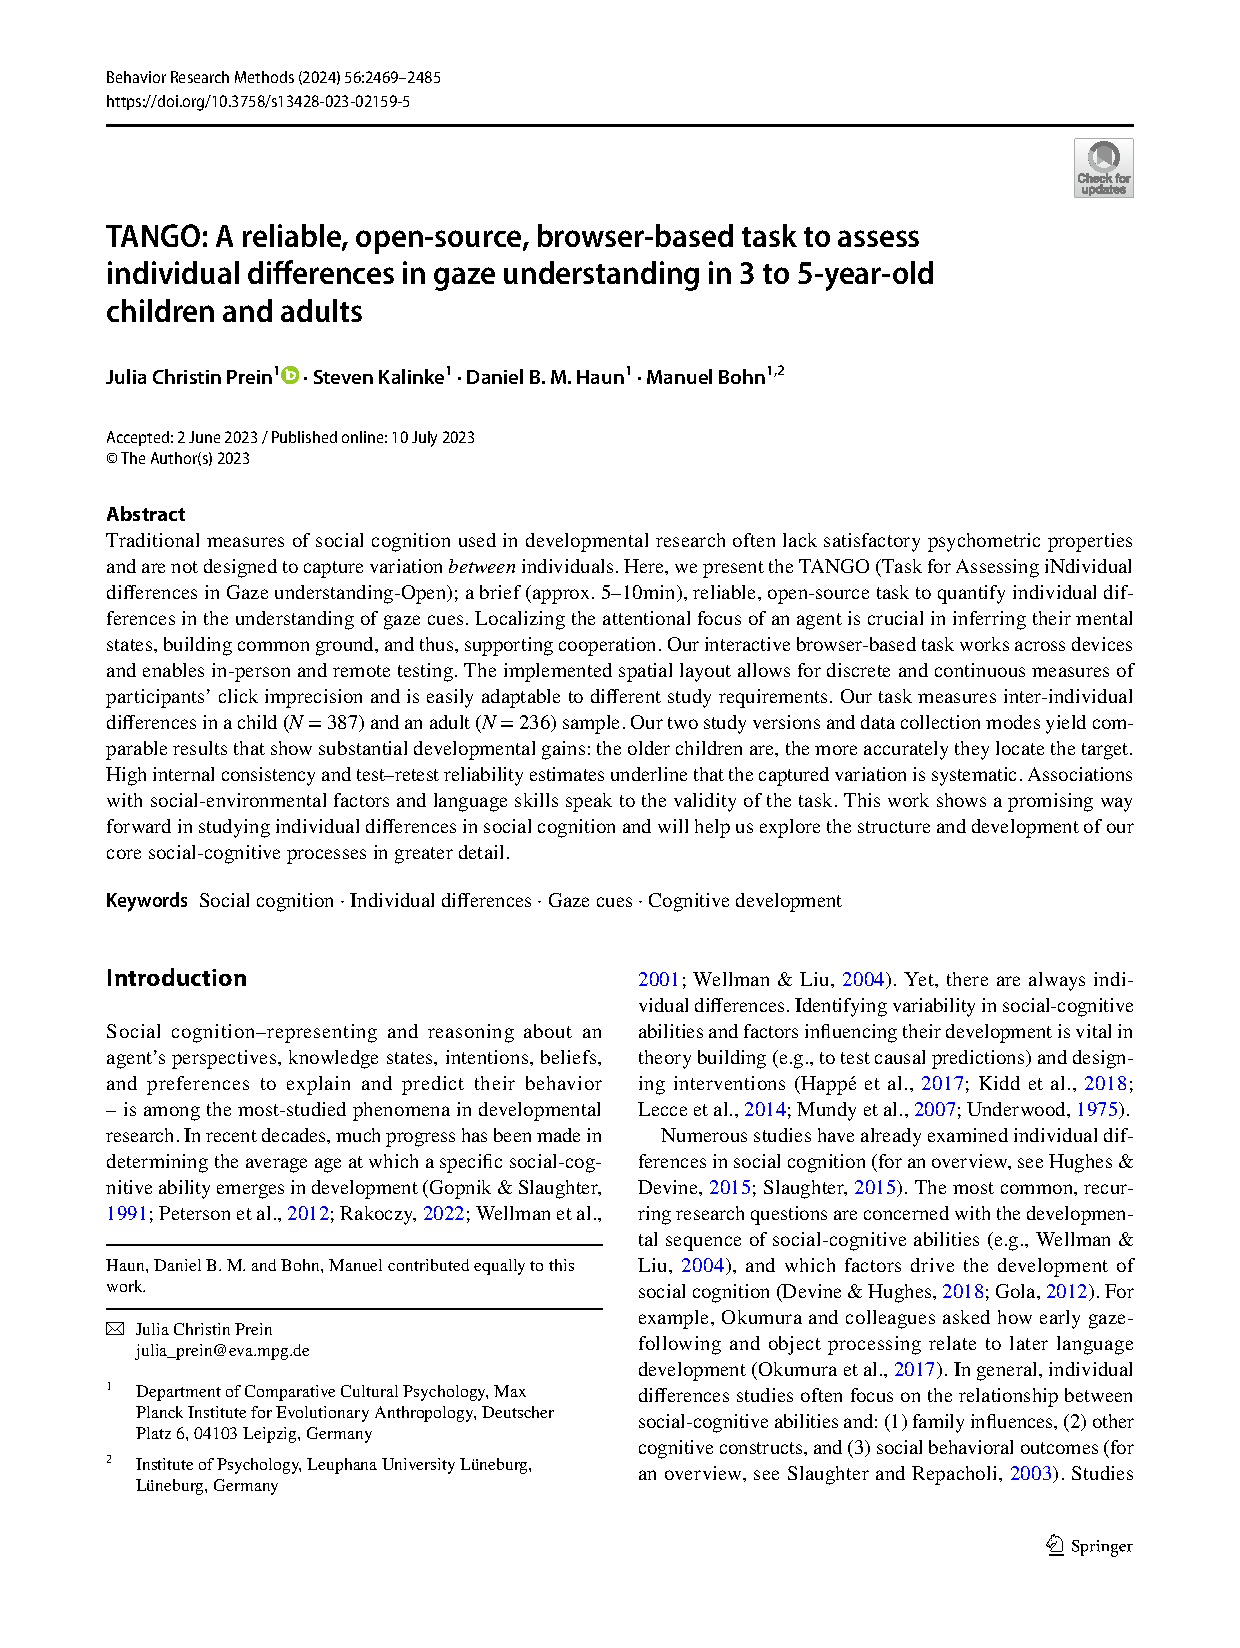
\includepdf[pages={1}, scale=0.85, offset=0 -1cm, pagecommand={}]{../papers/studyI.pdf}
\end{minipage}

\includepdf[pages={2-}, scale=0.85, pagecommand={}]{../papers/studyI.pdf}

\newpage

\section*{Study II}\label{studyII}
\addcontentsline{toc}{section}{Study II}

\begin{minipage}{\textwidth}
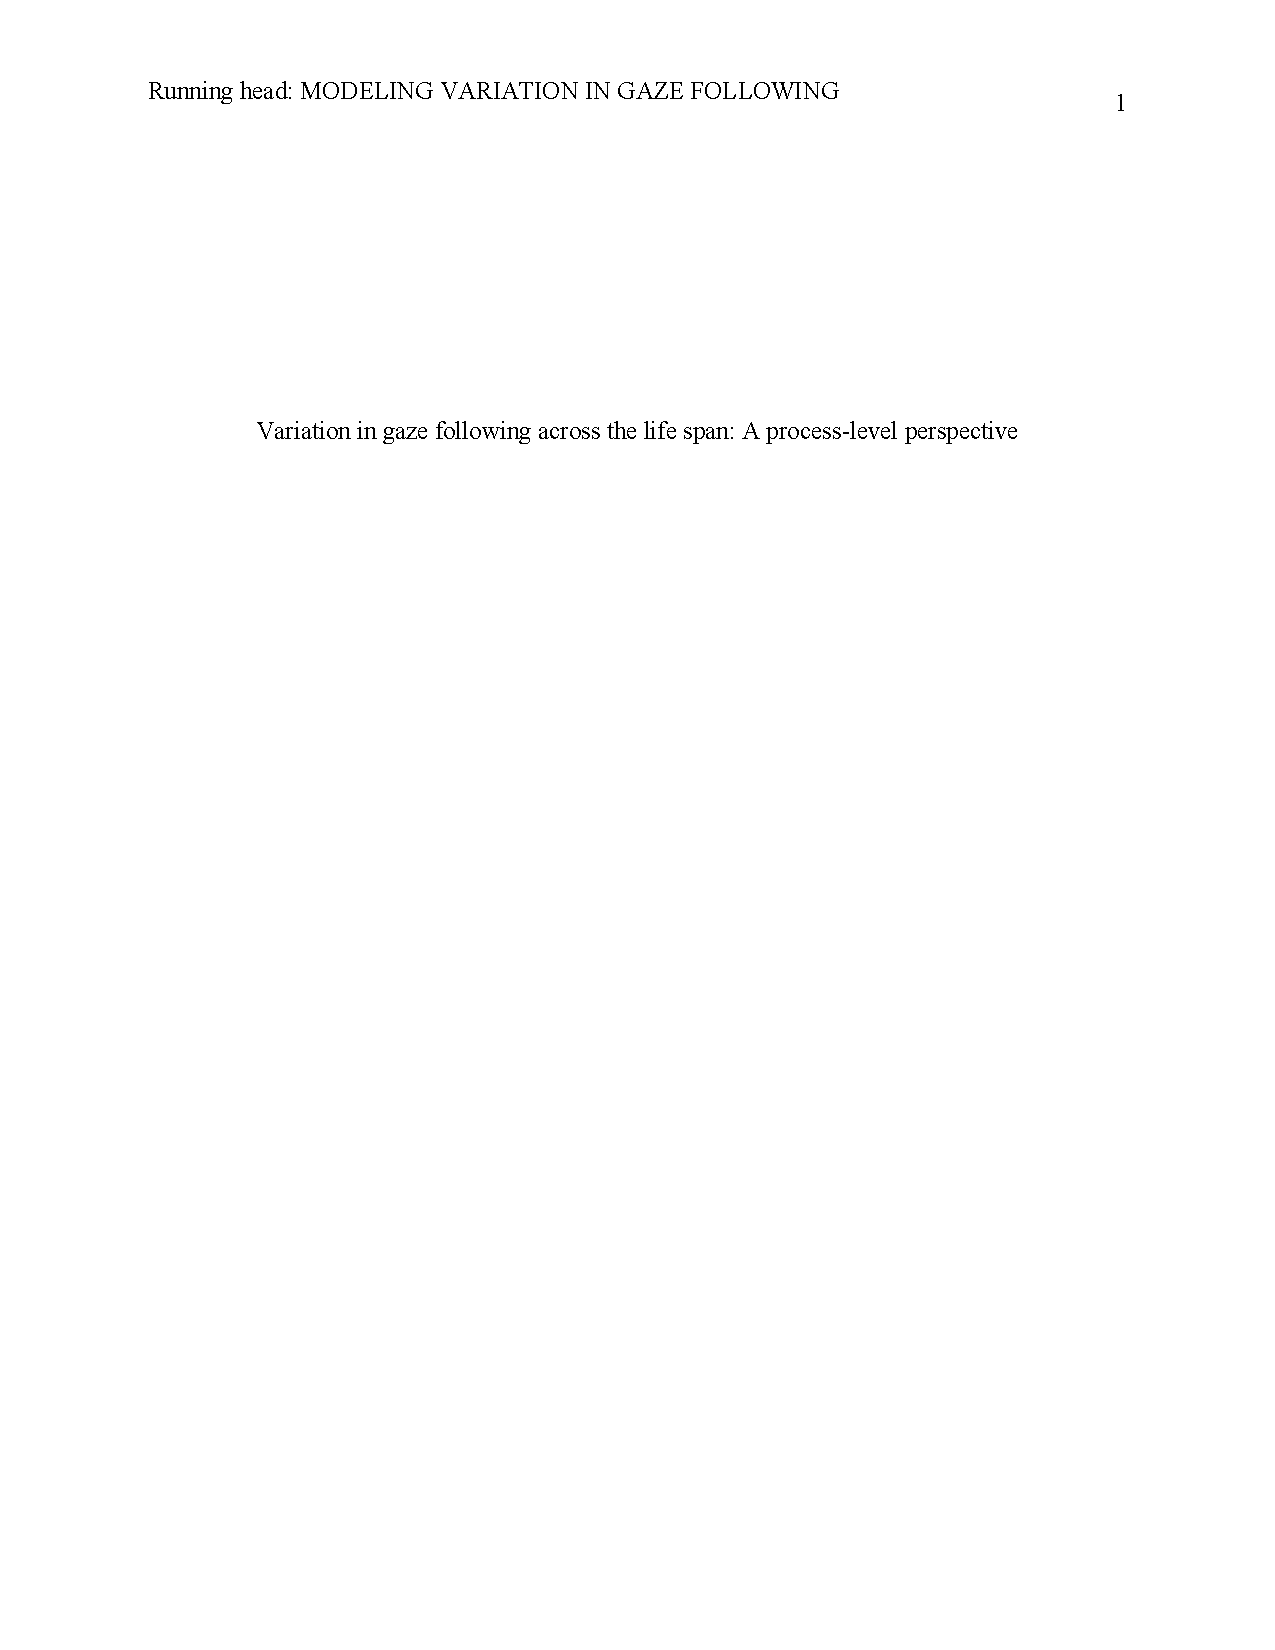
\includepdf[pages={1}, scale=0.85, offset=0 -1cm, pagecommand={}]{../papers/studyII.pdf}
\end{minipage}

\includepdf[pages={2-}, scale=0.85, pagecommand={}]{../papers/studyII.pdf}

\newpage

\section*{Study III}\label{studyIII}
\addcontentsline{toc}{section}{Study III}

\begin{minipage}{\textwidth}
\includepdf[pages={1}, scale=0.85, offset=0 -1cm, pagecommand={}]{../papers/studyIII.pdf}
\end{minipage}

\includepdf[pages={2-}, scale=0.85, pagecommand={}]{../papers/studyIII.pdf}

\newpage

\section*{Study IV}\label{studyIV}
\addcontentsline{toc}{section}{Study IV}

\begin{minipage}{\textwidth}
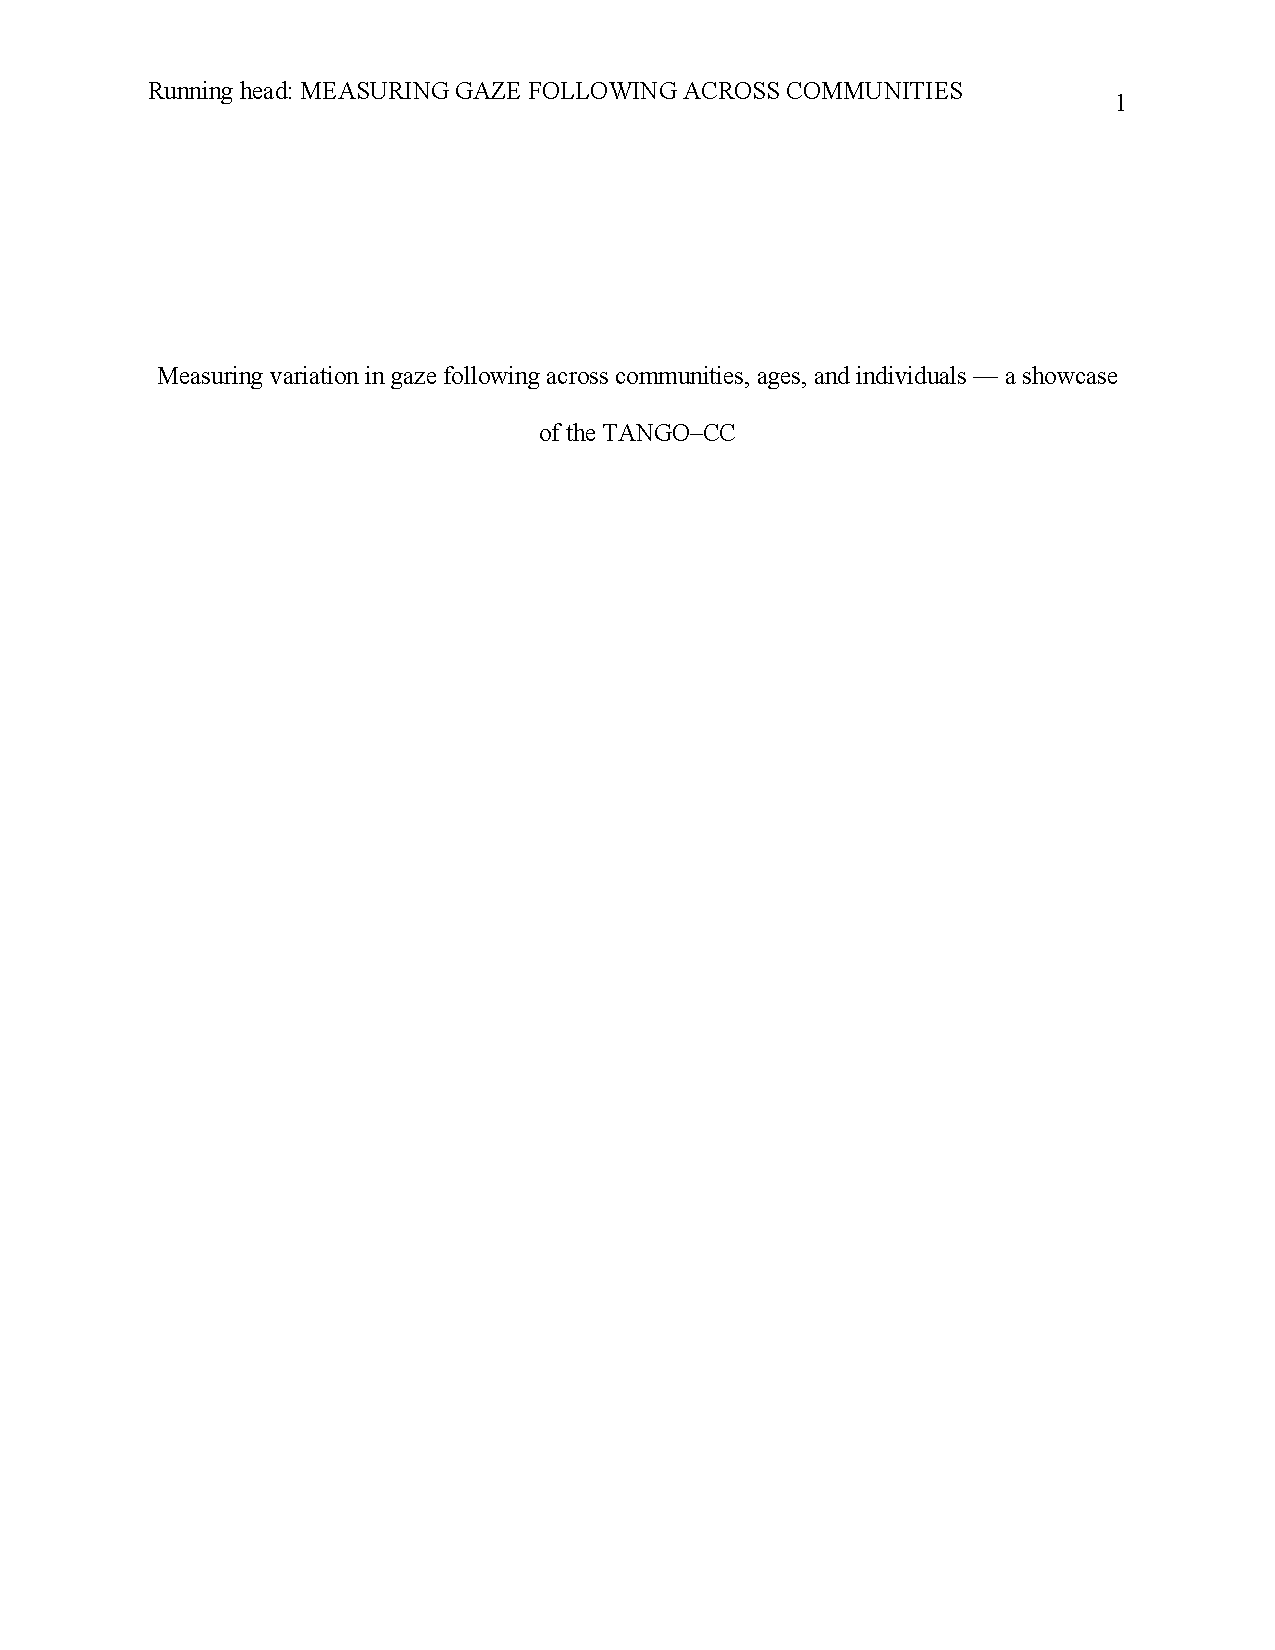
\includepdf[pages={1}, scale=0.85, offset=0 -1cm, pagecommand={}]{../papers/studyIV.pdf}
\end{minipage}

\includepdf[pages={2-}, scale=0.85, pagecommand={}]{../papers/studyIV.pdf}

\chapter*{Appendix B --- Further Publications}\label{appendixB}
\addcontentsline{toc}{chapter}{Appendix B --- Further Publications}

The following Appendix B contains other publications of side projects that were written in the context of the dissertation but not included in the main text, with their respective abstracts.

\section*{Action anticipation based on an agent's epistemic state in toddlers and adults}\label{manybabies}
\addcontentsline{toc}{section}{Action anticipation based on an agent's epistemic state in toddlers and adults}

\textbf{Citation:} Schuwerk, T., Kampis, D., Baillargeon, R., Biro, S., Bohn, M., Byers-Heinlein, K., Dörrenberg, S., Fisher, C., Franchin, L., Fulcher, T., Garbisch, I., Geraci, A., Grosse Wiesmann, C., Hamlin, K., Haun, D. B. M., Hepach, R., Hunnius, S., Hyde, D. C., Karman, P., \ldots, Prein, J., \ldots{} Rakoczy, H. (2021). \emph{Action anticipation based on an agent's epistemic state in toddlers and adults. Child Development} {[}In-Principle Acceptance of Registered Report Stage 1: Study Design{]}. PsyArXiv. \mbox{\url{https://doi.org/10.31234/osf.io/x4jbm}}

\textbf{Abstract:} Do toddlers and adults engage in spontaneous Theory of Mind (ToM)? Evidence from anticipatory looking (AL) studies suggests that they do. But a growing body of failed replication studies raised questions about the paradigm's suitability. In this multi-lab collaboration, we test the robustness of spontaneous ToM measures. We examine whether 18- to 27-month-olds' and adults' anticipatory looks distinguish between two basic forms of an agent's epistemic states: knowledge and ignorance. In toddlers {[}ANTICIPATED n = 520 50\% FEMALE{]} and adults {[}ANTICIPATED n = 408, 50\% FEMALE{]} from diverse ethnic backgrounds, we found {[}SUPPORT/NO SUPPORT{]} for epistemic state-based action anticipation. Future research can probe whether this conclusion extends to more complex kinds of epistemic states, such as true and false beliefs.

\emph{Please note that this abstract was written for the Registered Report and does not entail results yet. Text in square brackets indicates placeholder text to be filled in after data collection.}

\newpage

\section*{PREVIC: An adaptive parent report measure of expressive vocabulary in children between 3 and 8 years of age}\label{previc}
\addcontentsline{toc}{section}{PREVIC: An adaptive parent report measure of expressive vocabulary in children between 3 and 8 years of age}

\textbf{Citation:} Bohn, M., Prein, J. C., Engicht, J., Haun, D., Gagarina, N., \& Koch, T. (2023). \emph{PREVIC: An adaptive parent report measure of expressive vocabulary in children between 3 and 8 years of age.} {[}Manuscript submitted for publication{]}. PsyArXiv. \mbox{\url{https://doi.org/10.31234/osf.io/hvncp}}

\textbf{Abstract:} Parent report measures have proven to be a valuable research tool to study early language development. Caregivers are given a list of words and are asked which of them their child has already used. However, most available measures are not suited for children beyond infancy, come with substantial licensing costs or lack a clear psychometric foundation. Here we present the PREVIC (Parent Report of Expressive Vocabulary in Children), an open access, high quality vocabulary checklist for German-speaking children between three and eight years of age. The PREVIC was constructed leveraging the advantages of Item Response Theory: we designed a large initial item pool of 379 words and collected data from N = 1190 caregivers of children between three and eight years of age. Based on this data, we computed a range of fit indices for each item (word) and used an automated item selection algorithm to compile a final pool that contains items that a) vary in difficulty and b) fit the Rasch (one-parameter logistic) model. The resulting task is highly reliable and shows convergent validity. The IRT-based construction allowed us to design an adaptive version of the task, which substantially reduces the duration of the task while retaining measurement precision. The task -- including the adaptive version -- was implemented as a website and is freely accessible online (\mbox{\url{https://ccp-odc.eva.mpg.de/previc-demo/}}). The PREVIC fills an important gap in the toolkit of researchers interested in language development and provides an ideal starting point for the development of converging measures in other languages.

\newpage

\section*{oREV: An item response theory-based open receptive vocabulary task for 3- to 8-year-old children}\label{orev}
\addcontentsline{toc}{section}{oREV: An item response theory-based open receptive vocabulary task for 3- to 8-year-old children}

\textbf{Citation:} Bohn, M.*, Prein, J.*, Koch, T., Bee, R. M., Delikaya, B., Haun, D., \& Gagarina, N. (2024). oREV: An item response theory-based open receptive vocabulary task for 3- to 8-year-old children. \emph{Behavior Research Methods, 56}(3), 2595--2605. \mbox{\url{https://doi.org/10.3758/s13428-023-02169-3}}

\textbf{Abstract:} Individual differences in early language abilities are an important predictor of later life outcomes. High-quality, easy-access measures of language abilities are rare, especially in the preschool and primary school years. The present study describes the construction of a new receptive vocabulary task for children between 3 and 8 years of age. The task was implemented as a browser-based web application, allowing for both in-person and remote data collection via the internet. Based on data from N = 581 German-speaking children, we estimated the psychometric properties of each item in a larger initial item pool via item response modeling. We then applied an automated item selection procedure to select an optimal subset of items based on item difficulty and discrimination. The so-constructed task has 22 items and shows excellent psychometric properties with respect to reliability, stability, and convergent and discriminant validity. The construction, implementation, and item selection process described here makes it easy to extend the task or adapt it to different languages. All materials and code are freely accessible to interested researchers. The task can be used via the following website: \mbox{\url{https://ccp-odc.eva.mpg.de/orev-demo}}.

\newpage

\section*{Validation of an open source, remote web-based eye-tracking method (WebGazer) for research in early childhood}\label{manywebcams}
\addcontentsline{toc}{section}{Validation of an open source, remote web-based eye-tracking method (WebGazer) for research in early childhood}

\textbf{Citation:} Steffan, A., Zimmer, L., Arias-Trejo, N., Bohn, M., Dal Ben, R., Flores-Coronado, M. A., Franchin, L., Garbisch, I., Grosse Wiesmann, C., Hamlin, J. K., Havron, N., Hay, J. F., Hermansen, T. K., Jakobsen, K. V., Kalinke, S., Ko, E.-S., Kulke, L., Mayor, J., Meristo, M., \ldots, Prein, J., \ldots, Schuwerk, T. (2024). Validation of an open source, remote web-based eye-tracking method (WebGazer) for research in early childhood. \emph{Infancy, 29}(1), 31--55. \mbox{\url{https://doi.org/10.1111/infa.12564}}

\textbf{Abstract:} Measuring eye movements remotely via the participant's webcam promises to be an attractive methodological addition to in-person eye-tracking in the lab. However, there is a lack of systematic research comparing remote web-based eye-tracking with in-lab eye-tracking in young children. We report a multi-lab study that compared these two measures in an anticipatory looking task with toddlers using WebGazer.js and jsPsych. Results of our remotely tested sample of 18-27-month-old toddlers (N = 125) revealed that web-based eye-tracking successfully captured goal-based action predictions, although the proportion of the goal-directed anticipatory looking was lower compared to the in-lab sample (N = 70). As expected, attrition rate was substantially higher in the web-based (42\%) than the in-lab sample (10\%). Excluding trials based on visual inspection of the match of time-locked gaze coordinates and the participant's webcam video overlayed on the stimuli was an important preprocessing step to reduce noise in the data. We discuss the use of this remote web-based method in comparison with other current methodological innovations. Our study demonstrates that remote web-based eye-tracking can be a useful tool for testing toddlers, facilitating recruitment of larger and more diverse samples; a caveat to consider is the larger drop-out rate.

\chapter*{Appendix C --- Social Cognition Survey}\label{appendixC}
\addcontentsline{toc}{chapter}{Appendix C --- Social Cognition Survey}

In Autumn/Winter 2020, we conducted a short online expert survey on defining social cognition, as reported in the Introduction. Below you find the full survey, including the questions and the answers of the experts.

\begin{minipage}{\textwidth}
\includepdf[pages={1}, scale=0.85, offset=0 -1cm, pagecommand={}]{../supplements/social_cognition_survey.pdf}
\end{minipage}

\includepdf[pages={2-}, scale=0.85, pagecommand={}]{../supplements/social_cognition_survey.pdf}

\newpage

\chapter{Acknowledgments}\label{acknowledgments}

This dissertation rests on the shoulders of many inspiring, thought-provoking, motivating, and caring individuals. The last four years have been many different things\thinspace --\thinspace but definitely neither boring nor stagnant. I want to thank everyone who has accompanied me on this journey.

My motivation to work on this dissertation is greatly due to my wonderful supervisors. Manuel, I cannot thank you enough for supporting me. You have taught me to critically challenge the status quo in research and to focus my energy on improving it\thinspace --\thinspace pragmatically, step by step. Even though I do know that you believe there \emph{are} stupid questions, I felt very comfortable to ask you all along the way and I have benefited a lot from your patience with me. Thanks for roughly 200 meetings that have always left me more motivated and focused than I was before. Daniel, I am so happy and proud to have been a member of the CCP team. Thank you for offering me so many unique opportunities and unforgettable memories, like traveling to conferences and Uganda. I am deeply impressed by how quickly you get a grasp of a new project and know immediately which questions to ask. Thank you for being such an approachable director and having an open door to hear about my personal struggles and have philosophical discussions. To my external supervisor, Robert: your teaching in Research Methods has turned my hate for statistics into a deep passion. Thanks for encouraging me to do a PhD, for looking into open positions, and accompanying me along the way.

Thanks to all the people who made my travels to Uganda so enjoyable. I want to express my gratitude to the members of the Budongo Families Project, especially Florence, Agnes, Joan and Joseph\thinspace --\thinspace for your warm welcome, all your help, hard work and heartfelt laughter.

Thanks to the people at Leuphana who made my arrival in Lüneburg so much easier. Sebastian, thank you for making it possible for me to pursue this doctoral title. Patricia, Franziska, Nele, and (again) Manuel, thanks for the welcoming and kind atmosphere in the LüneLütten lab. I am excited about what is to come next!

I am grateful to our wonderful cohort of PhDs at the MPI. You are a remarkable group of people, and I am very happy that we could share our daily struggles with each other. Noemi, I am so glad that we got to share our office for a (way too short) period of time and successfully solved the Christmas murder mystery with Marie. Wilson, thanks for enduring our laughter through the office walls, for countless lunch breaks together, and for sharing random stories about your fieldwork (and Iceland)! Without my work wife Marie, my time during this dissertation would not have been even half as great as it has been. You have made me laugh so much, even if all I wanted to do was cry. Whatever it is that I am up to, I know you will always have my back and help me get back on my feet if I fail. I love your honesty, creativity, immense courage, charming awkwardness, and quirky sense of humor, and feel so honored that you are my friend. Thank you for being you!

My dear, dear family, I am so deeply grateful to know you by my side. Whenever I talk about individual differences, I think about you, Caro, and how we two sisters have the same parents and yet, are so different (in the very best way!!). I believe it is rare that siblings do not feel the need to compete with each other but can just love each other as they are. Thank you! To my mom, who told me right in the beginning that this journey would be a marathon and not a sprint. In some of my darker moments, you told me that even if it felt like I was about to fall, I could never\thinspace --\thinspace because there are so many caring people who would catch me beforehand. Thank you for always having an open home and lots of support (in the form of love, food, vacations, phone calls, and advice) for me. To my dad, thanks for showing up to Leipzig so often and establishing a little concert routine together! I believe I have learned a lot of my problem-solving skills and patience from you. Even if you do not remember saying ``Mach Dinge richtig'' in Caro's and my childhood, I think my dissertation has greatly benefited from this sentence. Thank you, Louis, for helping with my move to Leipzig and spontaneously catching up over coffee in Leipzig or Berlin. To my grandpa, who told me he never worried that I would find my own way. And to my grandma, for all your curiosity, play, and love for children. To the whole Gerken-Prein clan (including our furry friends)\thinspace --\thinspace I could not wish for a better family. Finally, we are reunited in the North.

Thank you to my amazing friends, who constantly remind me to live my life outside the office. To O74, OLAV, and Shubhangi, Schlotti, and Maló, for the cozy home we built together. All our little dance breaks, kitchen karaoke, and reading clubs made even COVID isolation fun. Thanks for your patience with my mood swings and stealing lunch boxes! Thanks to Laura, for drying my tears, always having an open ear and heart, and helping me with every single move. To Marvin, for all the long hours of deep talk and starting the whole dancing journey with me. To the Kizomba community, especially Carlos and Benedikta, for forcing me to close my eyes, shut off my brain, and relax. Thanks to Arne, for nerding about statistics and providing way too much Pfeffi. To the Osna Coxis, especially Merle, Leah, and Alissa, for all the New Year's Eves, regular video calls, big hugs and words of comfort. To Niki, for constantly reaching out, joking around, and asking me how I'm doing. To Ani, Nica, and Schlotti for a lifelong friendship, wholehearted laughter, and a traveling diary. I am so grateful to have every single one of you in my life.

And finally, Steven. You have taken over so many different roles in my life over the last four years. In the beginning, I was simply grateful for your technological support and coding enthusiasm. Thank you for pushing me beyond my levels of comfort and believing in my programming skills (\ldots{} and for being my IT partner ;)). But then, coding became only one of the thousand topics that we would regularly discuss. Every morning, I looked forward to you making creepy, funny faces on our office door and having long, controversial, and nerdy conversations with you. I deeply miss you in my daily work life. And yet, I do appreciate all the changes that our relationship has gone through\thinspace --\thinspace through all the highs and lows. I am sincerely grateful and glad to share my life with you. It is so easy being myself around you. Thank you for the commitment, stability, honesty, relaxation, music, joy, and silly jokes that you bring into my life. Your love and support means the world to me. I cannot wait for our new adventures together in Hamburg!

\chapter*{Selbstständigkeitserklärung}\label{selbststaendigkeit}
\addcontentsline{toc}{chapter}{Selbstständigkeitserklärung}

Julia Christin Prein\\
{[}Straße Hausnummer{]}\\
{[}PLZ Ort{]}\\
{[}Telefon{]}\\
{[}Email{]}\\

Hiermit erkläre ich, dass ich mich noch keiner Doktorprüfung unterzogen oder mich um Zulassung zu einer solchen beworben habe.

Ich versichere, dass die Dissertation \emph{Rethinking Variation in Social Cognition: Gaze Following across Individuals, Ages, and Communities} in der gegenwärtigen oder einer anderen Fassung noch keiner anderen Hochschule zur Begutachtung vorgelegen hat.

Ich versichere an Eides statt, dass ich die eingereichte Dissertation \emph{Rethinking Variation in Social Cognition: Gaze Following across Individuals, Ages, and Communities} selbstständig und ohne zulässige fremde Hilfe verfasst habe. Anderer als der von mir angegebenen Hilfsmittel und Schriften habe ich mich nicht bedient. Alle wörtlich oder sinngemäß anderen Schriften entnommenen Stellen habe ich kenntlich gemacht. Über die strafrechtlichen Folgen gemäß § 156 Strafgesetzbuch wurde ich in Kenntnis gesetzt.

~

Hamburg, {[}Datum{]}

~

{[}Unterschrift{]}

\end{document}
